\documentclass{beamer}

\usepackage{beamerthemesplit}
\usepackage{verbatim}
\usepackage[normalem]{ulem}

\usepackage{xcolor}

\usepackage{hyperref}

\definecolor{gold}{rgb}{1.,0.84,0.}
\definecolor{brightred}{rgb}{1.,0.4,0.4}
\definecolor{mygray}{RGB}{200,200,200}
\definecolor{lightsteelblue}{RGB}{176,196,222}
\definecolor{lightskyblue}{RGB}{135,206,250}
\definecolor{cadetblue}{RGB}{95,158,160}

\usetheme{default}
\usecolortheme{mule}

\usefonttheme{serif}

%\DeclareGraphicsExtensions{.pdf,.png,.jpg}

\newcommand{\mcal}{\textsc{metacalibration}}
\newcommand{\Mcal}{\textsc{Metacalibration}}


\title{Using Gravitational Lensing to measure Dark Matter and Dark Energy in
the Universe}
\author{Erin Sheldon}
\institute{Brookhaven National Laboratory}

% http://texblog.net/latex-archive/plaintex/beamer-footline-frame-number/
% to add the page (frame ) number and not screw up the bottom line
% works for split themes?
\expandafter\def\expandafter\insertshorttitle\expandafter{%
      \insertshorttitle\hfill%
        \insertframenumber\,/\,\inserttotalframenumber}

% suppress navigation bar
\beamertemplatenavigationsymbolsempty
\setbeamertemplate{footline}{}

\begin{document}

\usebackgroundtemplate{%
    %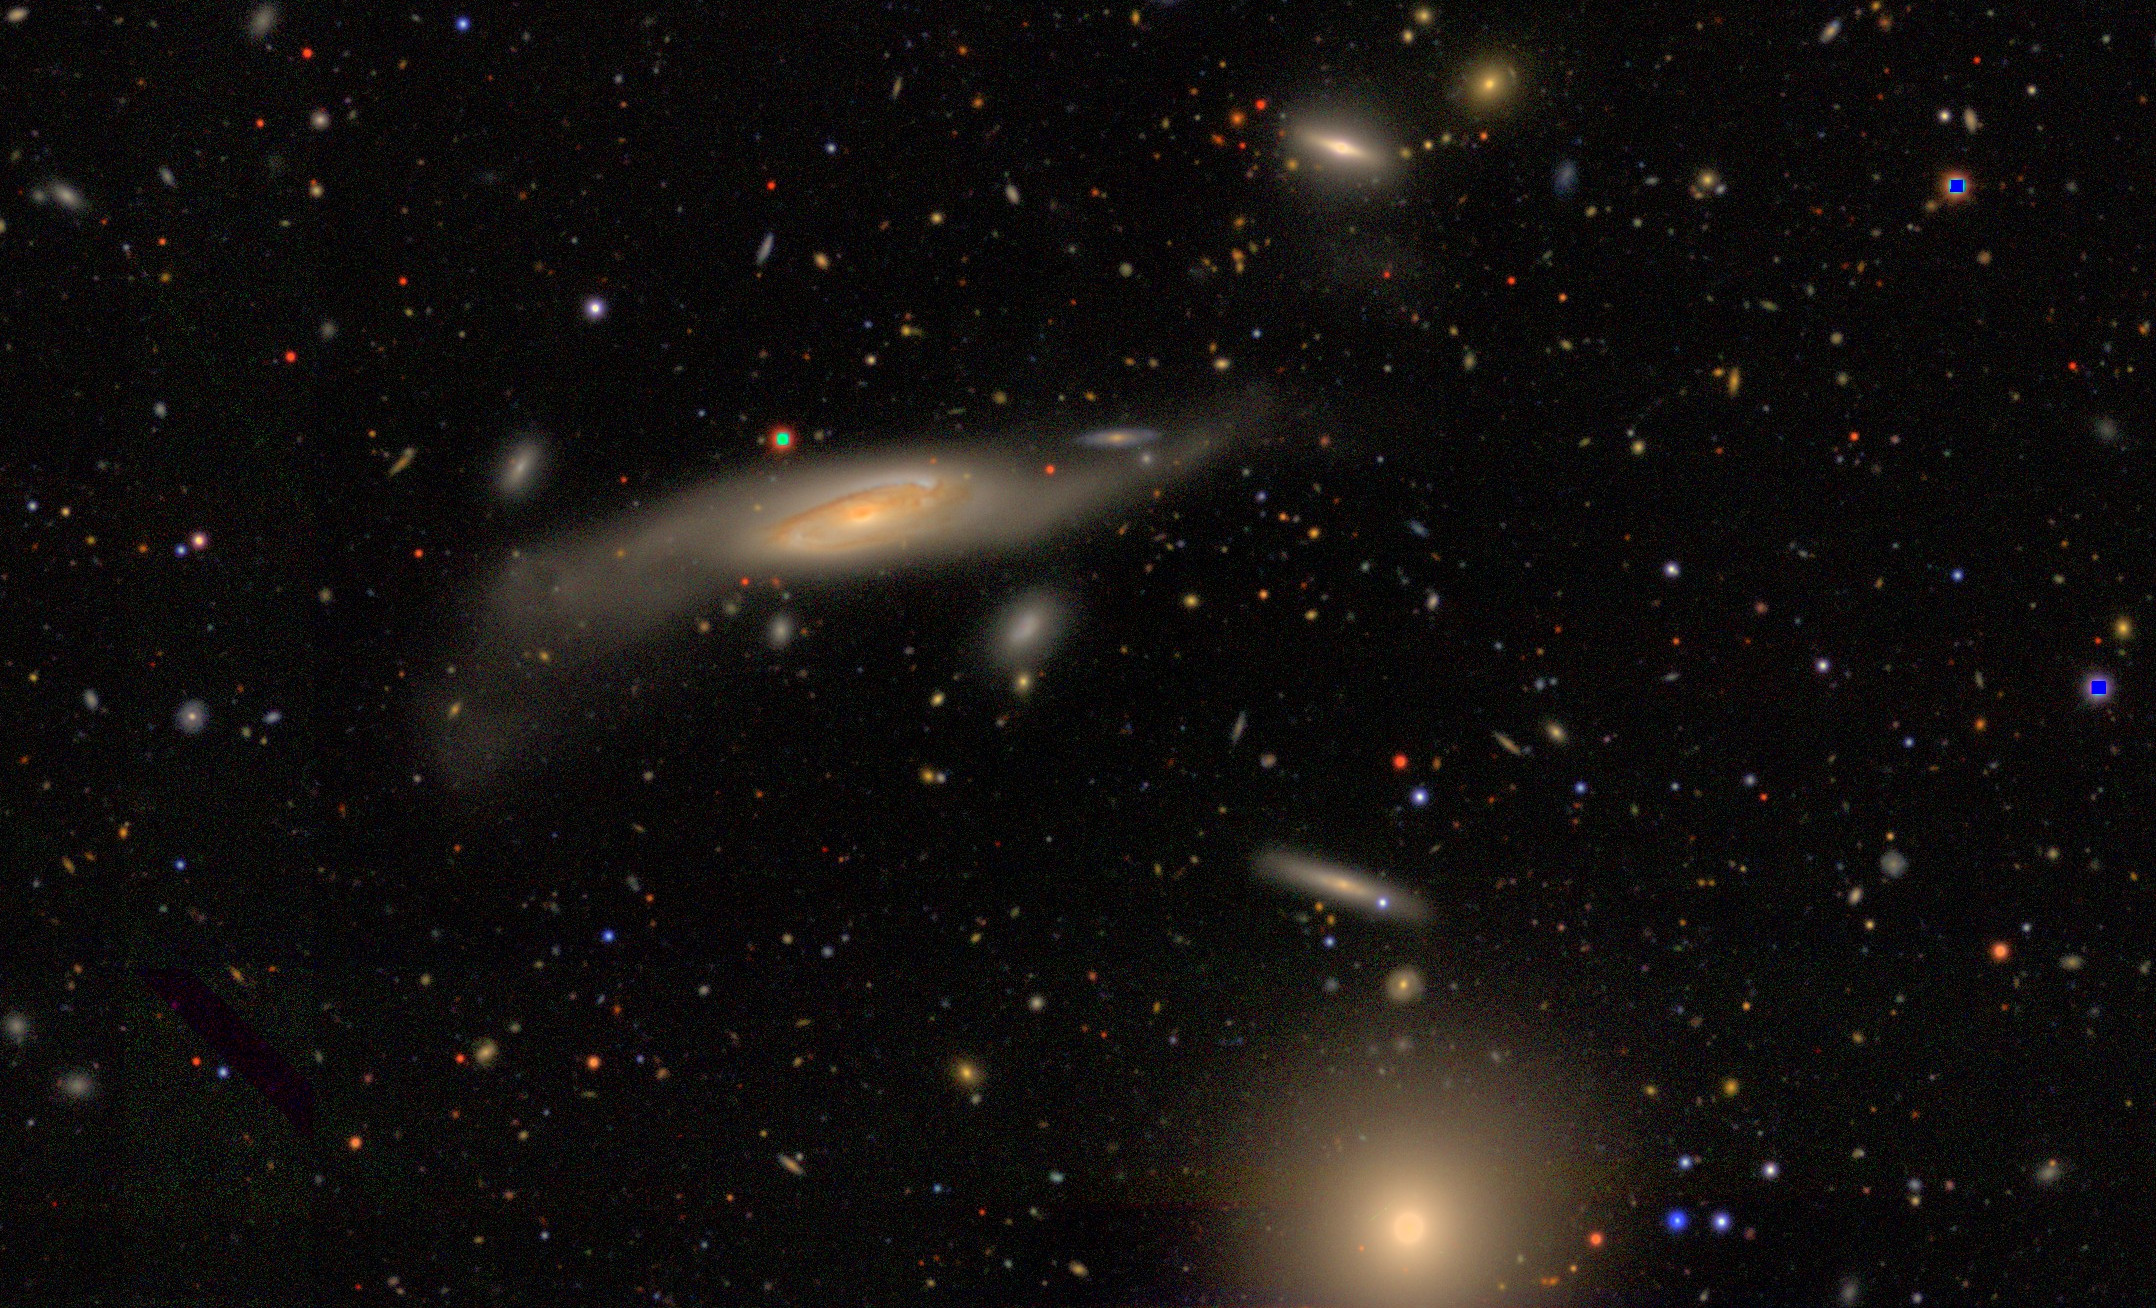
\includegraphics[height=\paperheight]{DES0056-5248_gri_crop.jpg}}
\includegraphics[trim=100 0 0 0,clip,height=\paperheight]{DES-2013-01-medres.jpg}}
\frame
{
}
\setbeamertemplate{background canvas}[vertical shading][bottom=mgray,top=mblack]



\frame{\titlepage}


\setbeamerfont*{itemize/enumerate body}{size=\Large}
\setbeamerfont*{itemize/enumerate subbody}{parent=itemize/enumerate body}
\setbeamerfont*{itemize/enumerate subsubbody}{parent=itemize/enumerate body}

\frame
{
    \frametitle{About This Lecture}

    \setbeamerfont*{itemize/enumerate body}{size=\large}

    \begin{itemize}

        \item The target audience is students who have taken an intro-level
            physics class at university.
            
        \item I'm also relying on some information the intro to cosmology by
            Paul Stankus.

        \item My goal is to introduce basic concepts and give some examples

        \item Feel free to ask questions, {\em I don't care if I get through 
            all of the material}

        \item In the interest of pedagogy, I ask those in the room with PhDs to
            please refrain from commenting or asking questions :)

    \end{itemize}

}



\frame
{
    \frametitle{Outline}


    \begin{itemize}

        \item Very brief introduction to cosmology
        \item Introduction to Gravitational Lensing
        \item How we learn about cosmology using lensing
        \item Some examples

    \end{itemize}

}

\frame
{

    {\huge Cosmology}

}

\frame
{
    \frametitle{Introduction to Cosmology}


    \begin{itemize}

        \item I'm building off of Paul's lecture on cosmology.

        \item I'll focus on the main topics pertaining to lensing

        %\item What makes up the universe? What can we see?

        %\item Where is it all?  How is matter distributed?

        %\item What is the history of the universe?

        %\item Can we explain what we see?  Is what we see consistent with our
        %    understanding of fundamental physics?

    \end{itemize}

}


\frame
{

    \frametitle{What Makes Up the Universe?}

    \setbeamerfont*{itemize/enumerate body}{size=\large}

    \begin{columns}
        \begin{column}{0.5\textwidth}
            \begin{itemize}


                \item Particles -- people -- planets -- stars -- galaxies

                \item What is the composition of distant objects?

                \item What is the mass density of the universe?

                \item What fraction of the mass in the universe
                    is dark matter?

            \end{itemize}
        \end{column}
        \begin{column}{0.5\textwidth}
            \begin{center}
                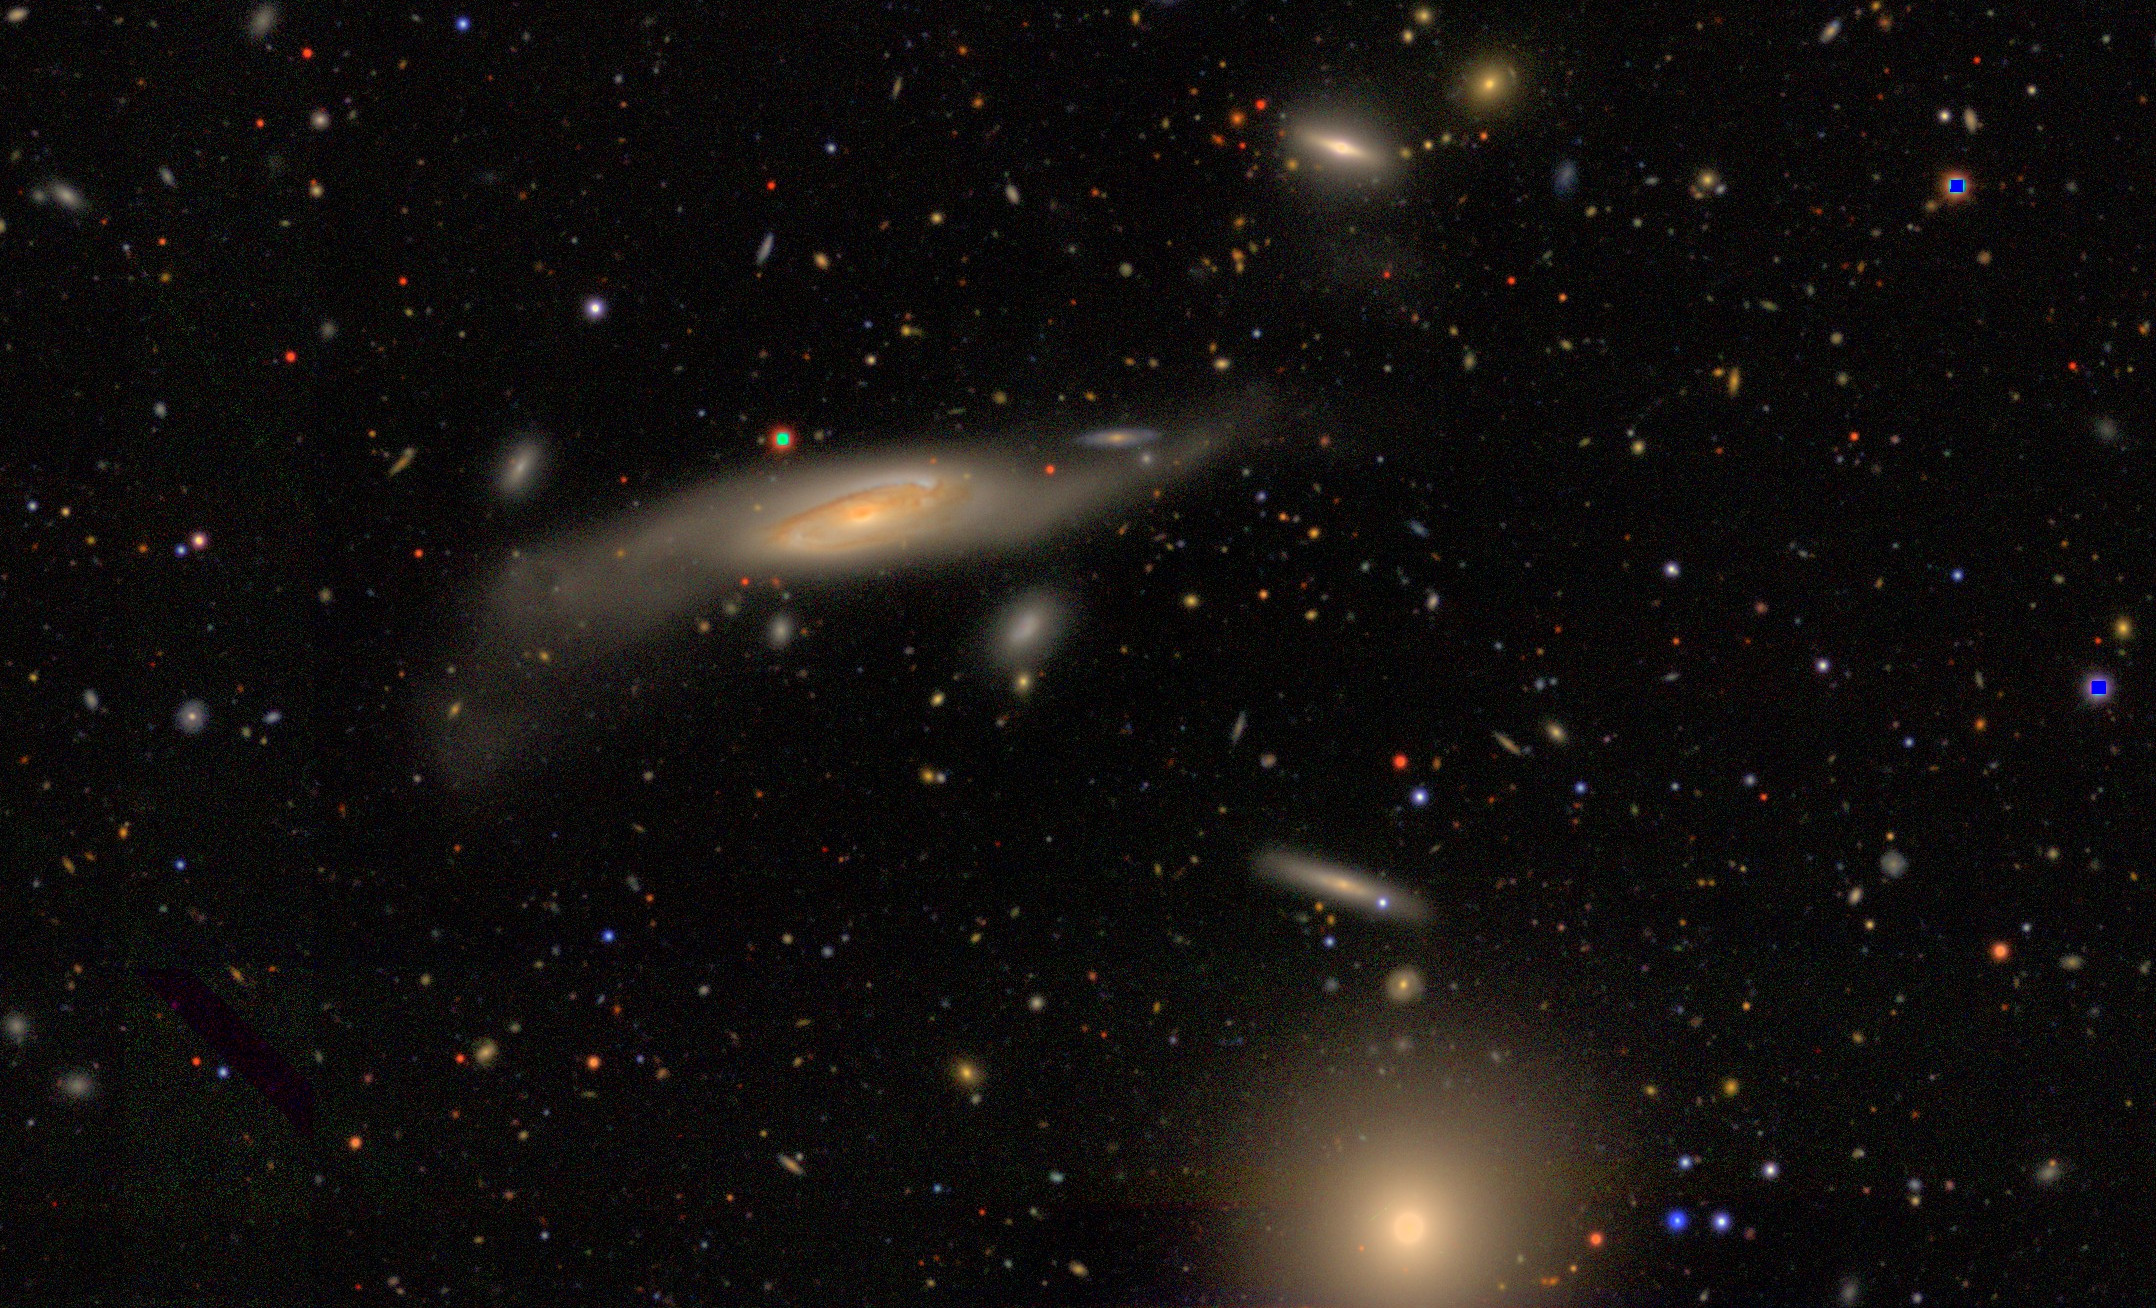
\includegraphics[width=1.2\textwidth, angle=90]{DES0056-5248_gri_crop.jpg}
                \newline
                {\tiny DES/Erin Sheldon}
            \end{center}
        \end{column}
    \end{columns}


}

\usebackgroundtemplate{%
    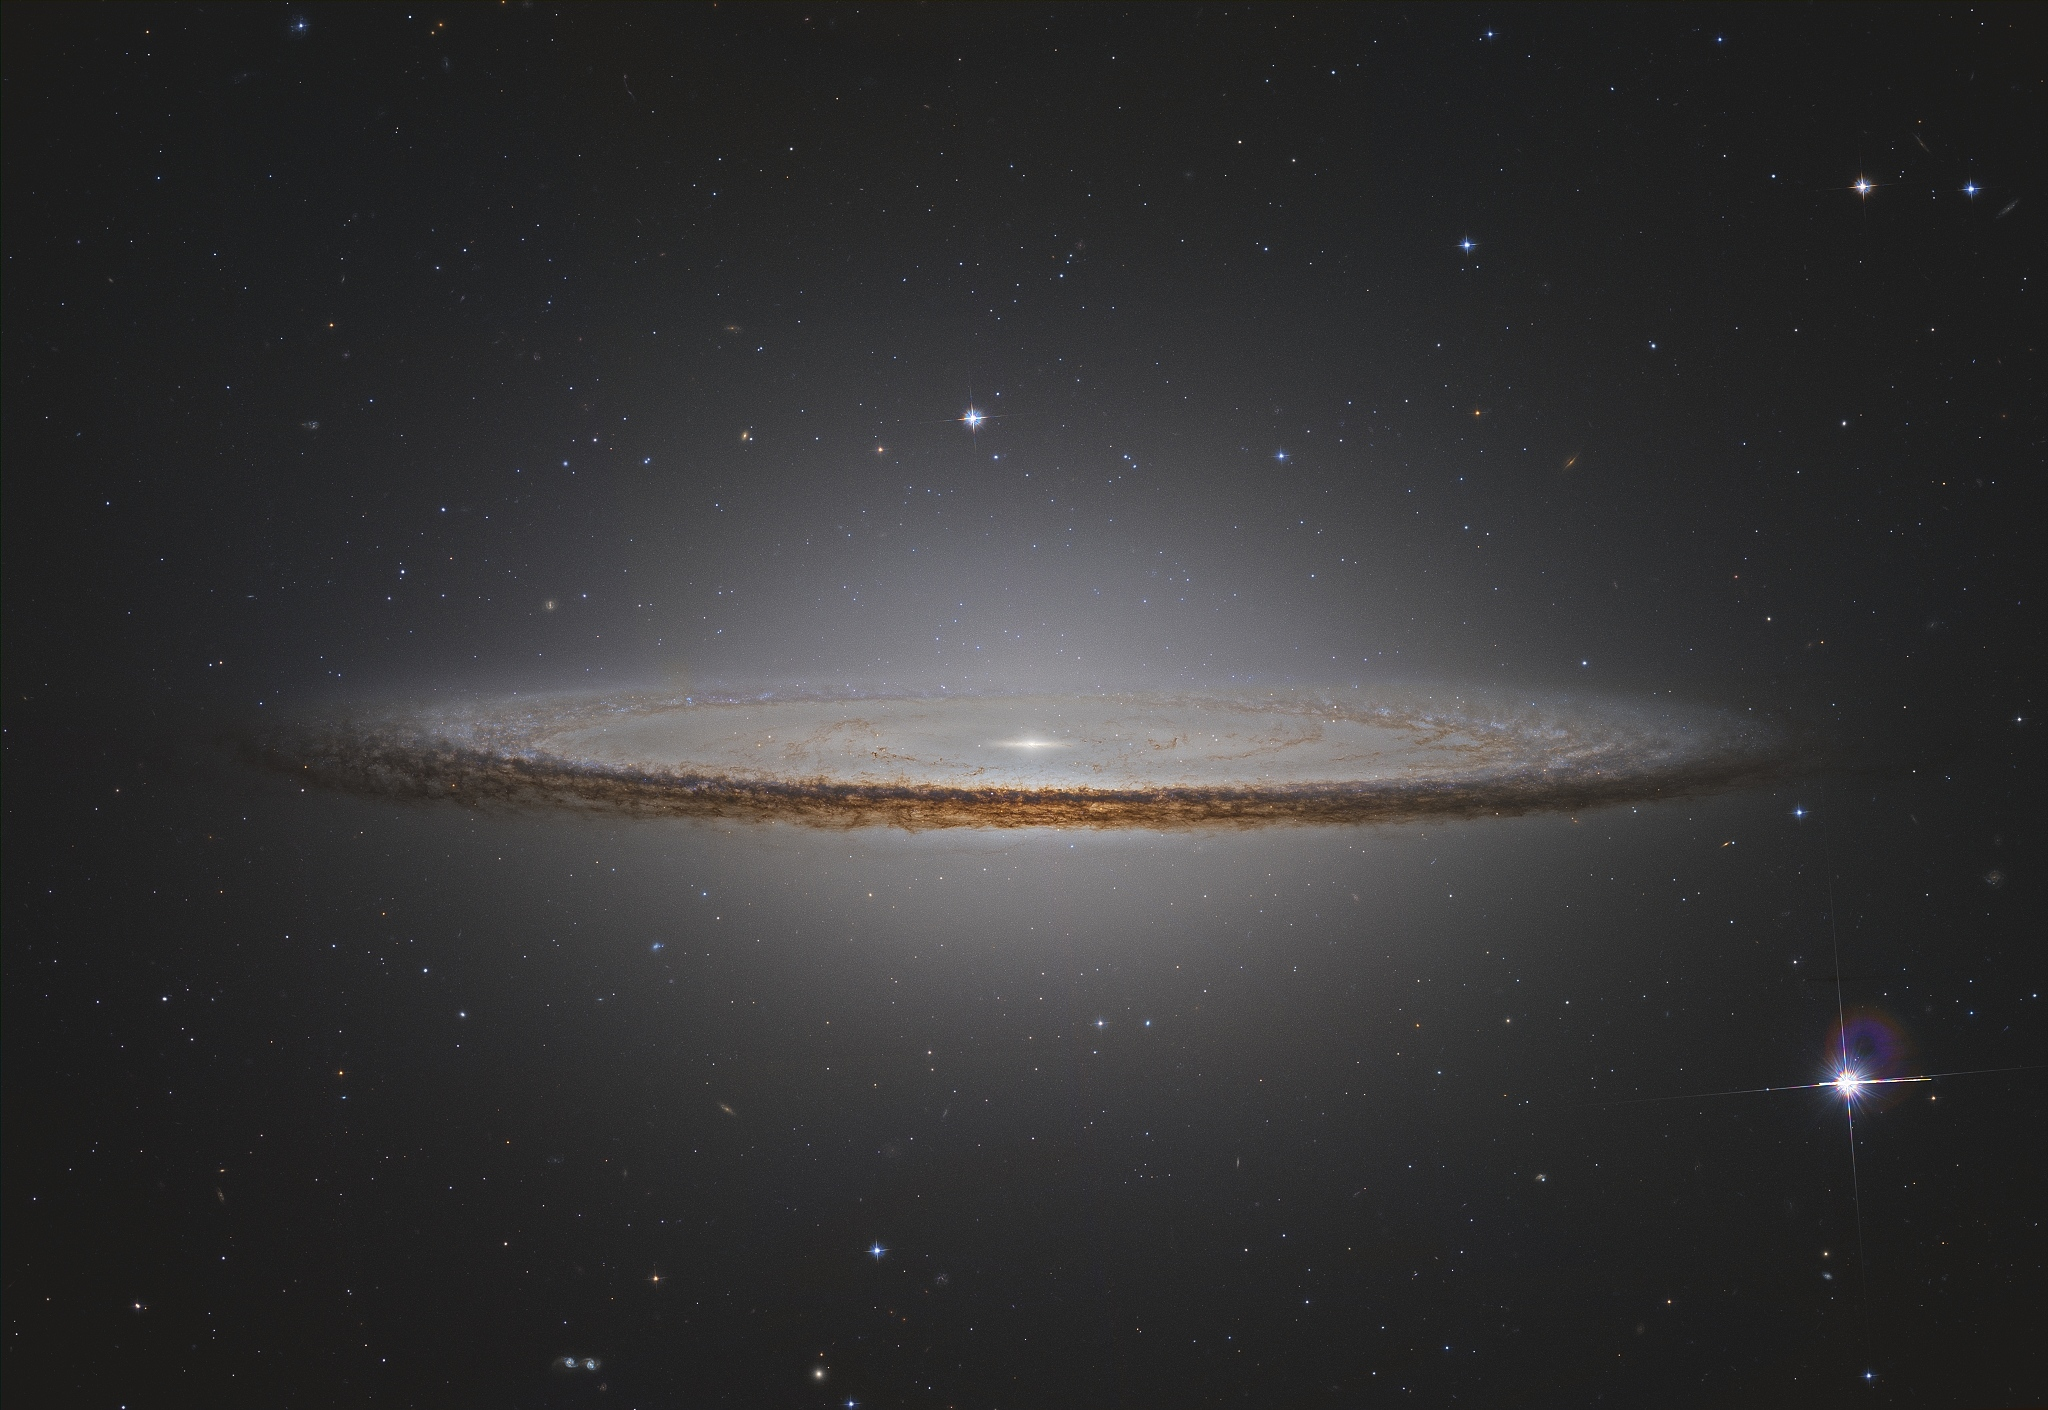
\includegraphics[width=\paperwidth,height=\paperheight]{M104b_peris2048.jpg}
}
\frame
{
}
\setbeamertemplate{background canvas}[vertical shading][bottom=mgray,top=mblack]


\frame
{

    \frametitle{How is matter distributed?}

    \setbeamerfont*{itemize/enumerate body}{size=\large}

    \begin{columns}
        \begin{column}{0.5\textwidth}
            \begin{itemize}

                \item Where are the galaxies and dark matter in the universe,
                    over large scales?

            \end{itemize}
        \end{column}
        \begin{column}{0.5\textwidth}
            \begin{center}
                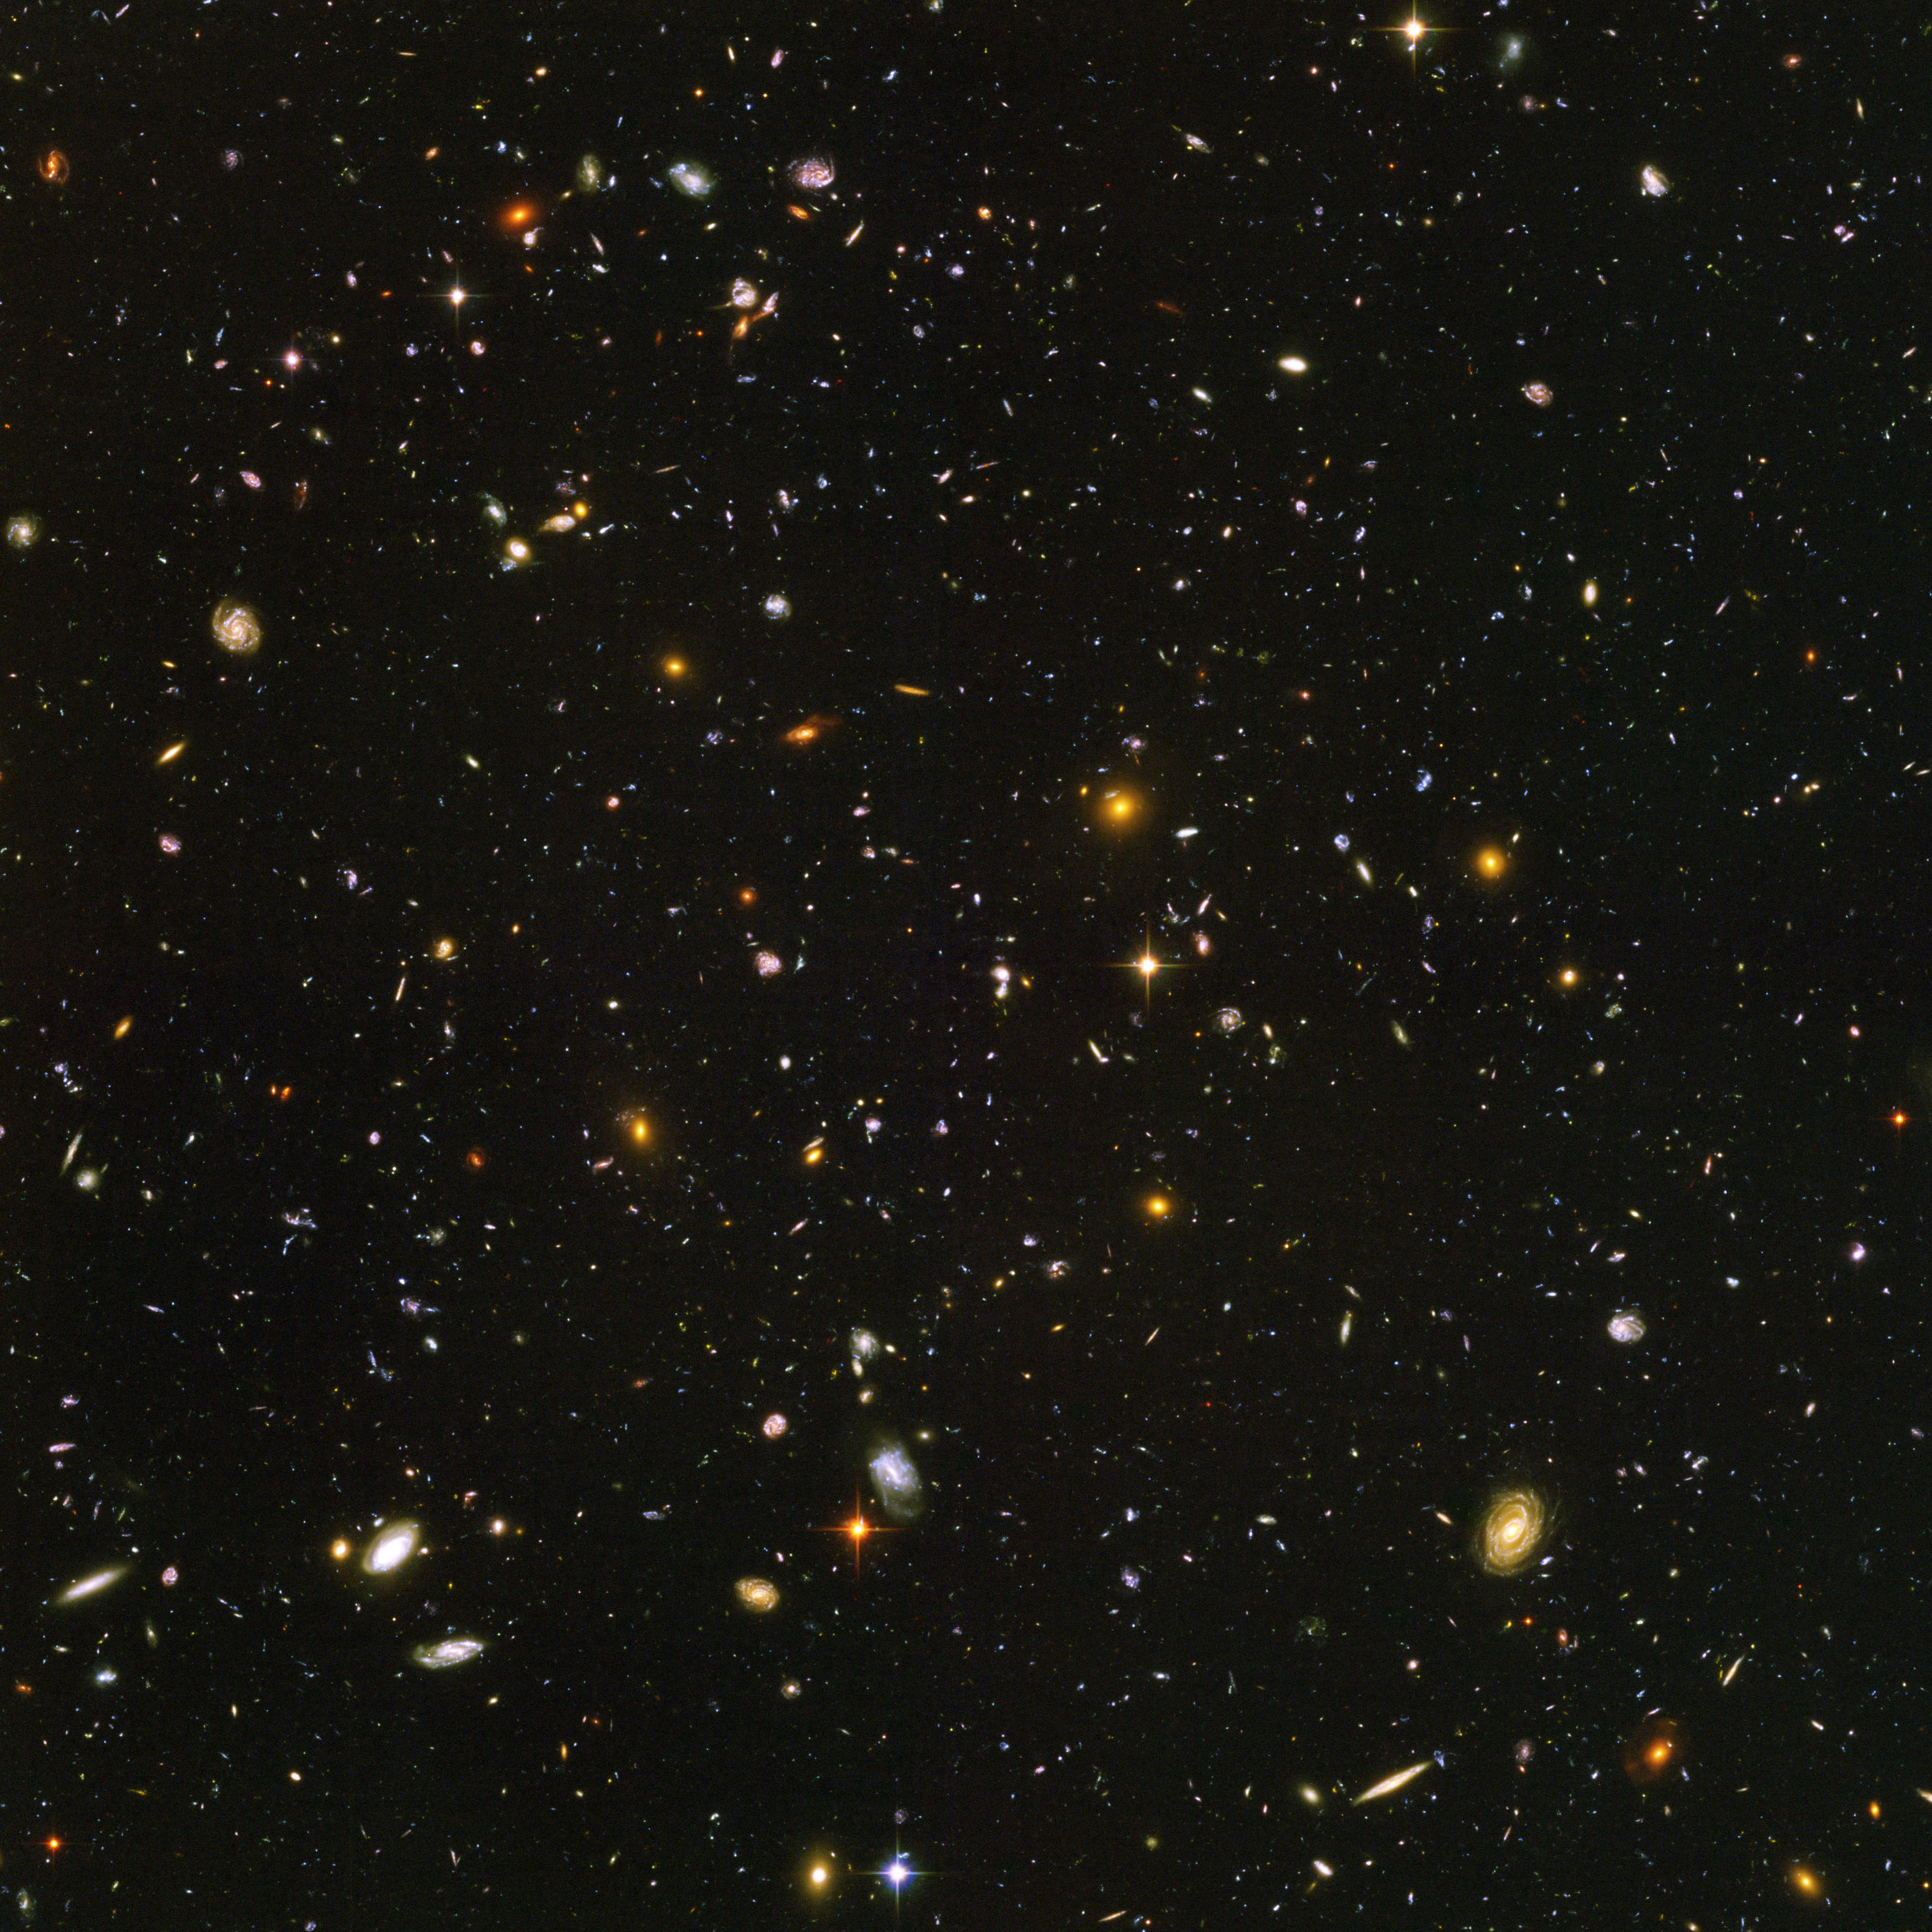
\includegraphics[width=\textwidth]{UDF_half.jpg}
            \end{center}
        \end{column}
    \end{columns}


}


\frame
{
    \begin{center}
        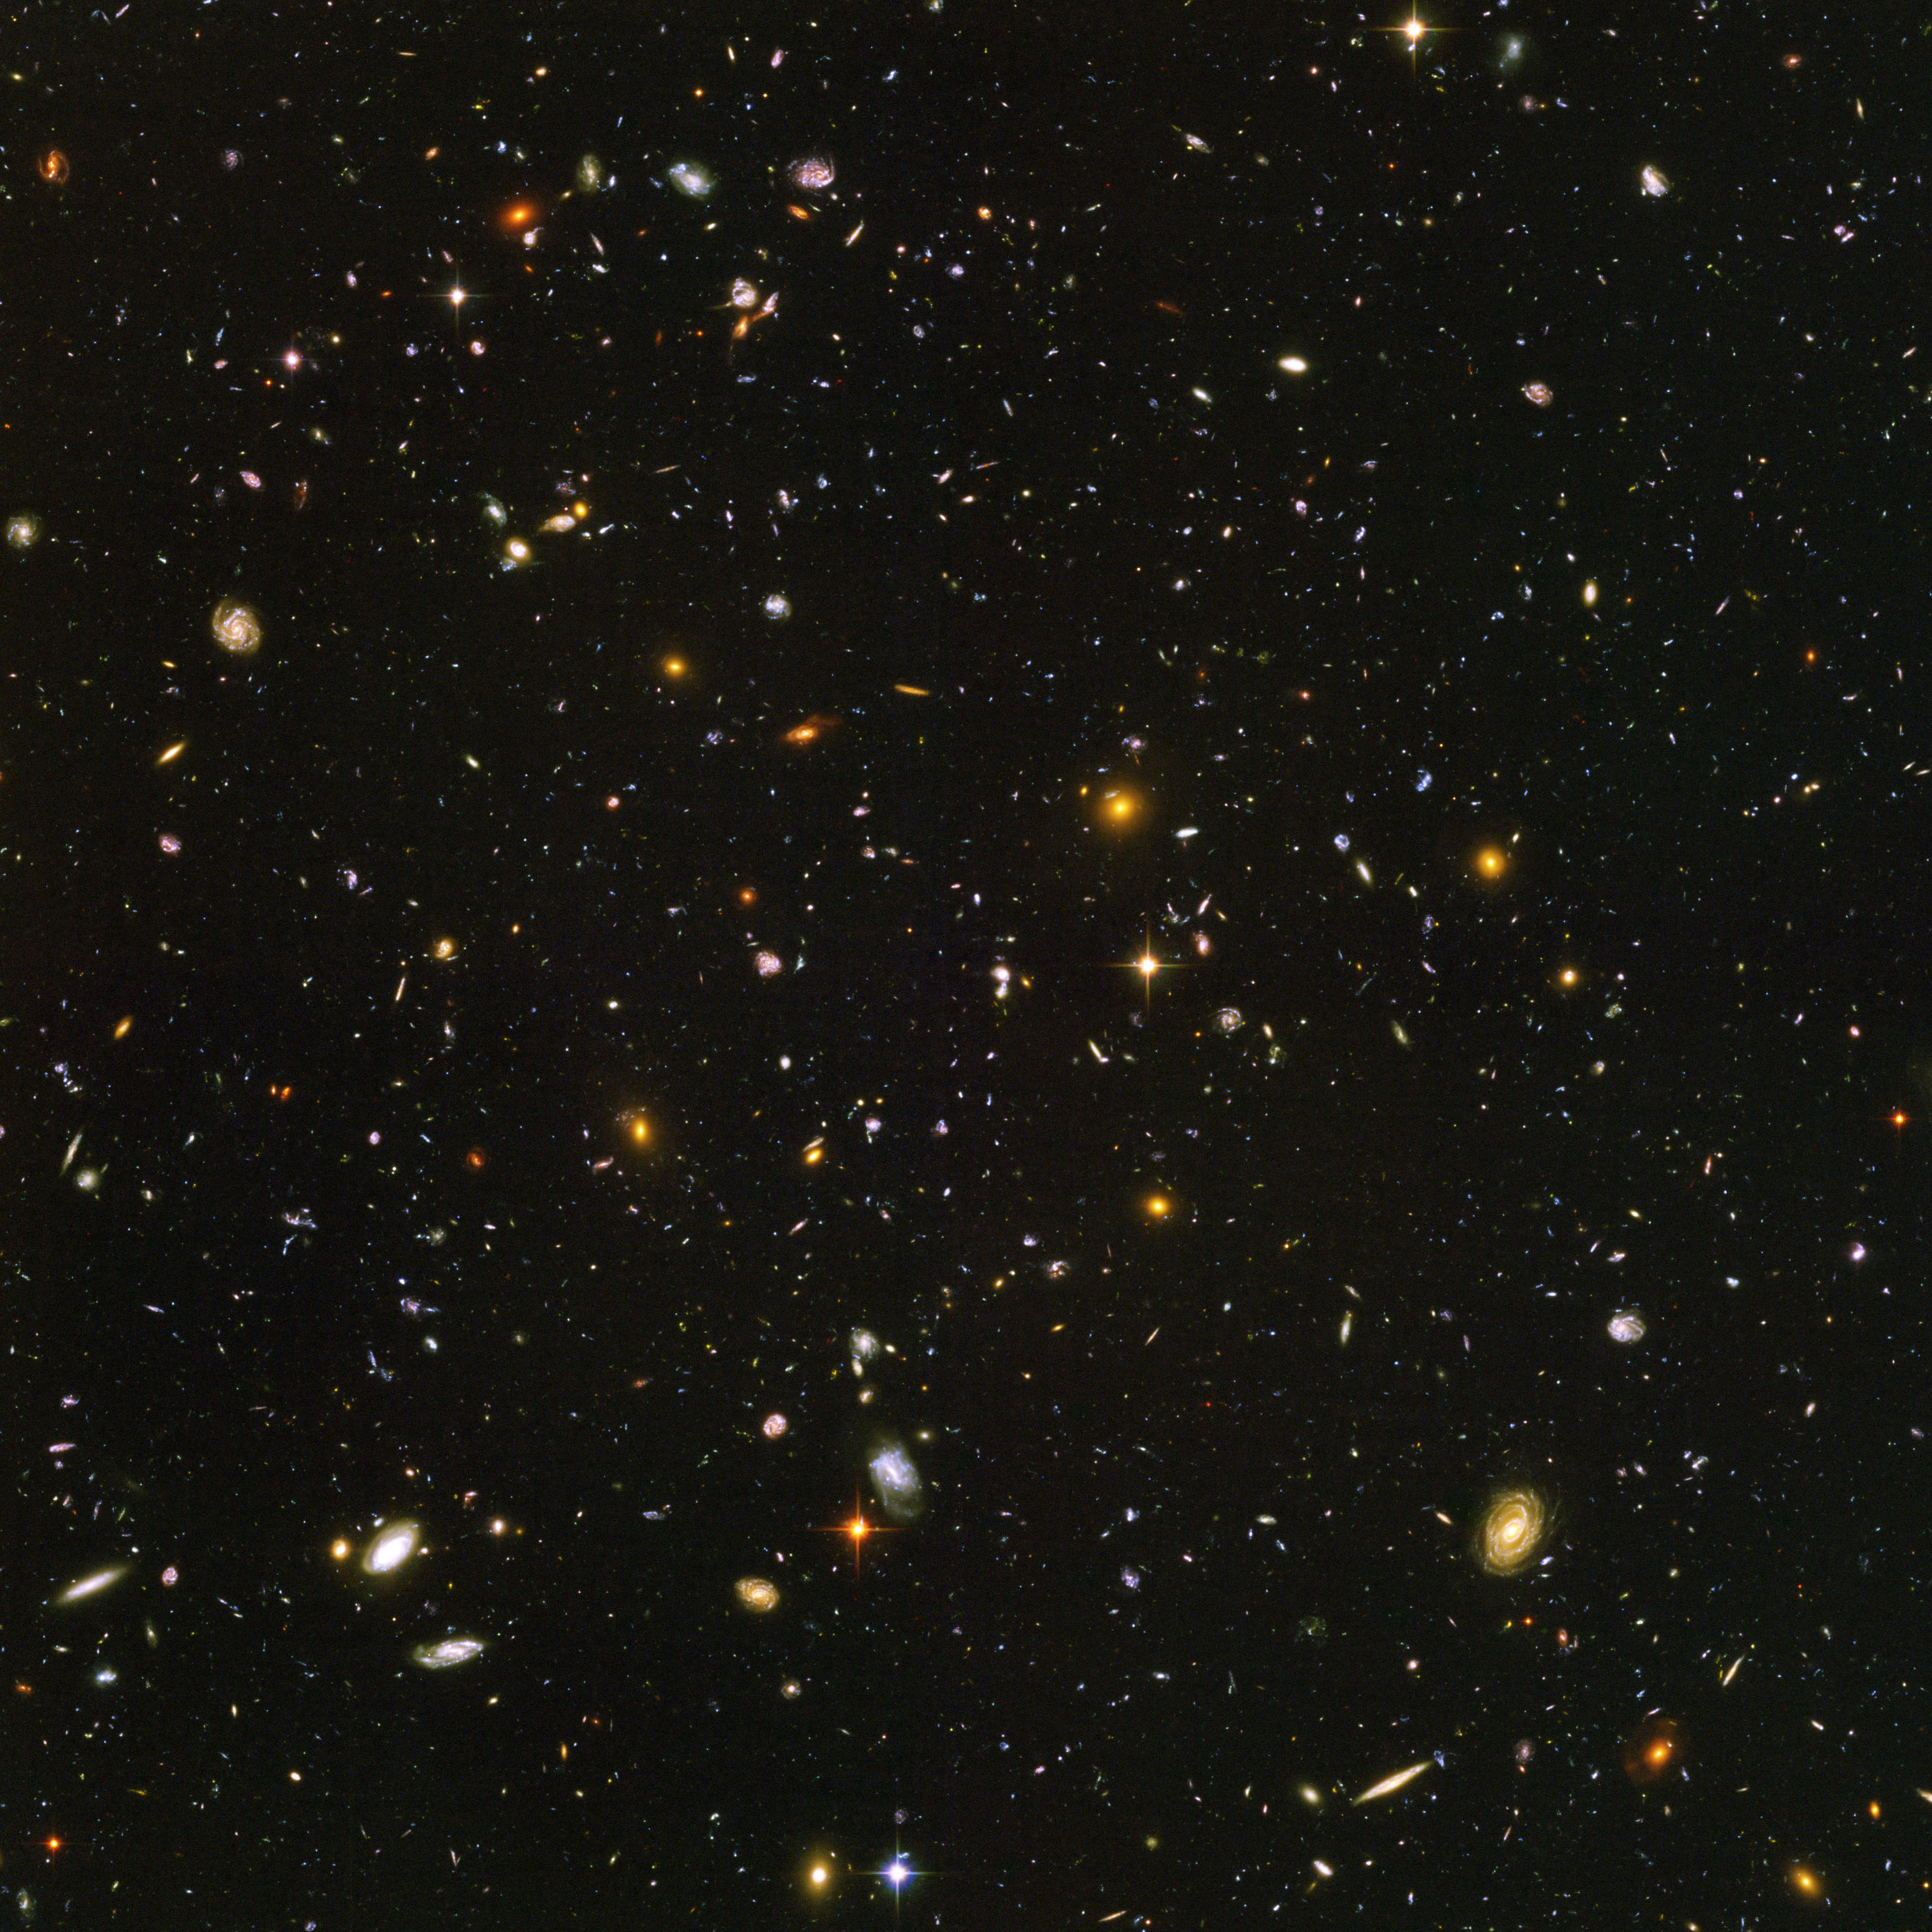
\includegraphics[width=0.8\textwidth]{UDF_half.jpg}
    \end{center}
    {\normalsize Hubble UDF}
}

\frame
{
    \begin{center}
        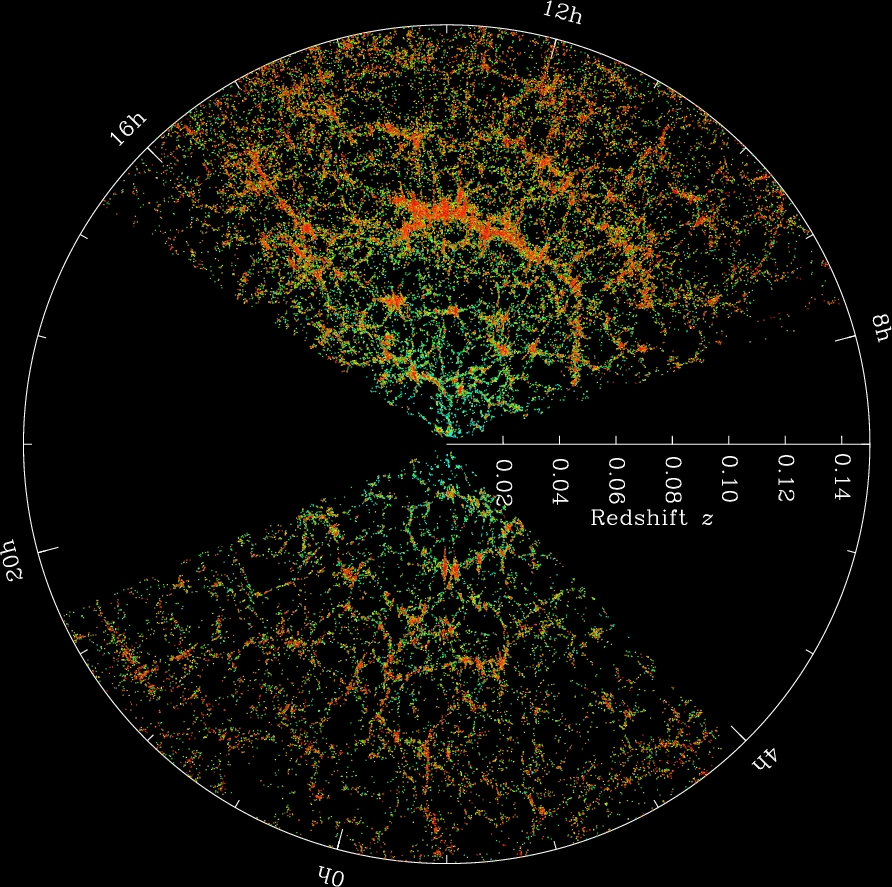
\includegraphics[height=0.9\textheight]{orangepie.jpg}
    \end{center}
    {\normalsize SDSS Galaxy Locations (M. Blanton)}
}



\begin{comment}
\frame
{

    \frametitle{What is the history of the universe?}

    \setbeamerfont*{itemize/enumerate body}{size=\small}

    \begin{columns}
        \begin{column}{0.5\textwidth}
            \begin{itemize}

                \item The universe is expanding

                \item Long ago the universe
                    was extremely hot and dense

                \item The Cosmic Microwave Background (CMB) is the relic light from
                    a few hundred thousand years after the big bang

                \item All the structure we see today must have grown from the
                    kind of fluctuations seen in this map, under the influence
                    of gravity.
                    
                \item Can we predict what we see today from CMB observations?

            \end{itemize}
        \end{column}
        \begin{column}{0.5\textwidth}
            \begin{center}
                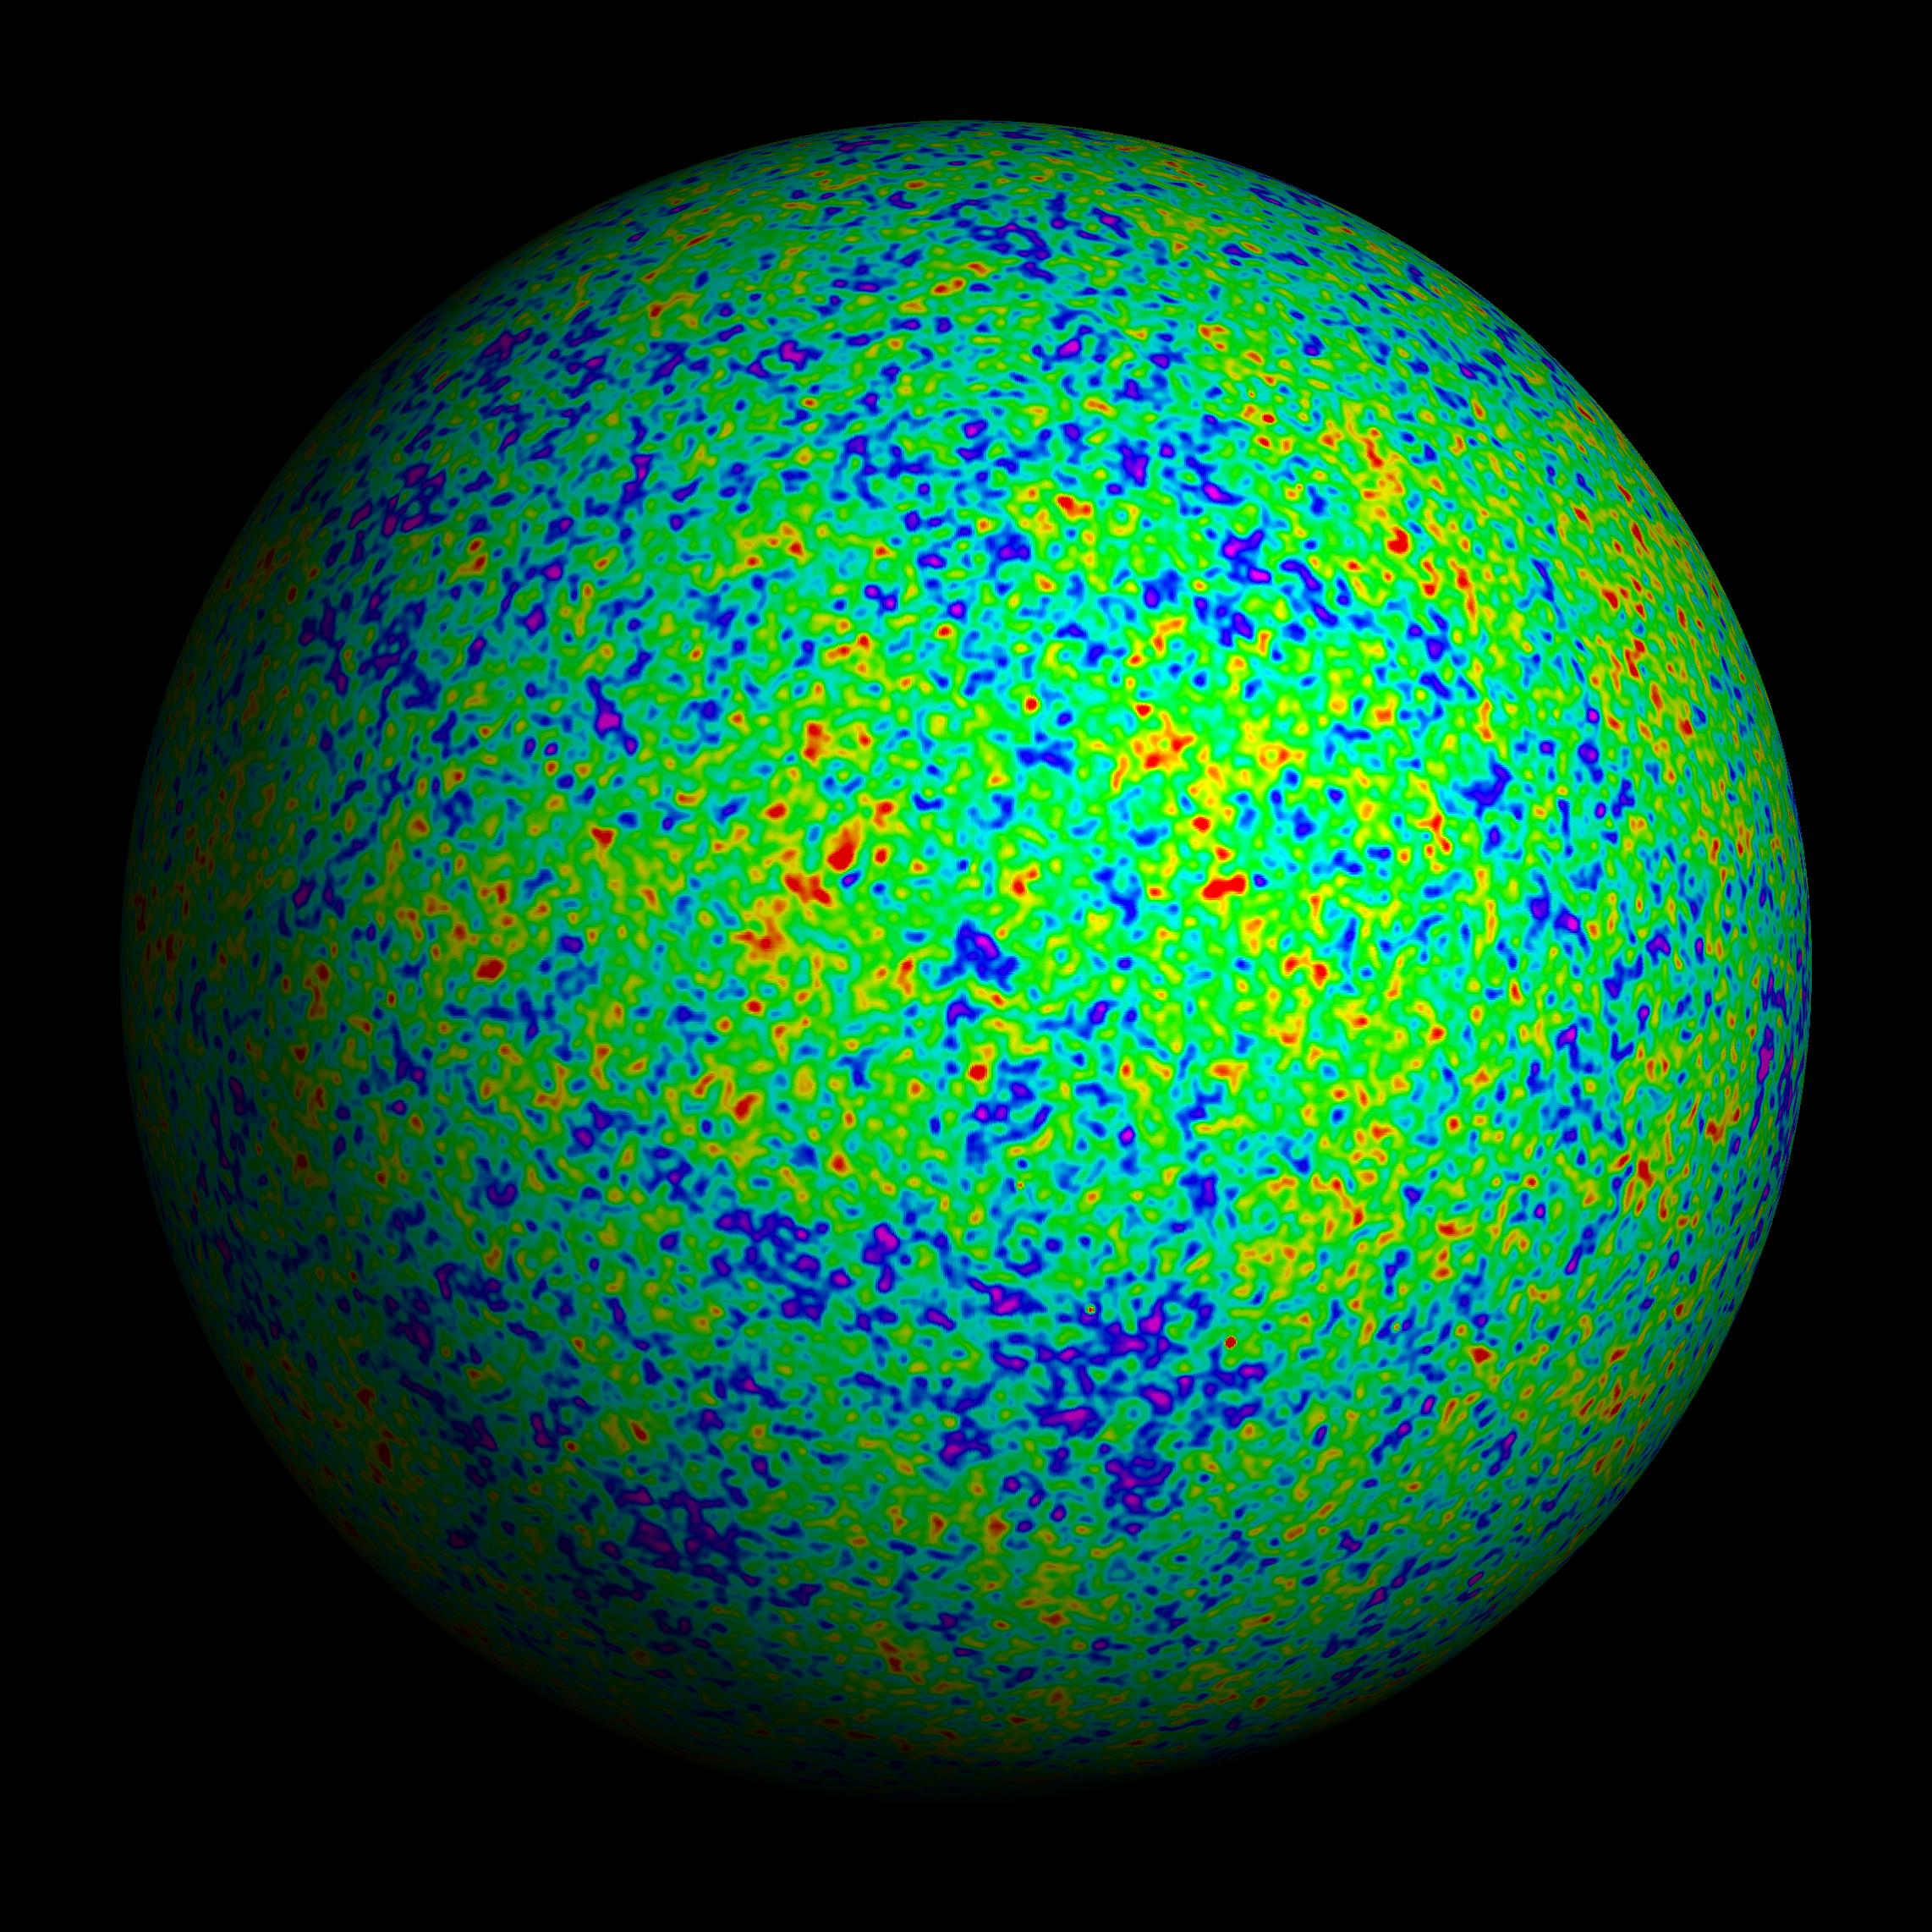
\includegraphics[width=\textwidth]{wiener3yr_map_2284x2284.jpg}
            \end{center}
        \end{column}
    \end{columns}


}


\frame
{
    \begin{center}
        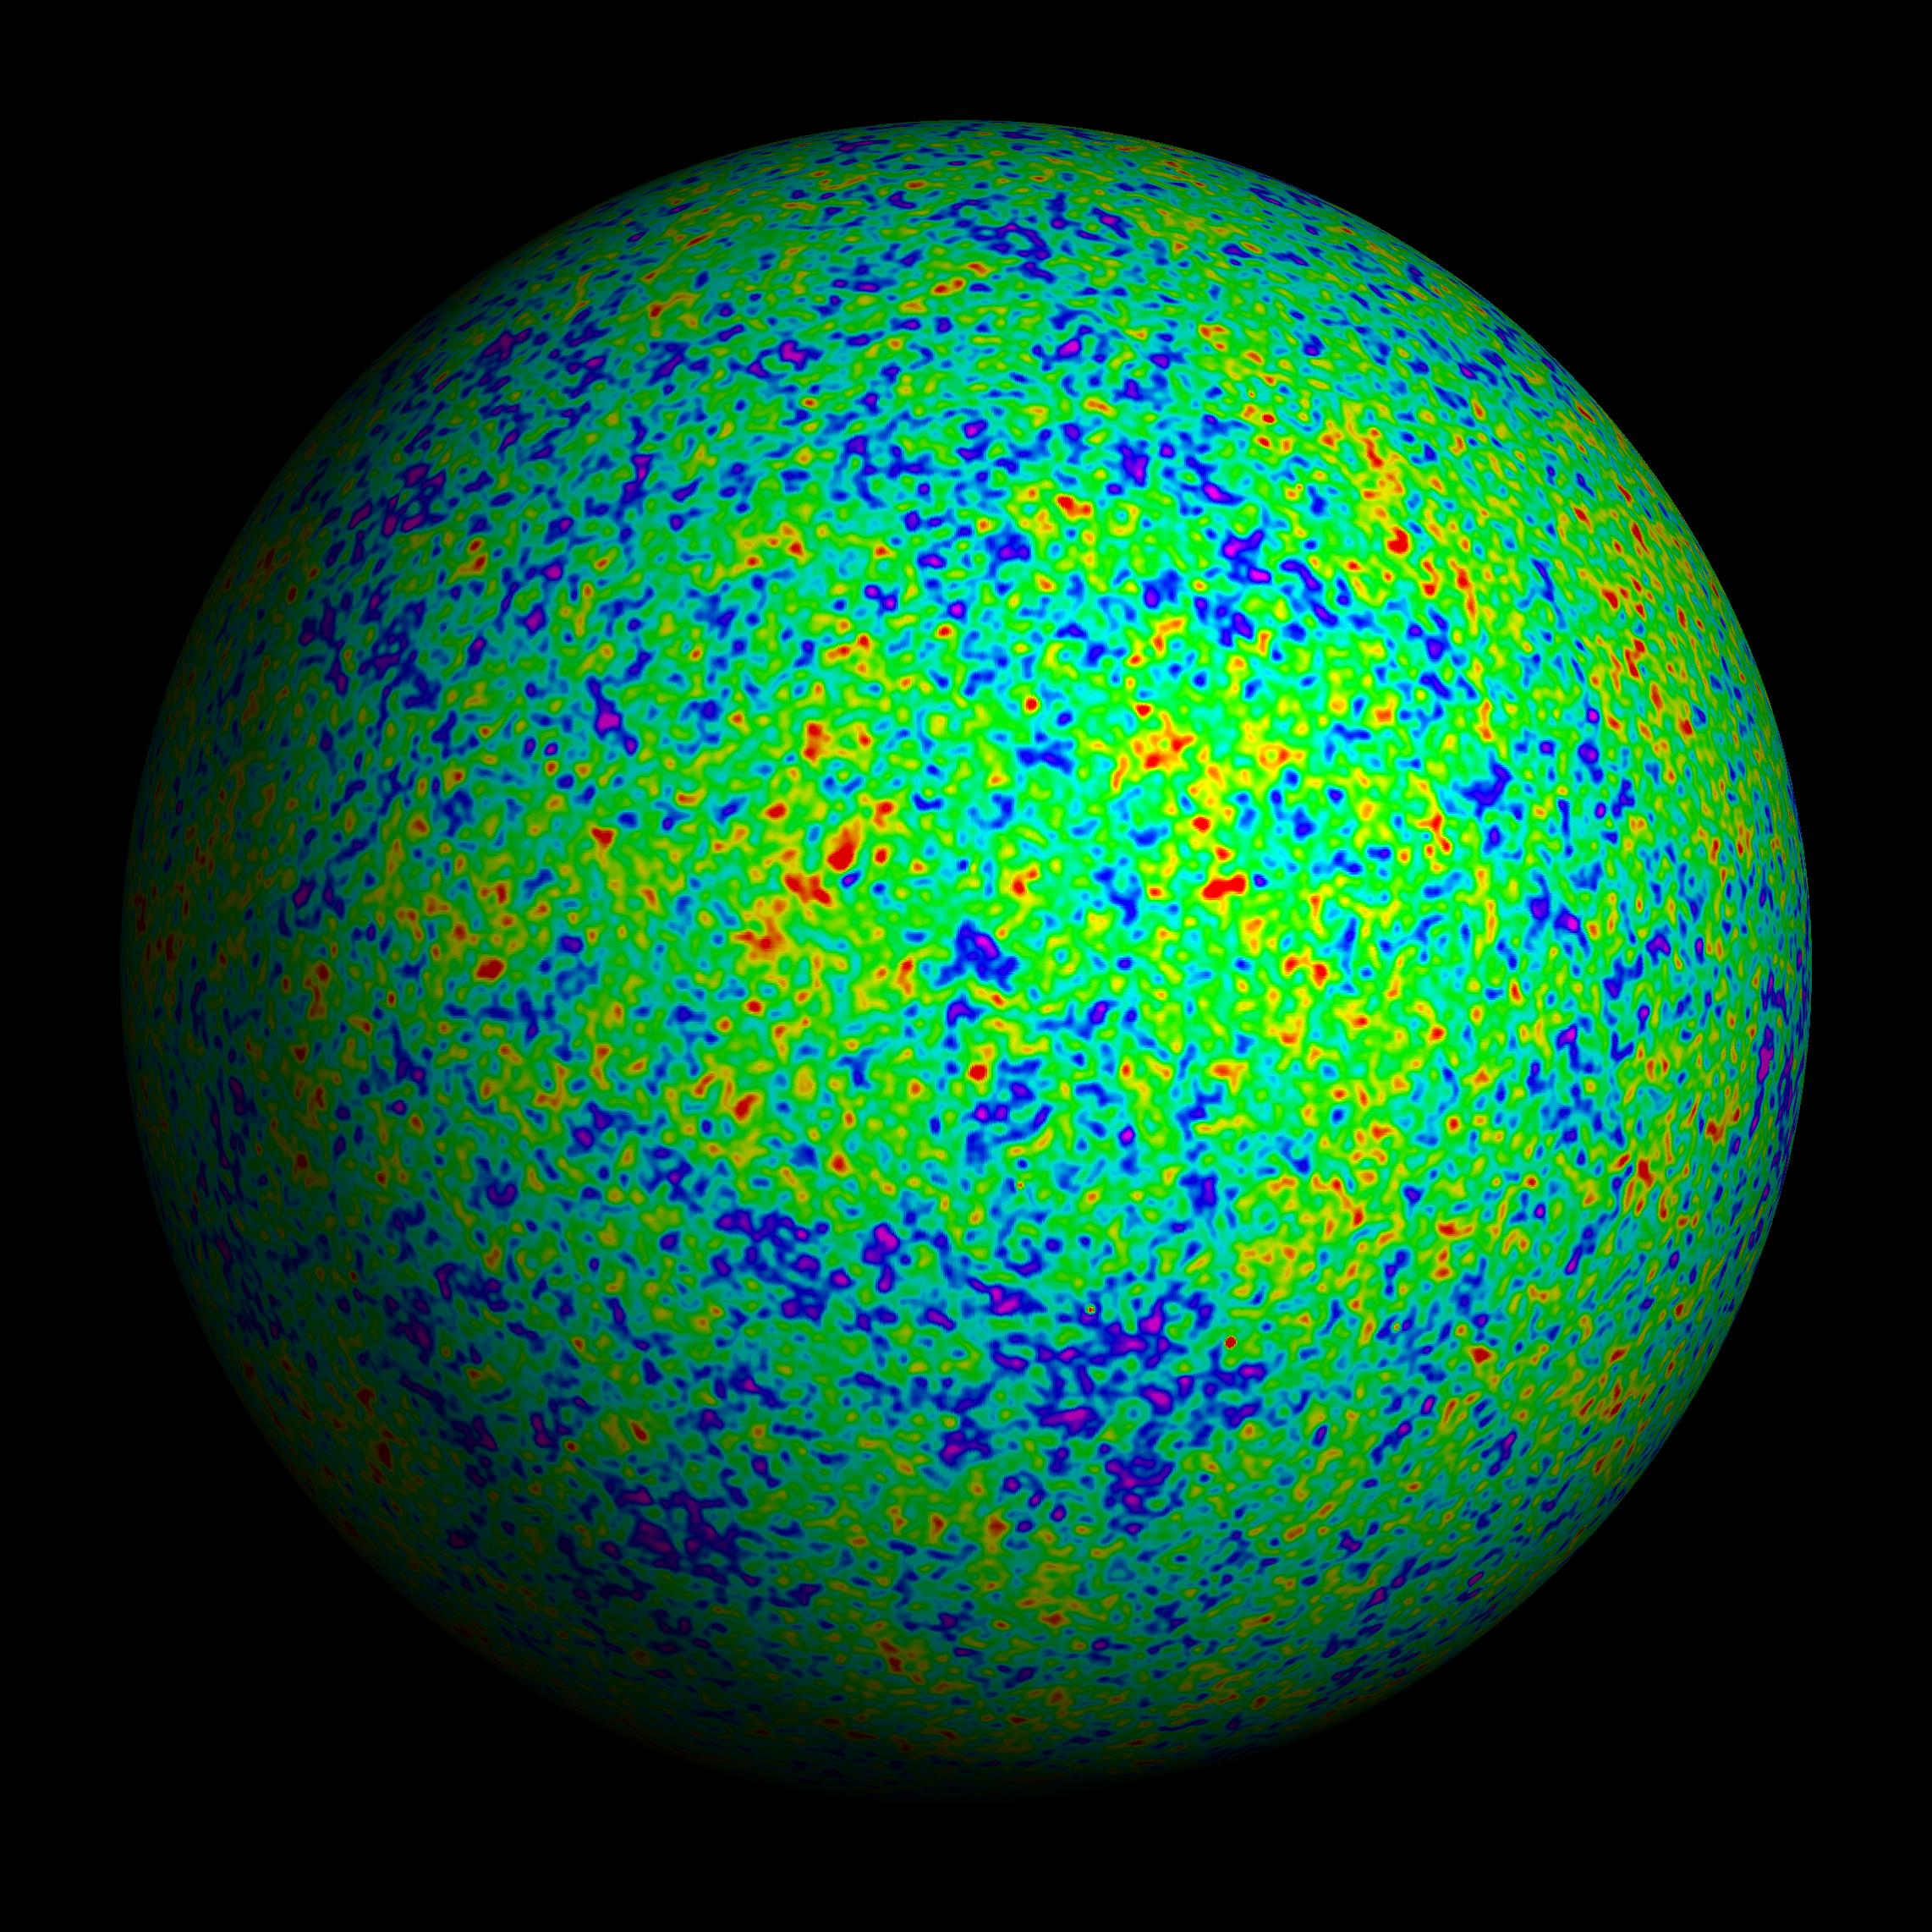
\includegraphics[width=0.75\textwidth]{wiener3yr_map_2284x2284.jpg}
    \end{center}
    {\normalsize Image of the universe 300,000 years after the big bang (Tegmark, WMAP)}
}

\end{comment}

\frame
{

    \frametitle{What is the history of the universe?}

    \setbeamerfont*{itemize/enumerate body}{size=\small}

    \begin{columns}
        \begin{column}{0.5\textwidth}
            \begin{itemize}


                \item The universe is expanding.  Galaxies farther away from
                    us moving away faster and their light is redshifted
                    
                \item That is our view, but you would see the same thing
                    from any other galaxy in the universe

                \item We can get an estimate of distance from the
                    velocity/redshift.
                    
                \item Because we see these galaxies as they were far back in
                    time, the history is tied to the question of where things
                    are.

            \end{itemize}
        \end{column}
        \begin{column}{0.5\textwidth}
            \begin{center}
                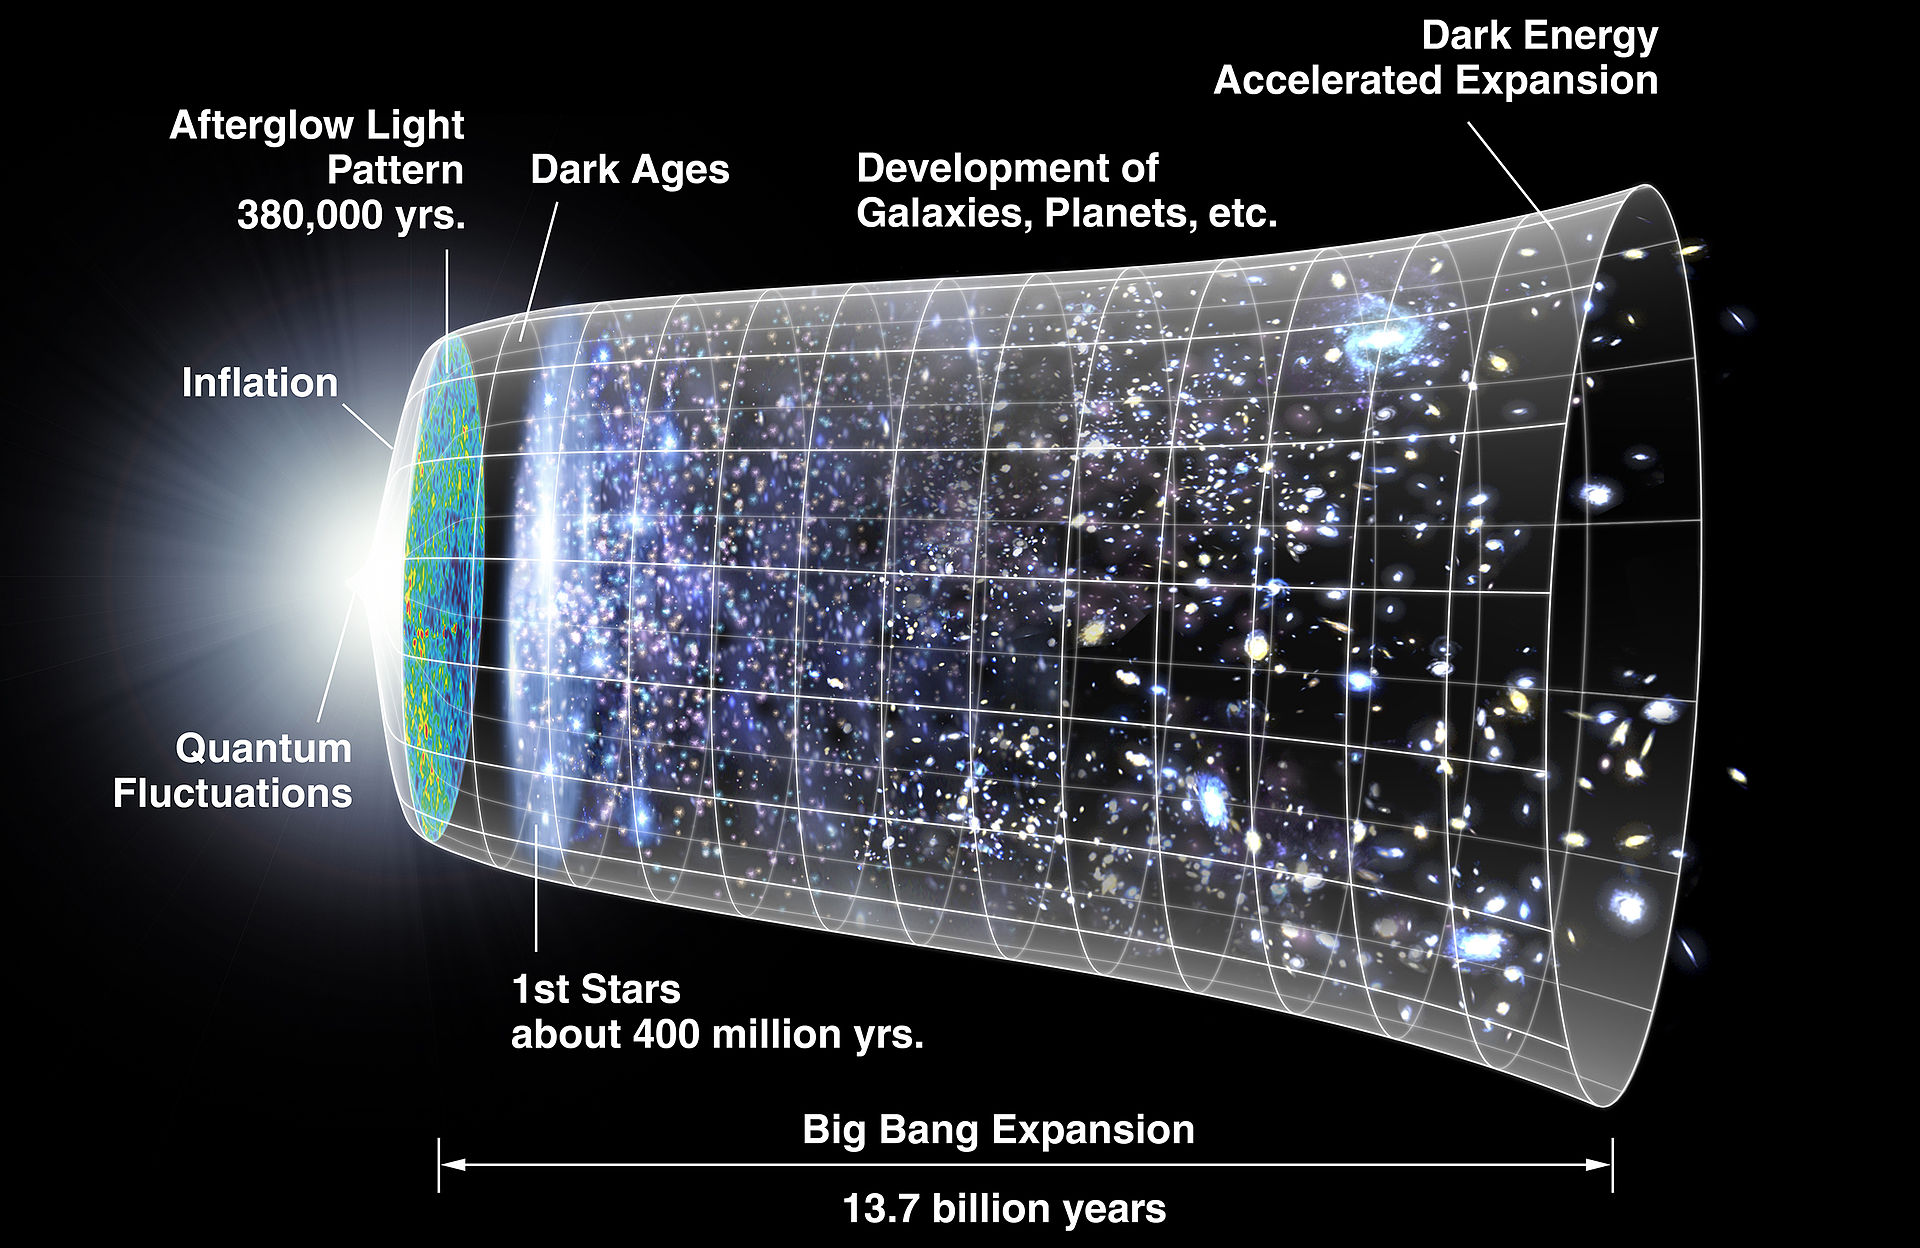
\includegraphics[width=\textwidth]{CMB_Timeline300_no_WMAP.jpg}
            \end{center}
            
        \end{column}
    \end{columns}


}

\frame
{

    \frametitle{What is the history of the universe?}

    \setbeamerfont*{itemize/enumerate body}{size=\small}

    \begin{columns}
        \begin{column}{0.5\textwidth}
            \begin{itemize}


                \item We expected the expansion to decelerate. 

                \item The measurements indicated it {\em did} decelerate for a
                    long time, but then began to accelerate!
                    
                \item This mystery is called Dark Energy 
                    

            \end{itemize}
        \end{column}
        \begin{column}{0.5\textwidth}
            \begin{center}
                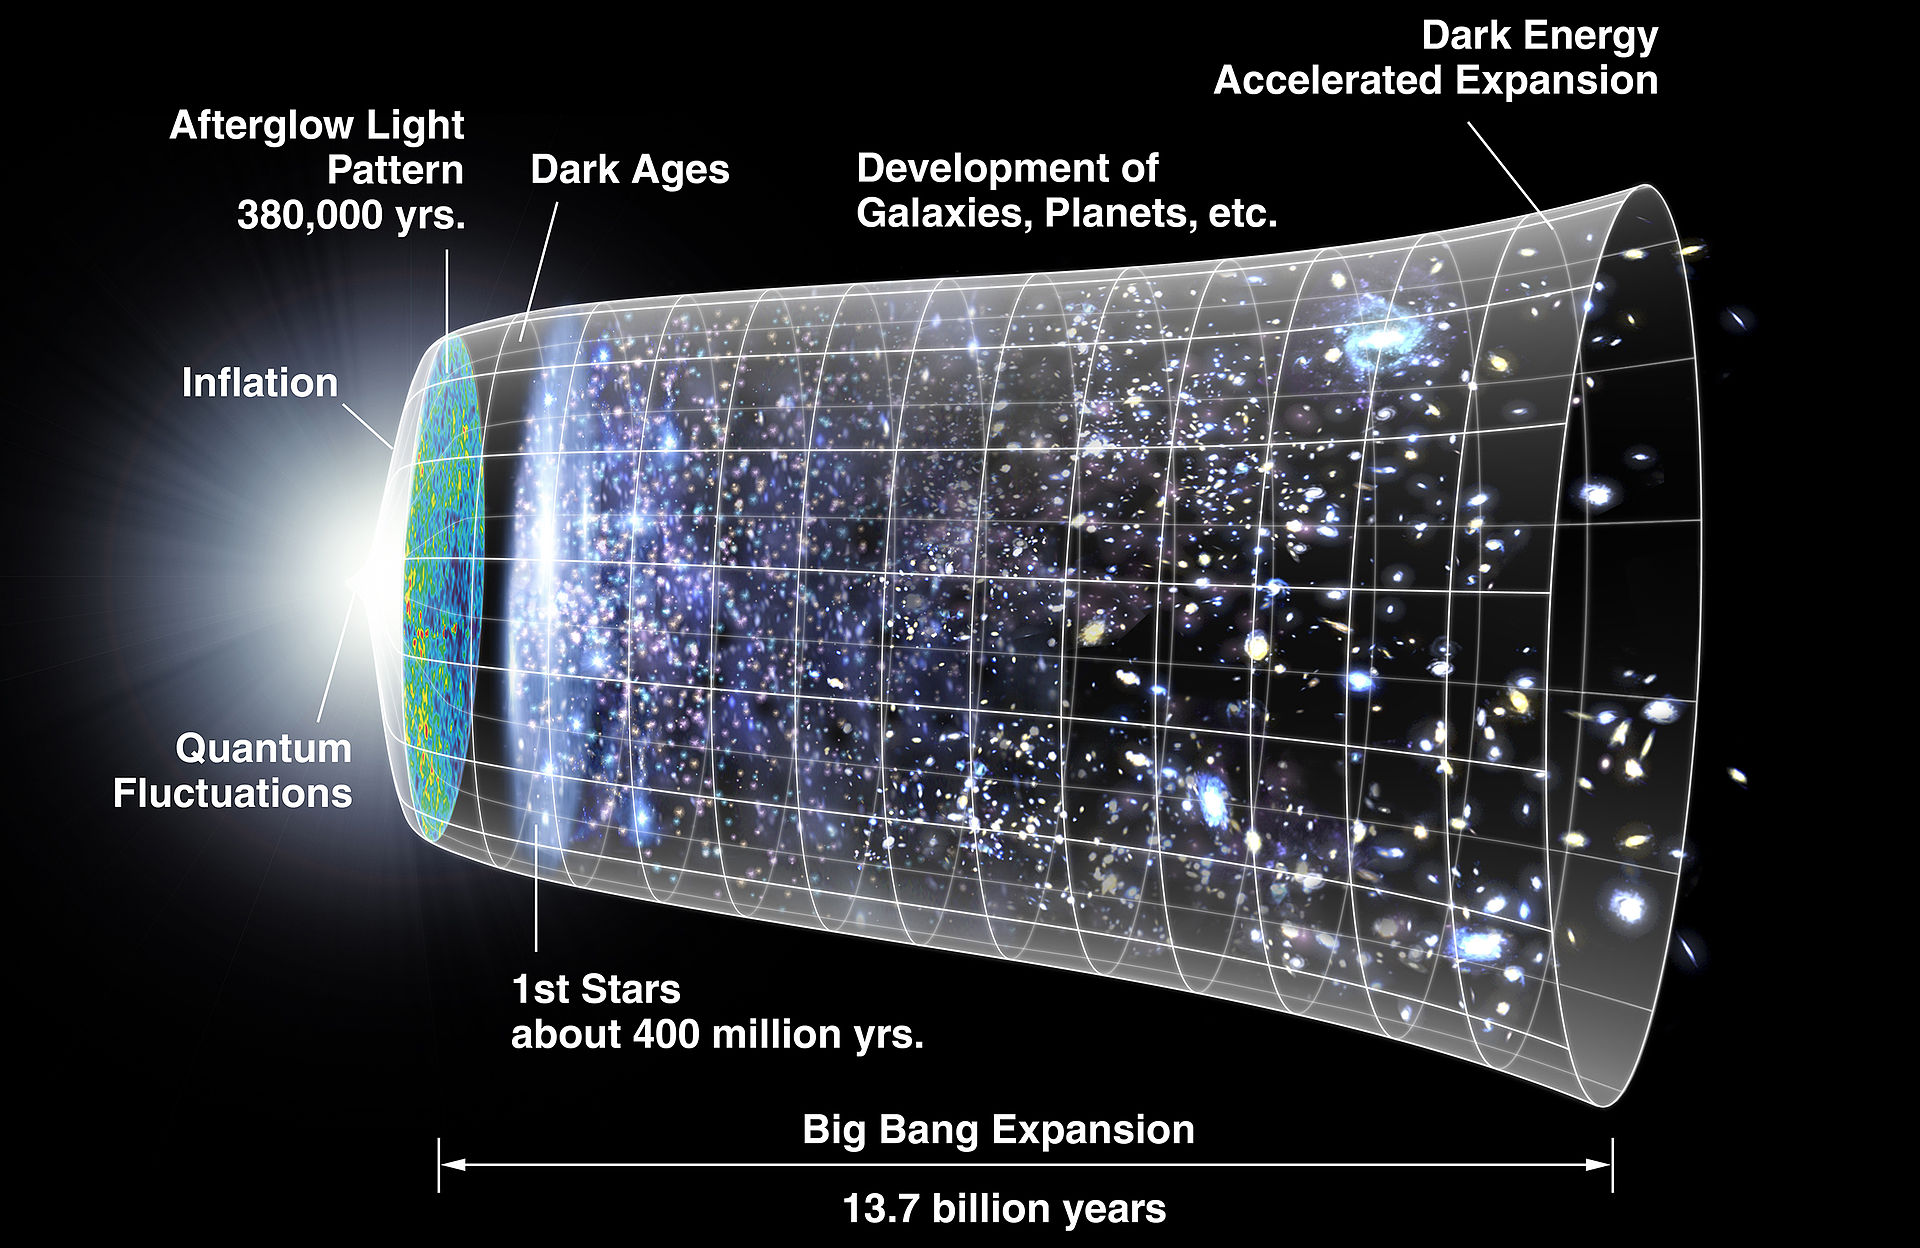
\includegraphics[width=\textwidth]{CMB_Timeline300_no_WMAP.jpg}
            \end{center}
            
        \end{column}
    \end{columns}


}

\frame
{
    \begin{center}
        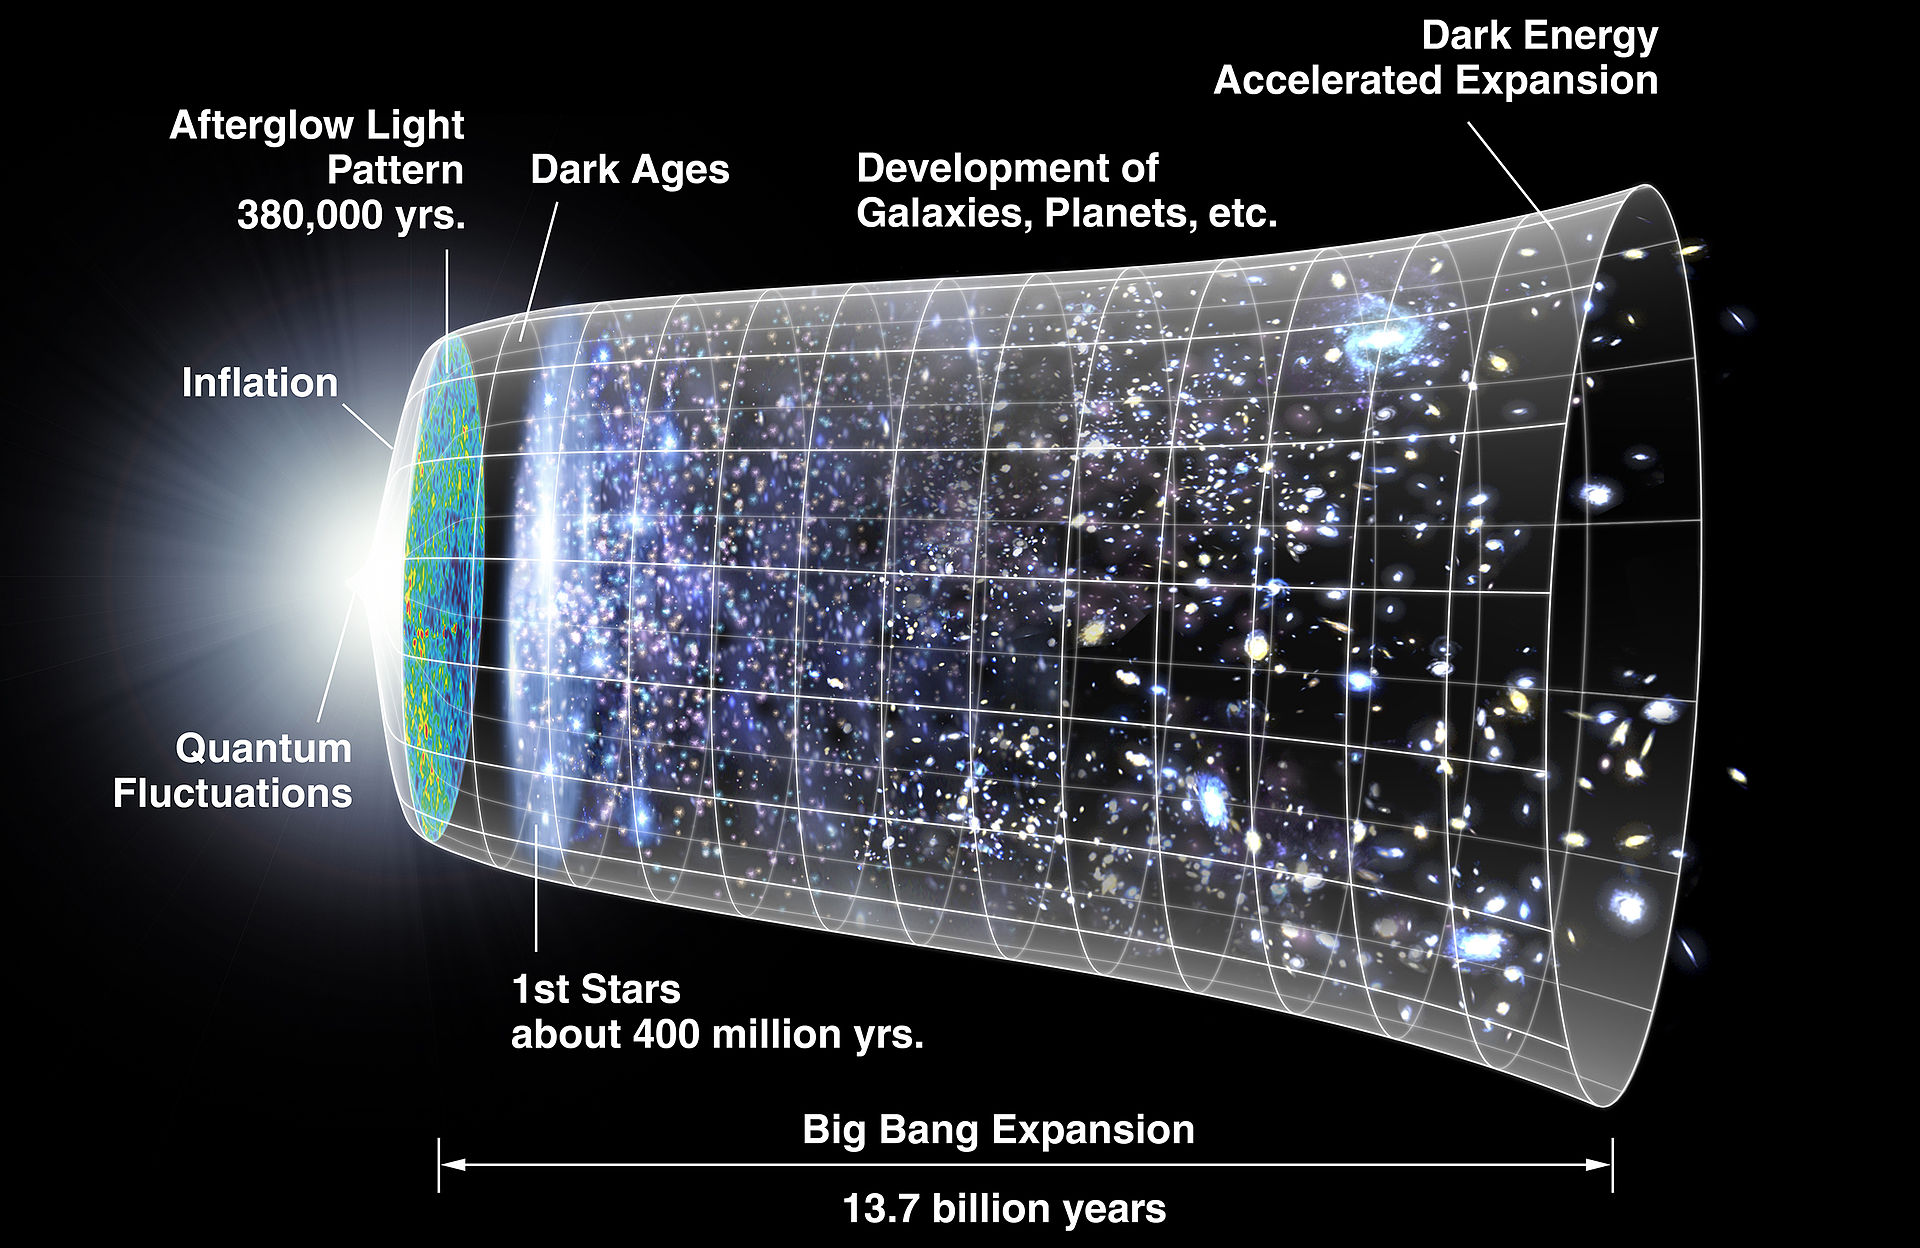
\includegraphics[width=0.9\textwidth]{CMB_Timeline300_no_WMAP.jpg}
    \end{center}
    {\normalsize Model of the expansion history (WMAP)}
}


\frame
{

    \frametitle{The Big Mysteries We Want to Study}

    \setbeamerfont*{itemize/enumerate body}{size=\small}

    \begin{columns}
        \begin{column}{0.5\textwidth}
            \begin{itemize}


                \item What is the Dark Matter?  Where is it and how much
                    is there?

                \item What is the Dark Energy?  What are its propeties and how
                    much is there?

            \end{itemize}
        \end{column}
        \begin{column}{0.5\textwidth}
            \begin{center}
                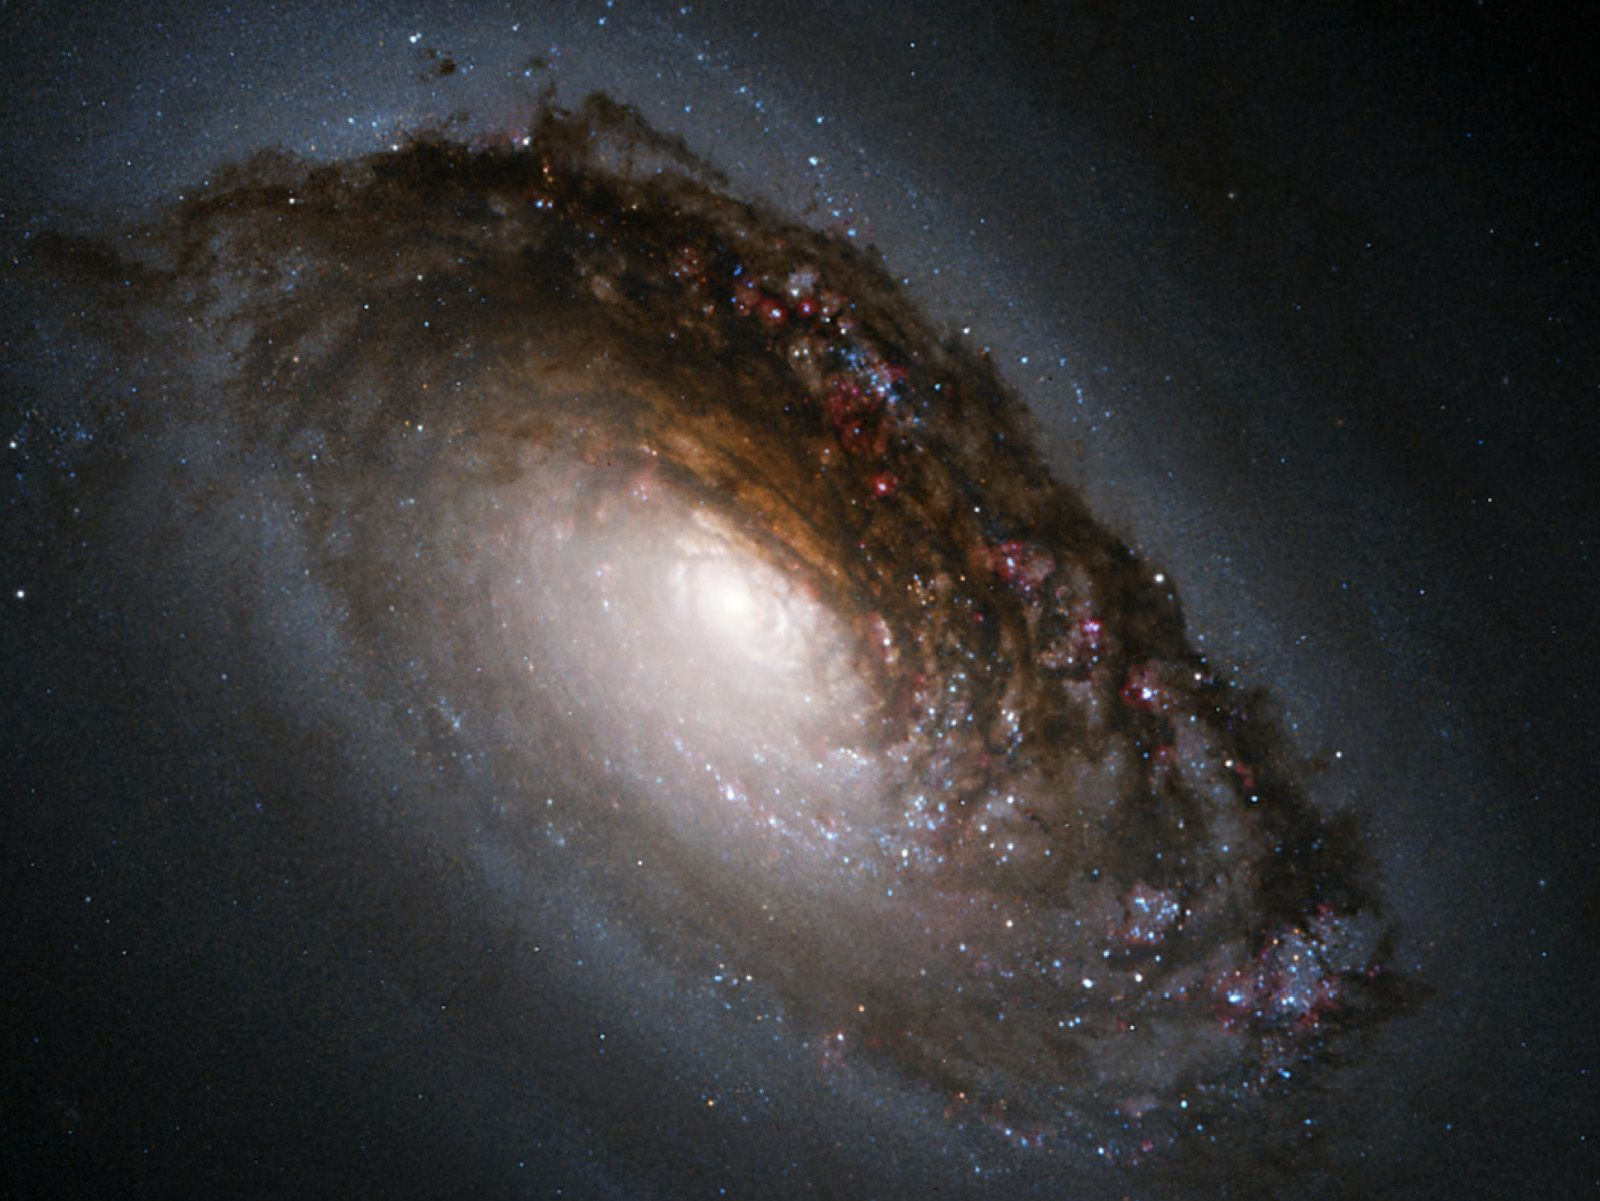
\includegraphics[width=\textwidth]{m64-black-eye-galaxy.jpg}
                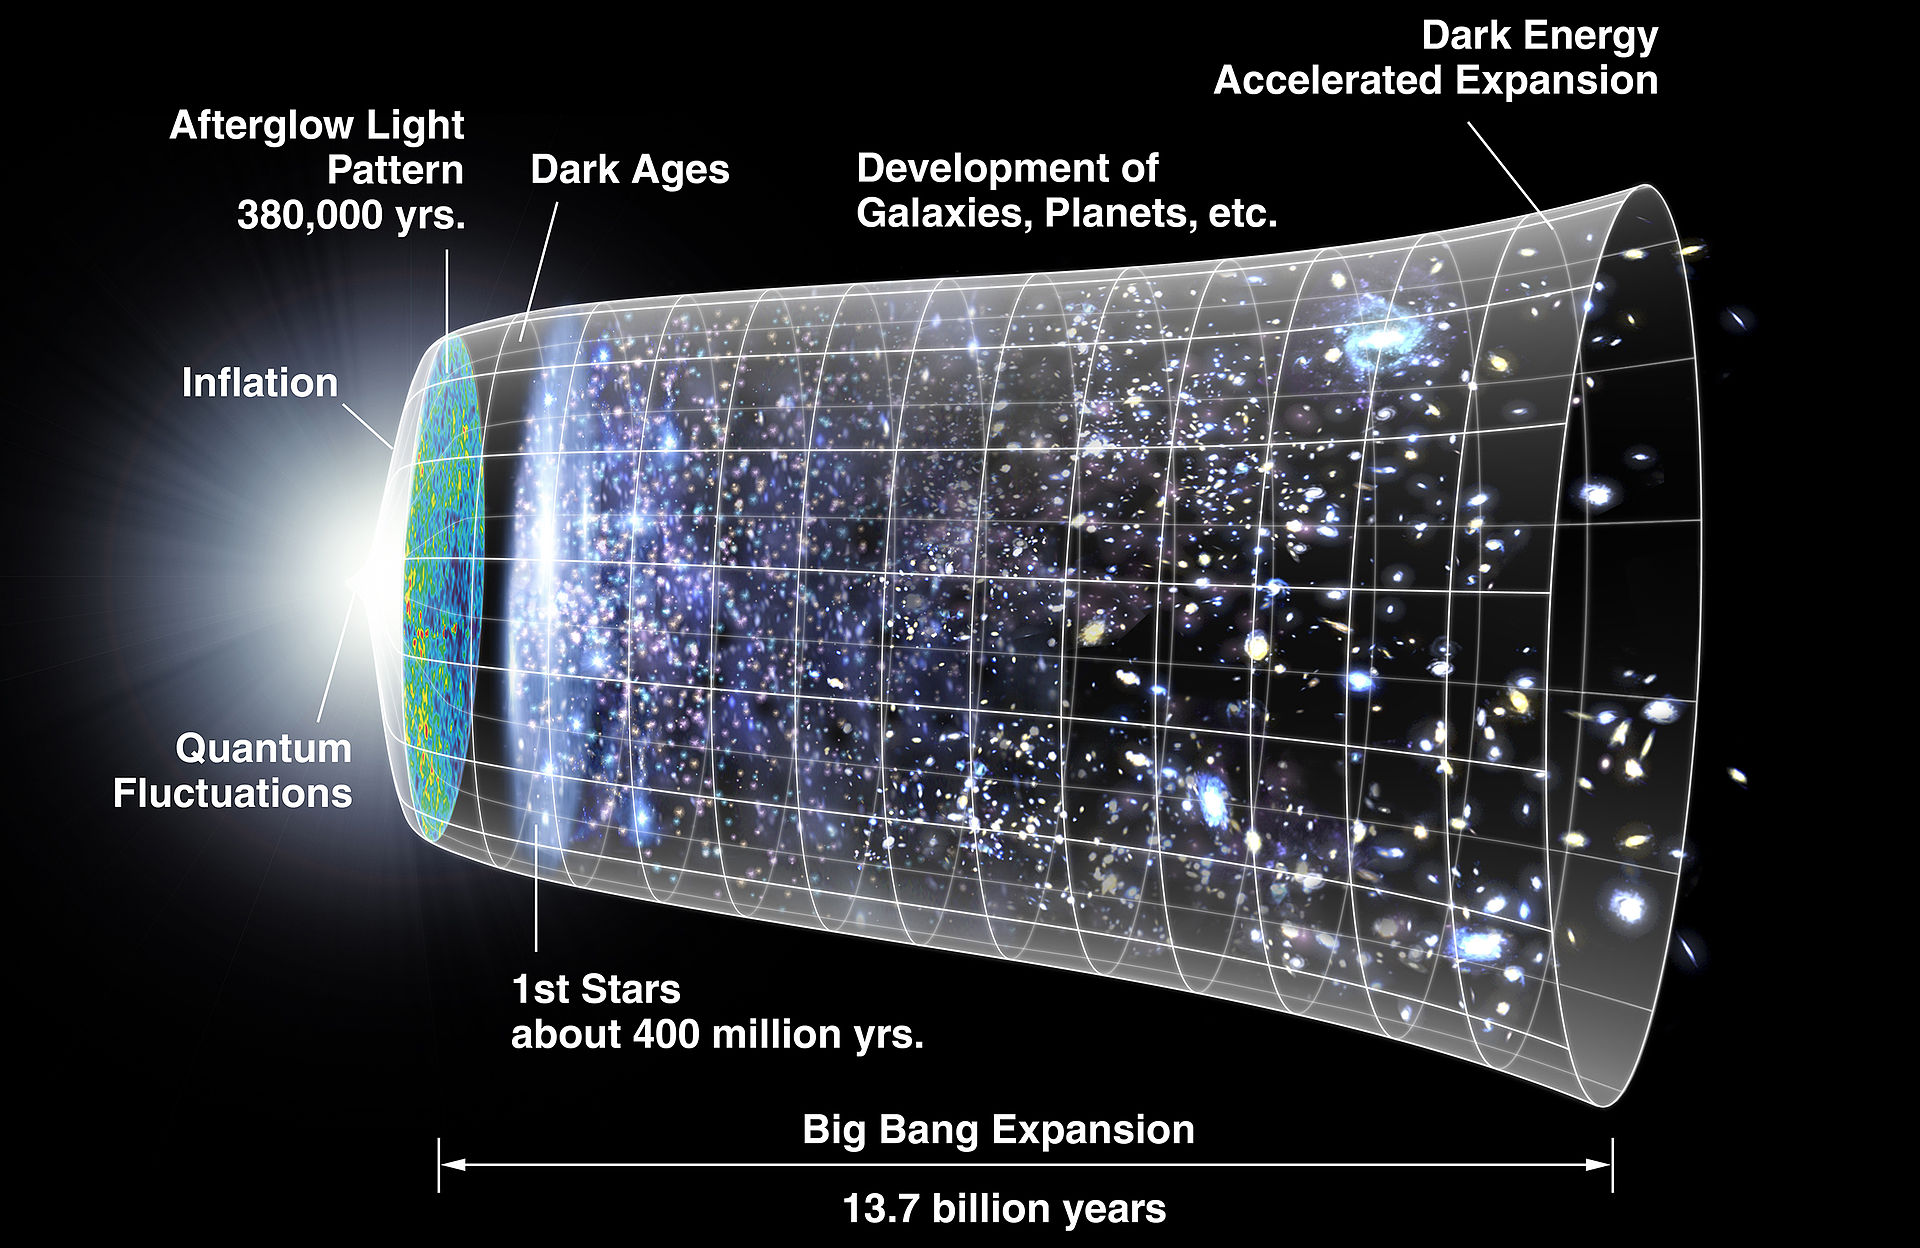
\includegraphics[width=\textwidth]{CMB_Timeline300_no_WMAP.jpg}
            \end{center}
            
        \end{column}
    \end{columns}


}



\frame
{

    {\huge Gravitational Lensing}

}

\frame
{
            \begin{center}
                \includegraphics[width=\textwidth]{A_Horseshoe_Einstein_Ring_from_Hubble.JPG}
            \end{center}
            {\tiny HST/NASA}

    
}
\frame
{
            \begin{center}
                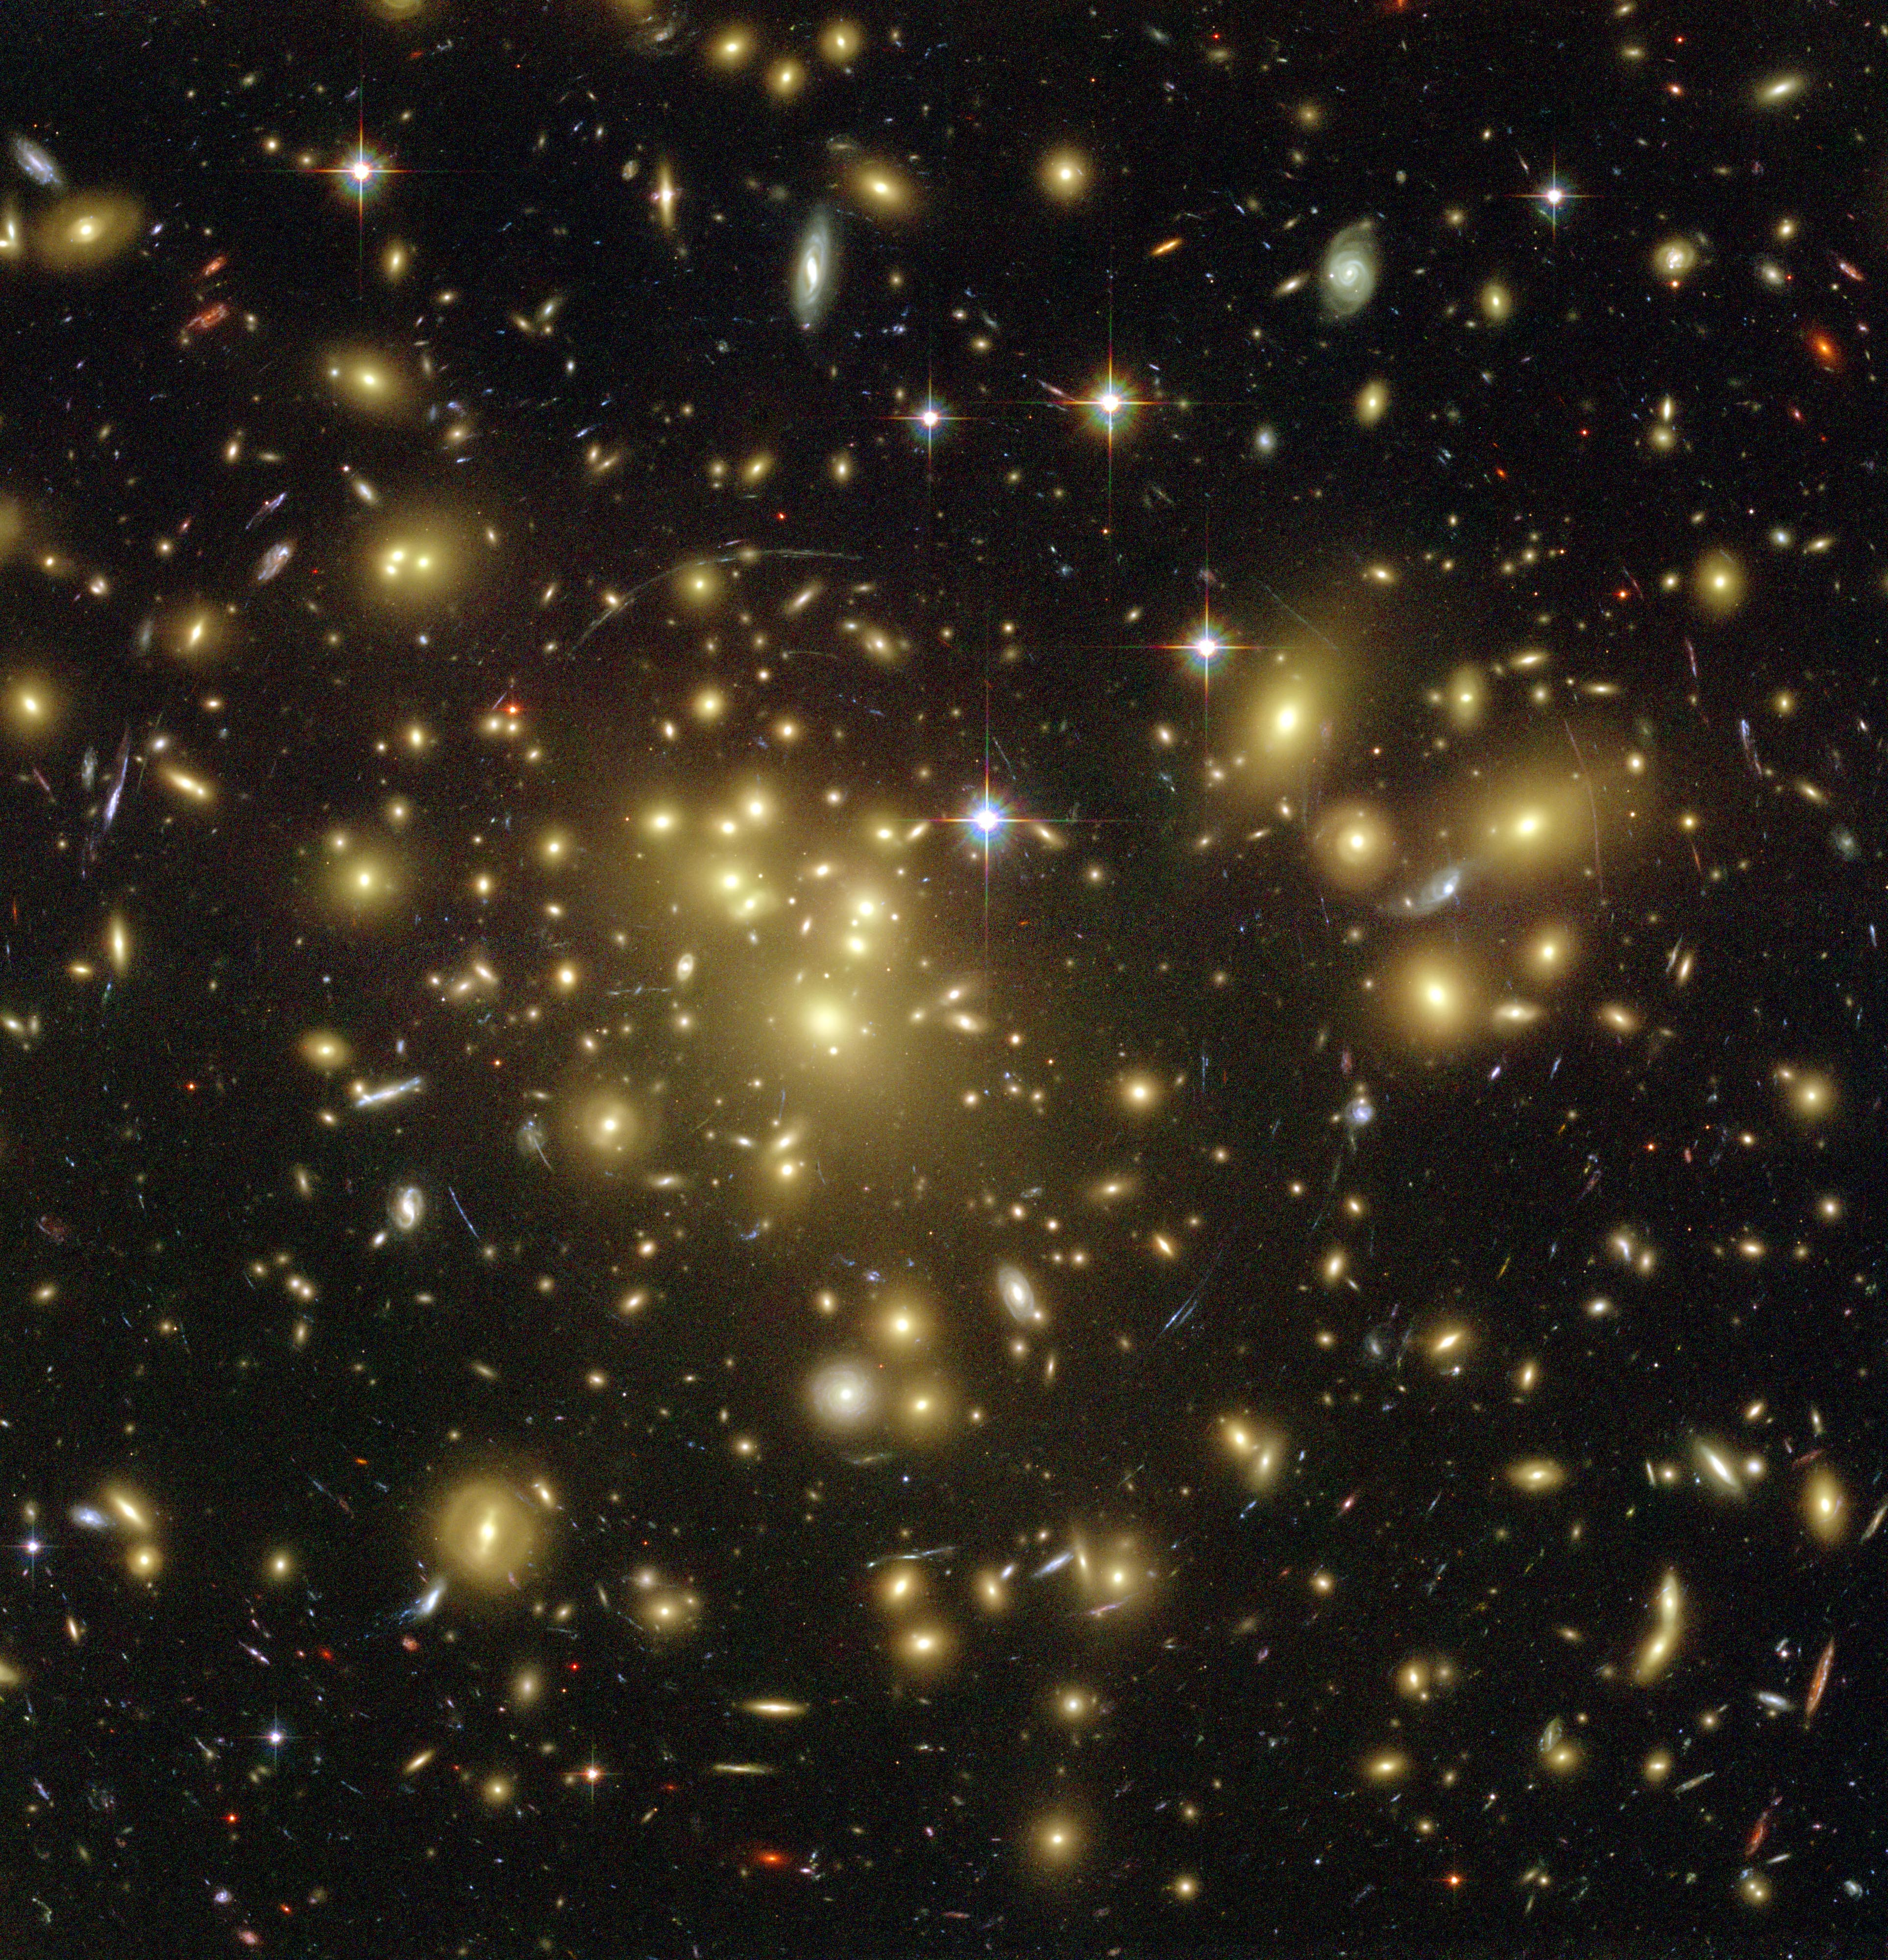
\includegraphics[height=\textheight]{abell-1689-hubble.jpg}
            \end{center}
            {\tiny HST/NASA}

    
}

\frame
{

    \frametitle{Gravitational Lensing}

    \setbeamerfont*{itemize/enumerate body}{size=\small}

    \begin{columns}
        \begin{column}{0.5\textwidth}
            \begin{itemize}

                \item Gravitational lensing is the apparent bending of light
                    rays as they pass massive objects


            \end{itemize}
        \end{column}
        \begin{column}{0.5\textwidth}
            \begin{center}
                
\includegraphics[width=\textwidth]{lens_geometry_invert.pdf}
            \end{center}

            
        \end{column}
    \end{columns}


}

\frame
{
            \begin{center}
                
\includegraphics[width=0.85\textwidth]{lens_geometry_invert.pdf}
            \end{center}
}

\frame
{

    \frametitle{Gravitational Lensing Compared To Ordinary Lensing}

    \setbeamerfont*{itemize/enumerate body}{size=\small}

    \begin{columns}
        \begin{column}{0.5\textwidth}
            \begin{itemize}

                \item Similar in that the magnification depends on the
                    curvature of the lens and the distances.
                    \begin{align}
                        \frac{1}{o} + \frac{1}{i} &= \frac{1}{f} \nonumber \\
                        m &= \frac{i}{o} \nonumber
                    \end{align}

            \end{itemize}
        \end{column}
        \begin{column}{0.5\textwidth}
            \begin{center}
                {\tiny Halliday and Resnick}
                \newline
                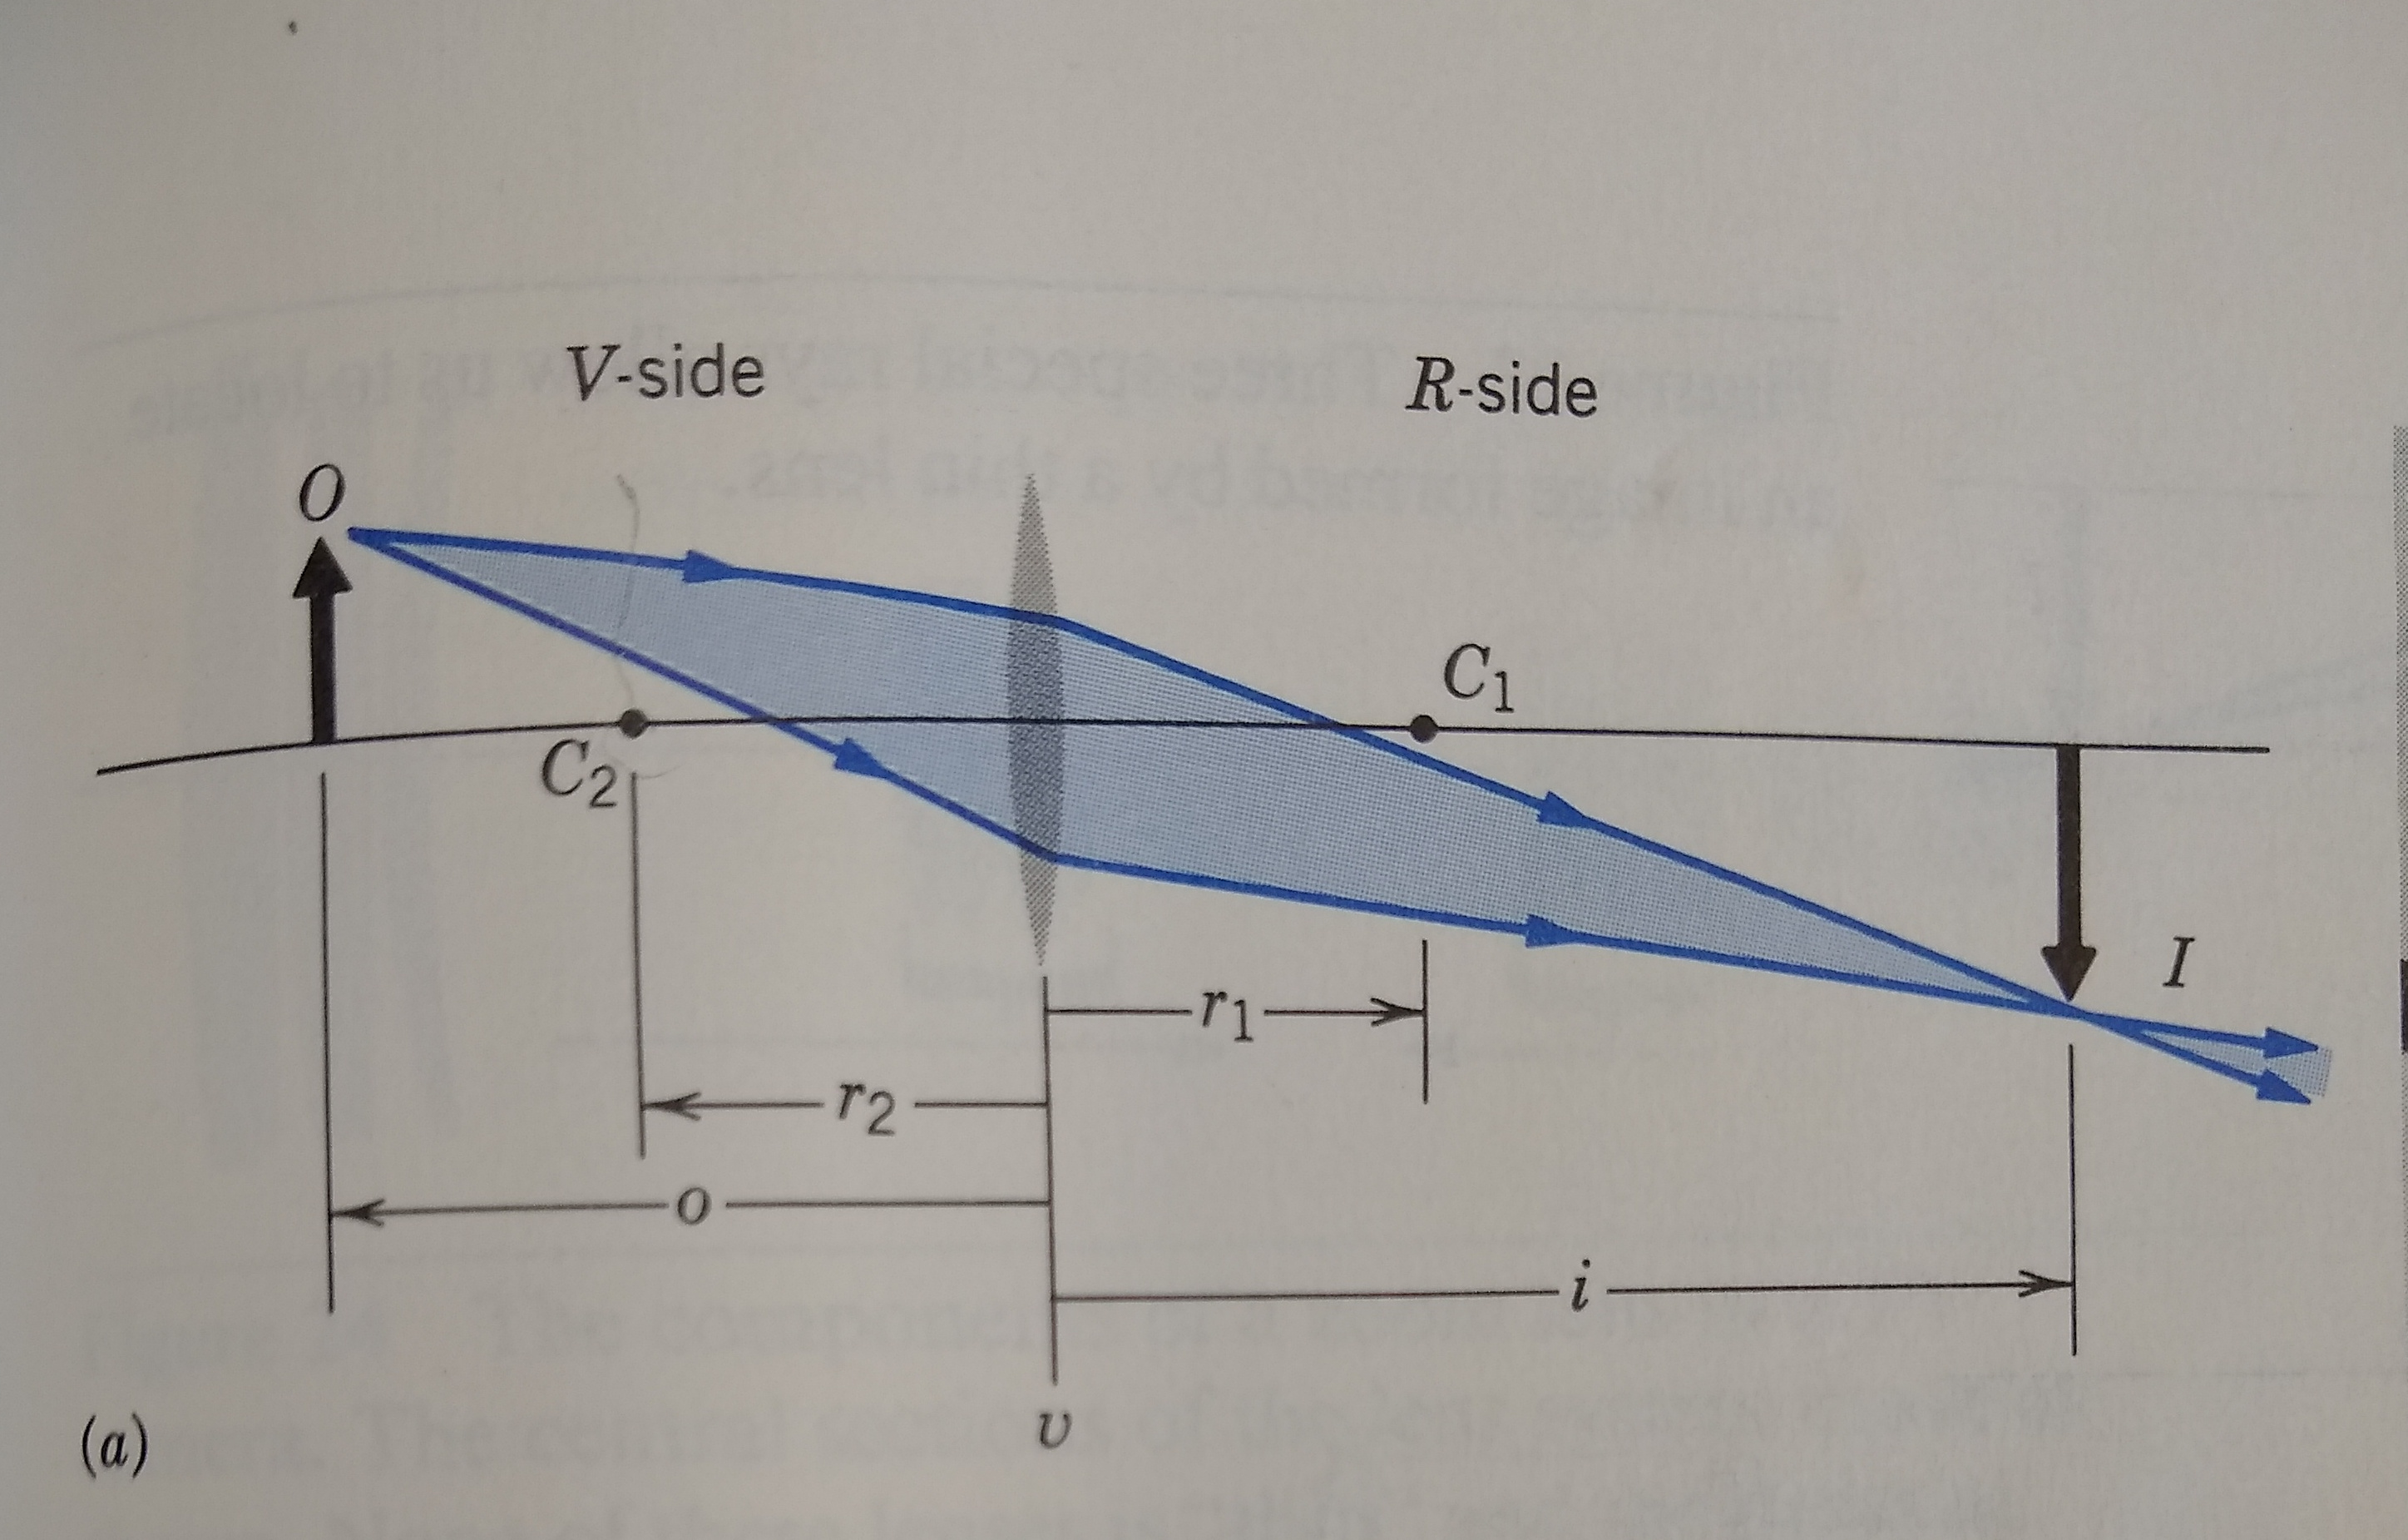
\includegraphics[width=\textwidth]{optics-halliday-resnick-crop.jpg}
                \newline
                
\includegraphics[width=\textwidth]{lens_geometry_invert.pdf}
            \end{center}

            
        \end{column}
    \end{columns}


}

\frame
{

    \frametitle{Gravitational Lensing Compared To Ordinary Lensing}

    \setbeamerfont*{itemize/enumerate body}{size=\small}

    \begin{columns}
        \begin{column}{0.5\textwidth}
            \begin{itemize}

                \item Difference:  The effect is strongest for paths that go
                    through the center of the lens (near the object)

                \item Difference: The image is not inverted

                \item Difference: Gravity is a long range force, so the effect
                    is present even for paths far from the lens.

                \item Difference: When the rays pass near the center,
                    you can see multiple images and rings even for simple lenses.

            \end{itemize}
        \end{column}
        \begin{column}{0.5\textwidth}
            \begin{center}
                {\tiny Halliday and Resnick}
                \newline
                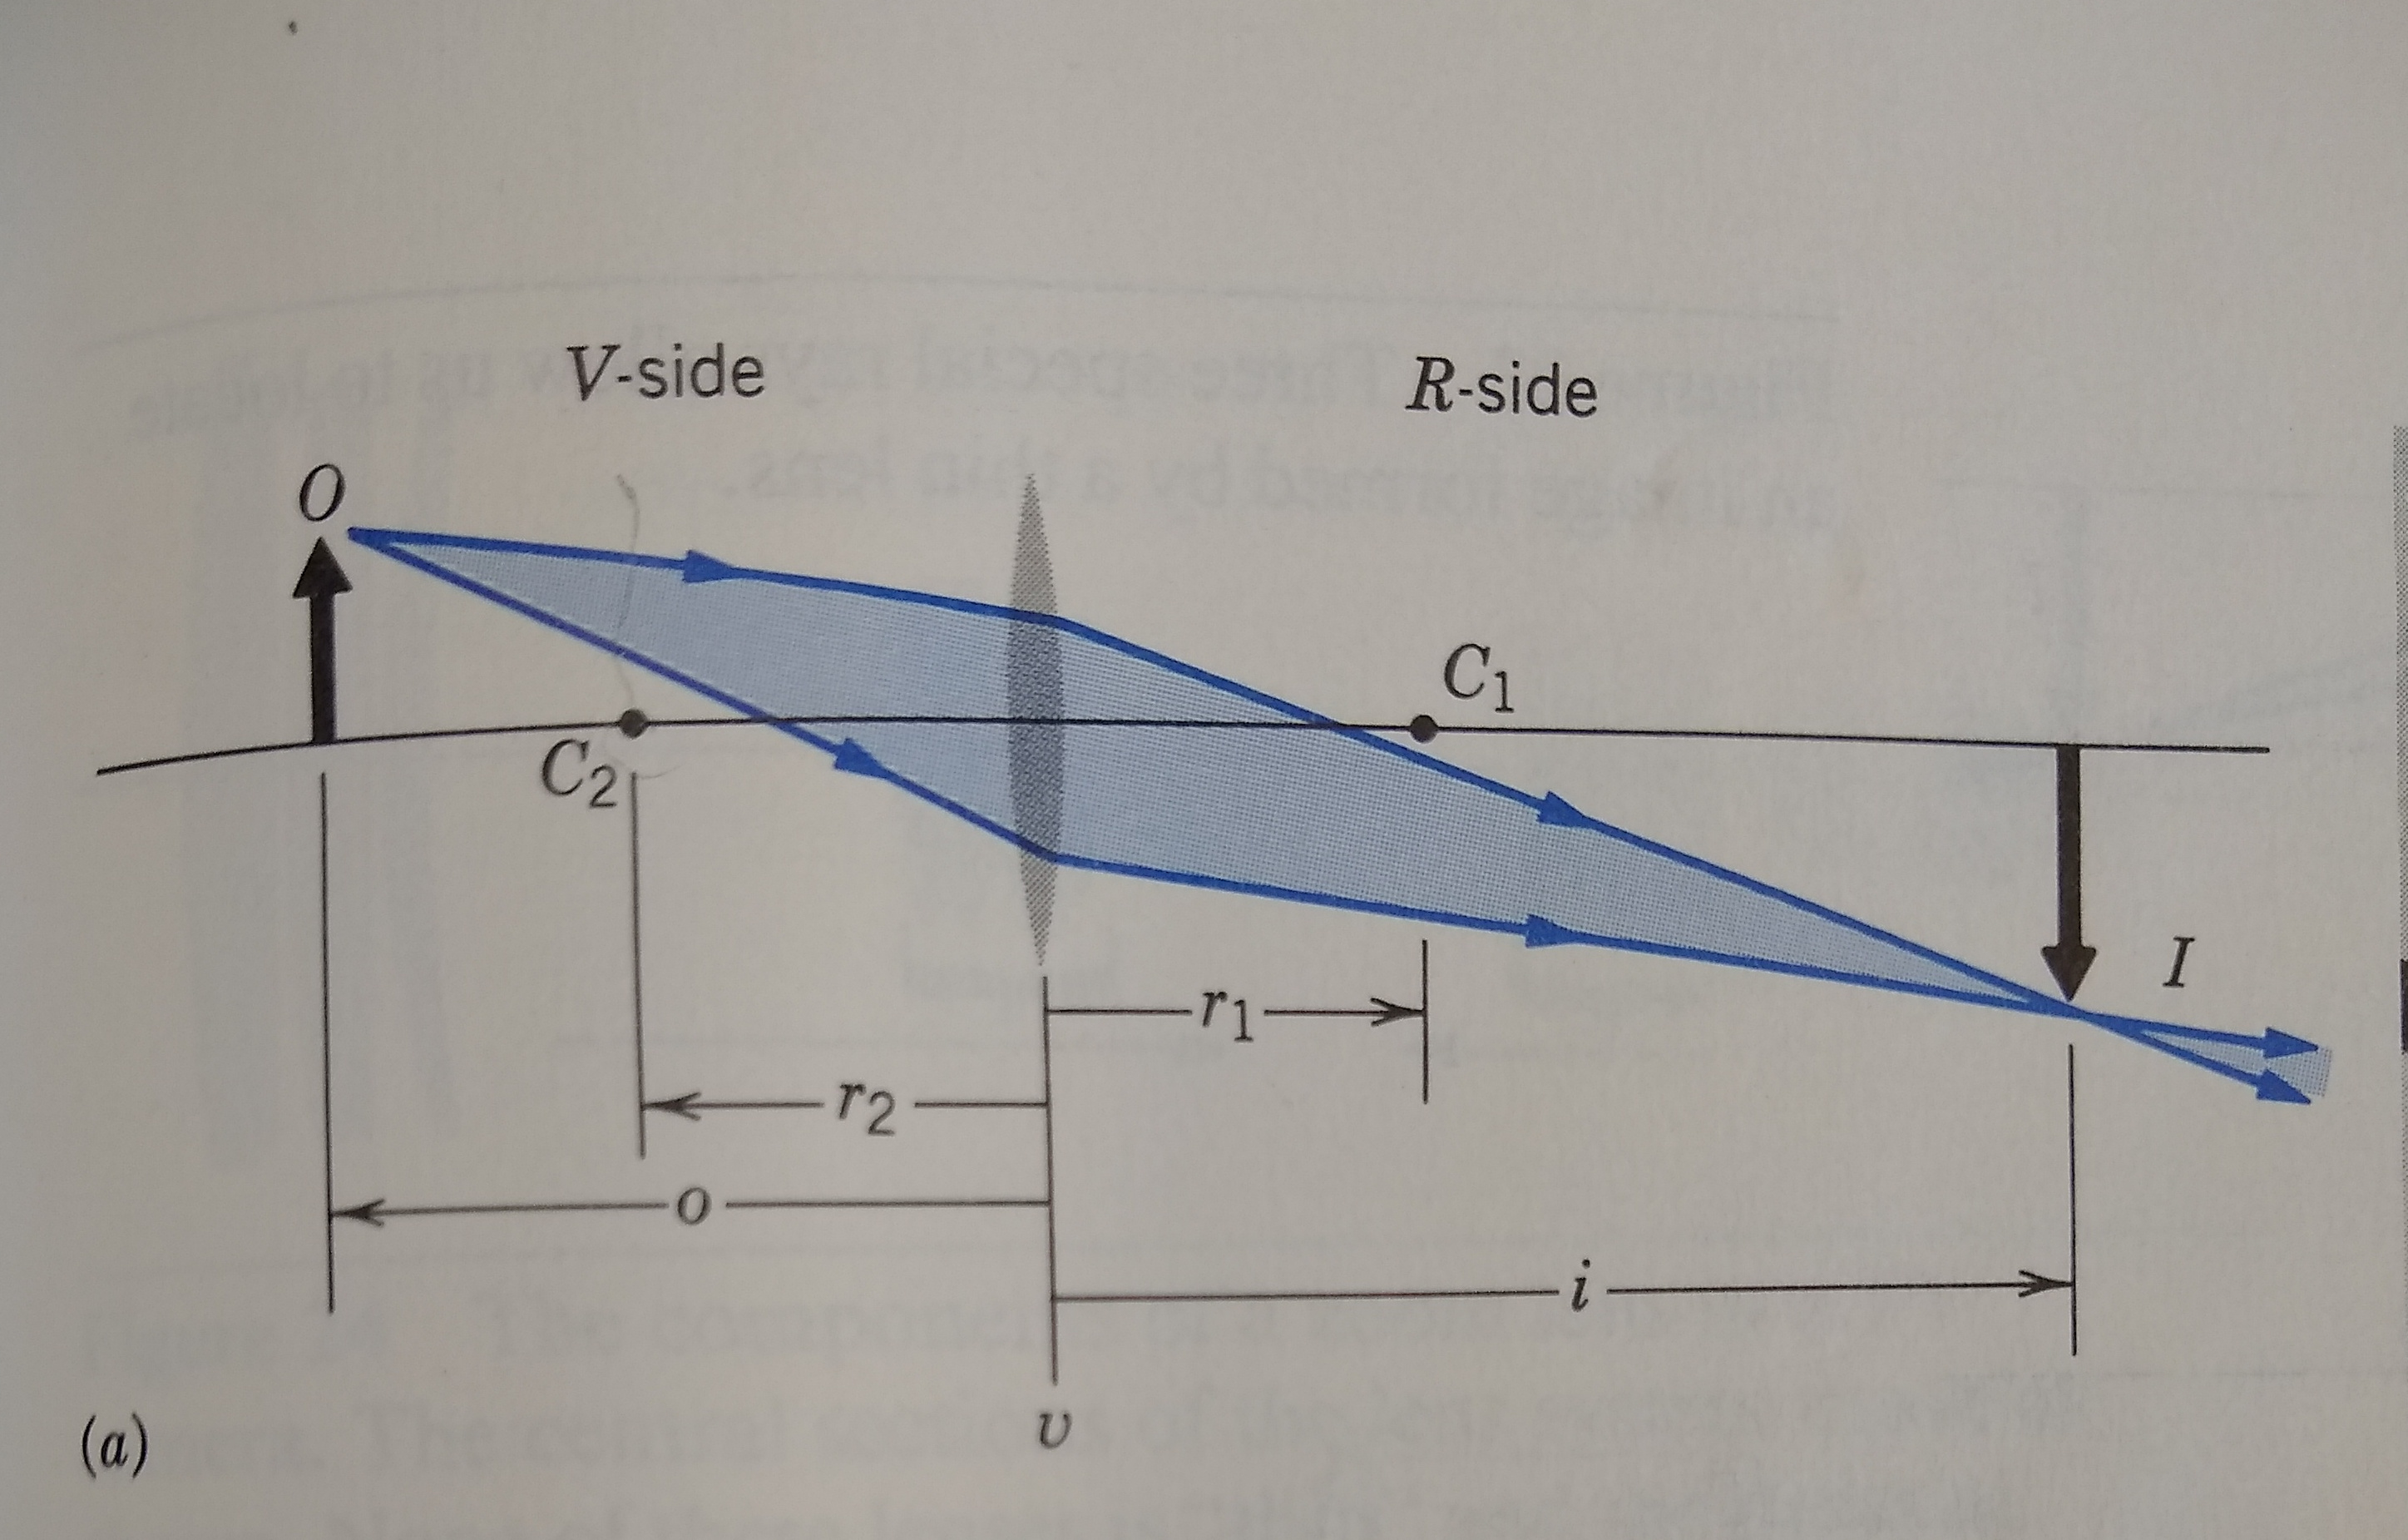
\includegraphics[width=\textwidth]{optics-halliday-resnick-crop.jpg}
                \newline
                
\includegraphics[width=\textwidth]{lens_geometry_invert.pdf}
            \end{center}

            
        \end{column}
    \end{columns}


}

\frame
{
    \begin{center}
        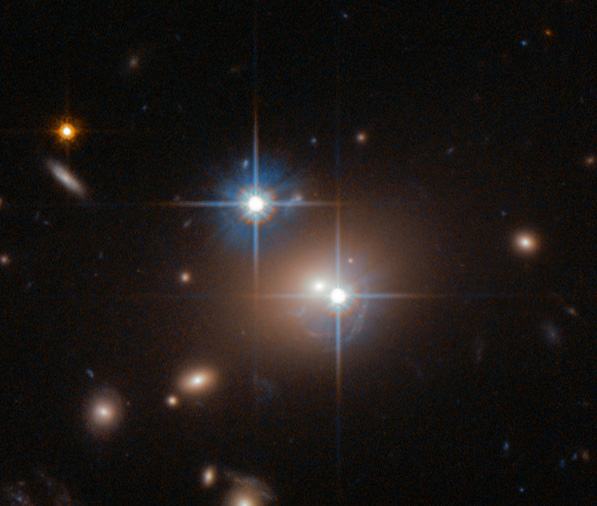
\includegraphics[width=0.4\textwidth]{QSO_B0957+0561-crop.jpg}
    \end{center}
    {\normalsize First Known Gravitational Lens: Two images of the same 
    object} {\tiny (QSO 0957+0561, image HST/NASA)}
}


\frame
{

    \frametitle{Using Gravitational Lensing}

    \setbeamerfont*{itemize/enumerate body}{size=\small}

    \begin{columns}
        \begin{column}{0.5\textwidth}
            \begin{itemize}

                \item The effect depends on the mass of the lens: we can measure the
                    mass of the lensing object!

                \item Lensing is especially useful for measuring dark matter.  The lensing
                    effect is present even if we can't see the mass.

            \end{itemize}
        \end{column}
        \begin{column}{0.5\textwidth}
            \begin{center}
                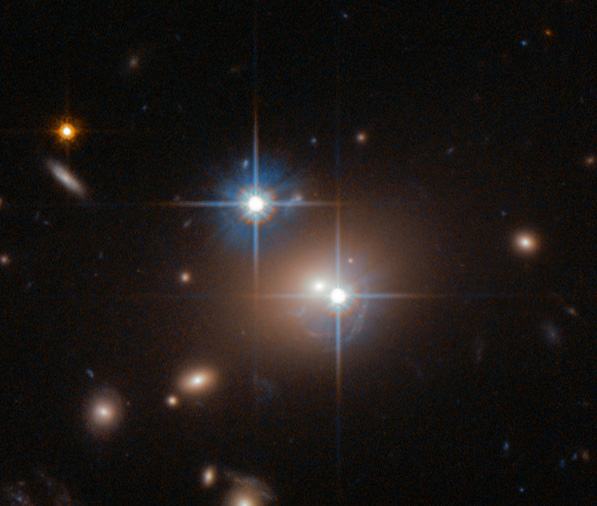
\includegraphics[width=0.7\textwidth]{QSO_B0957+0561-crop.jpg}
                \newline
                
\includegraphics[width=\textwidth]{lens_geometry_invert.pdf}
            \end{center}

            
        \end{column}
    \end{columns}


}

\frame
{

    \frametitle{Using Gravitational Lensing}

    \setbeamerfont*{itemize/enumerate body}{size=\small}

    \begin{columns}
        \begin{column}{0.5\textwidth}
            \begin{itemize}

                \item The effect depends on distances from observer to lens
                    and between lens and source.

                \item We can use lensing to infer distances.

                \item Farther distance means farther back in time, so we can
                    probe the expansion history of the universe and measure
                    the effects of Dark Energy

            \end{itemize}
        \end{column}
        \begin{column}{0.5\textwidth}
            \begin{center}
                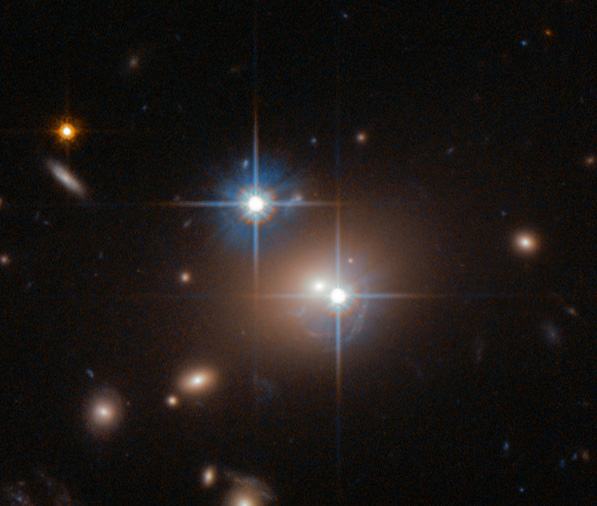
\includegraphics[width=0.7\textwidth]{QSO_B0957+0561-crop.jpg}
                \newline
                
\includegraphics[width=\textwidth]{lens_geometry_invert.pdf}
            \end{center}

            
        \end{column}
    \end{columns}


}

\frame
{

    \frametitle{Using Gravitational Lensing}

    \setbeamerfont*{itemize/enumerate body}{size=\small}

    \begin{columns}
        \begin{column}{0.5\textwidth}
            \begin{itemize}

                \item In practice lensing is basically sensitive to distance
                    {\em ratios}, but that's useful as well.

                \item This shows how strong the lensing effect is for
                    sources at different distances behind the lens

            \end{itemize}
        \end{column}
        \begin{column}{0.5\textwidth}
            \begin{center}
                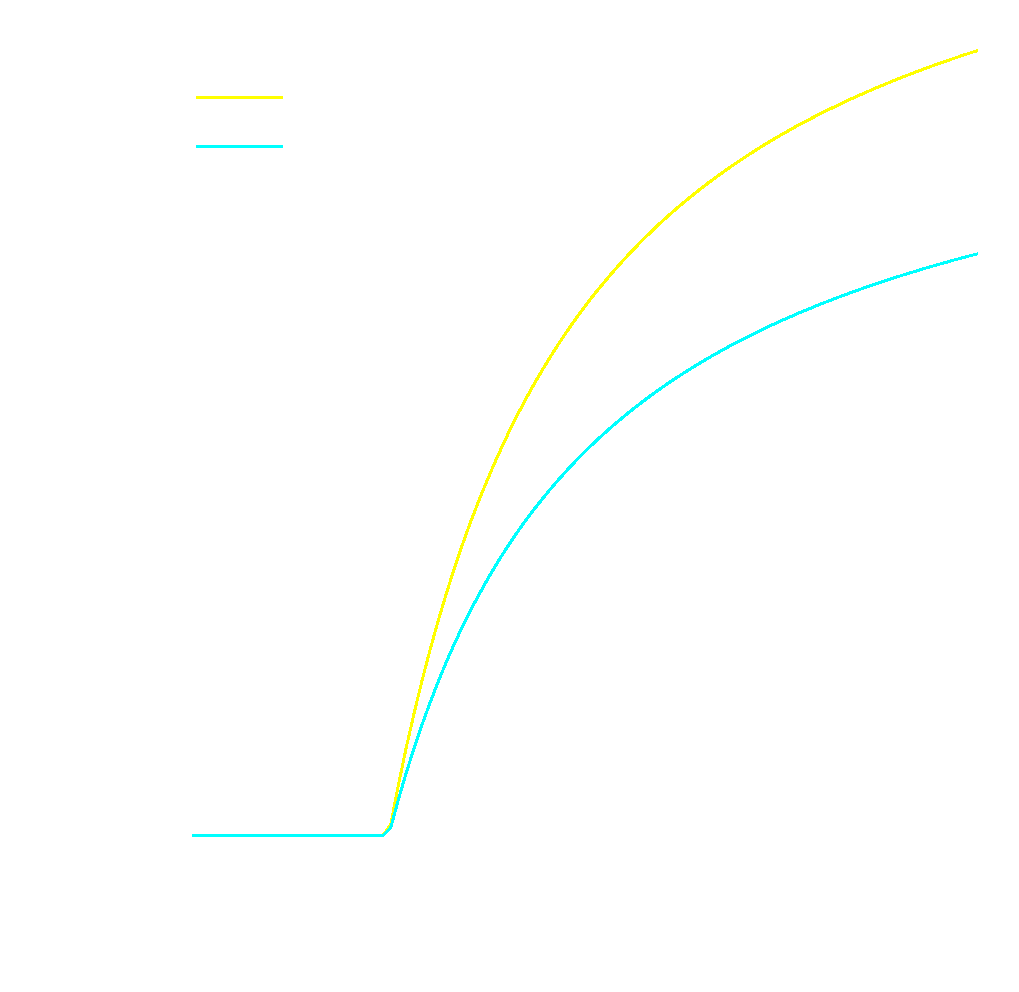
\includegraphics[width=\textwidth]{scinv-example-invert.pdf}
            \end{center}

            
        \end{column}
    \end{columns}


}




\frame
{

    \frametitle{Practical Lensing Measurements}

    \setbeamerfont*{itemize/enumerate body}{size=\small}

    \begin{columns}
        \begin{column}{0.5\textwidth}
            \begin{itemize}

                \item These examples I've shown are extremely rare. Not that useful
                    in general.

                \item But all objects in the universe are lensed by something.
                    The effect is just small.

                \item We can use this pervasive ``weak lensing'' effect to measure
                    the distribution of mass throughout the universe.

            \end{itemize}
        \end{column}
        \begin{column}{0.5\textwidth}
            \begin{center}
                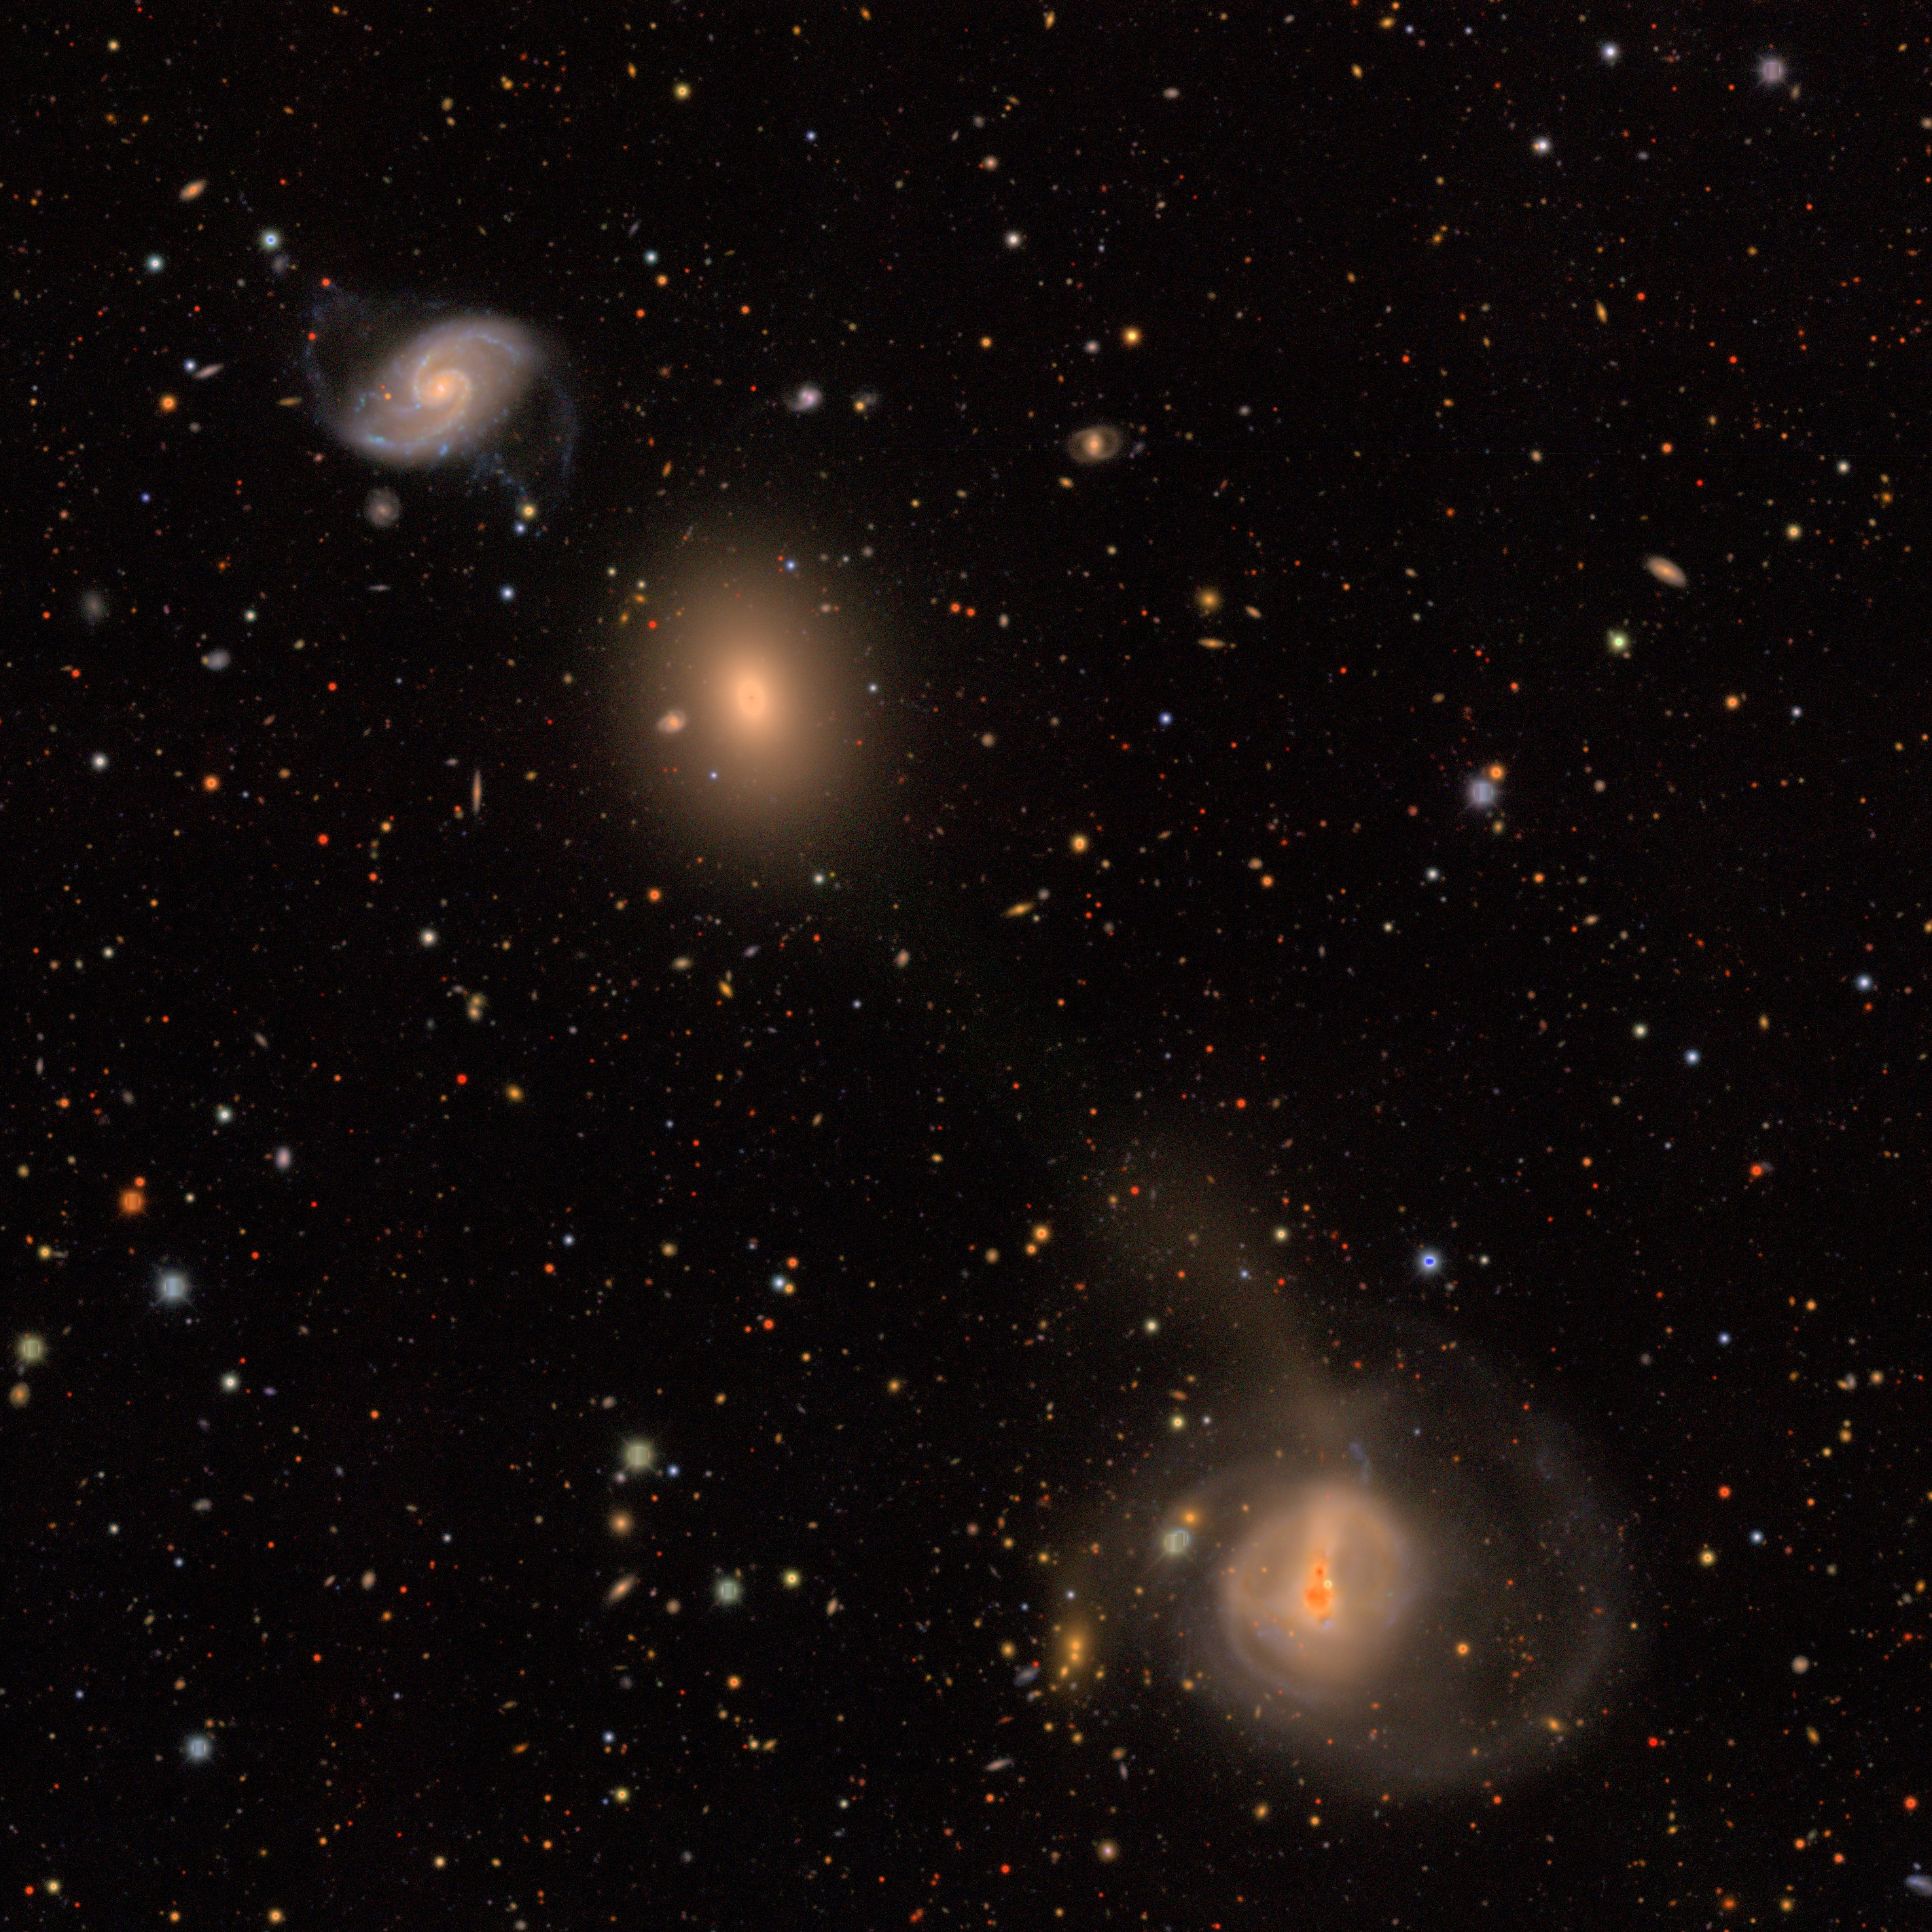
\includegraphics[width=\textwidth]{DES0428-4748-gri-crop.jpg}
                \newline
                {\tiny Dark Energy Survey, color image E. Sheldon}
            \end{center}

            
        \end{column}
    \end{columns}
}


\frame
{

    \frametitle{Weak Lensing}

    \setbeamerfont*{itemize/enumerate body}{size=\small}

    \begin{columns}
        \begin{column}{0.5\textwidth}
            \begin{itemize}

                \item A ray of light always looks like it came from a
                    larger angle offset from the lens.
                    
                \item But we don't know the original location, so that
                    displacement isn't generally useful.

                \item However, rays are generally displaced radially, so the
                    images of background galaxies get stretched a bit.
                    
                \item This stretching we can measure, because it is coherent:  all
                    the galaxies get stretched tangentially around the lens, making
                    a pattern.

            \end{itemize}
        \end{column}
        \begin{column}{0.5\textwidth}
            \begin{center}
                
\includegraphics[width=0.8\textwidth]{lens_geometry_invert.pdf}
                \newline
                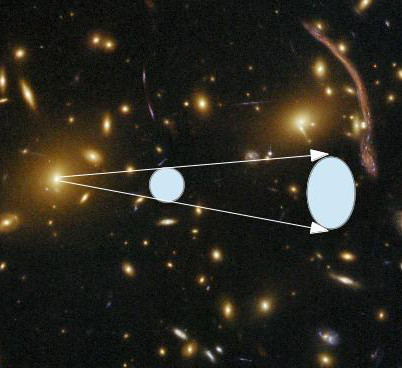
\includegraphics[width=0.7\textwidth]{shear-illustration-crop2.jpg}
            \end{center}

            
        \end{column}
    \end{columns}
}

\frame
{

    \frametitle{Weak Lensing}

    \setbeamerfont*{itemize/enumerate body}{size=\small}

    \begin{columns}
        \begin{column}{0.5\textwidth}
            \begin{itemize}

                \item We can measure the stretching pattern of galaxies.                   

                \item But the effect is {\em super} weak.  And galaxies are
                    not round anyway, which is like extra noise on the measurement.

                \item  We need to measure the ellipticities of millions of galaxies
                    and look for {\em correlations} in their ellipticities.

            \end{itemize}
        \end{column}
        \begin{column}{0.5\textwidth}
            \begin{center}
                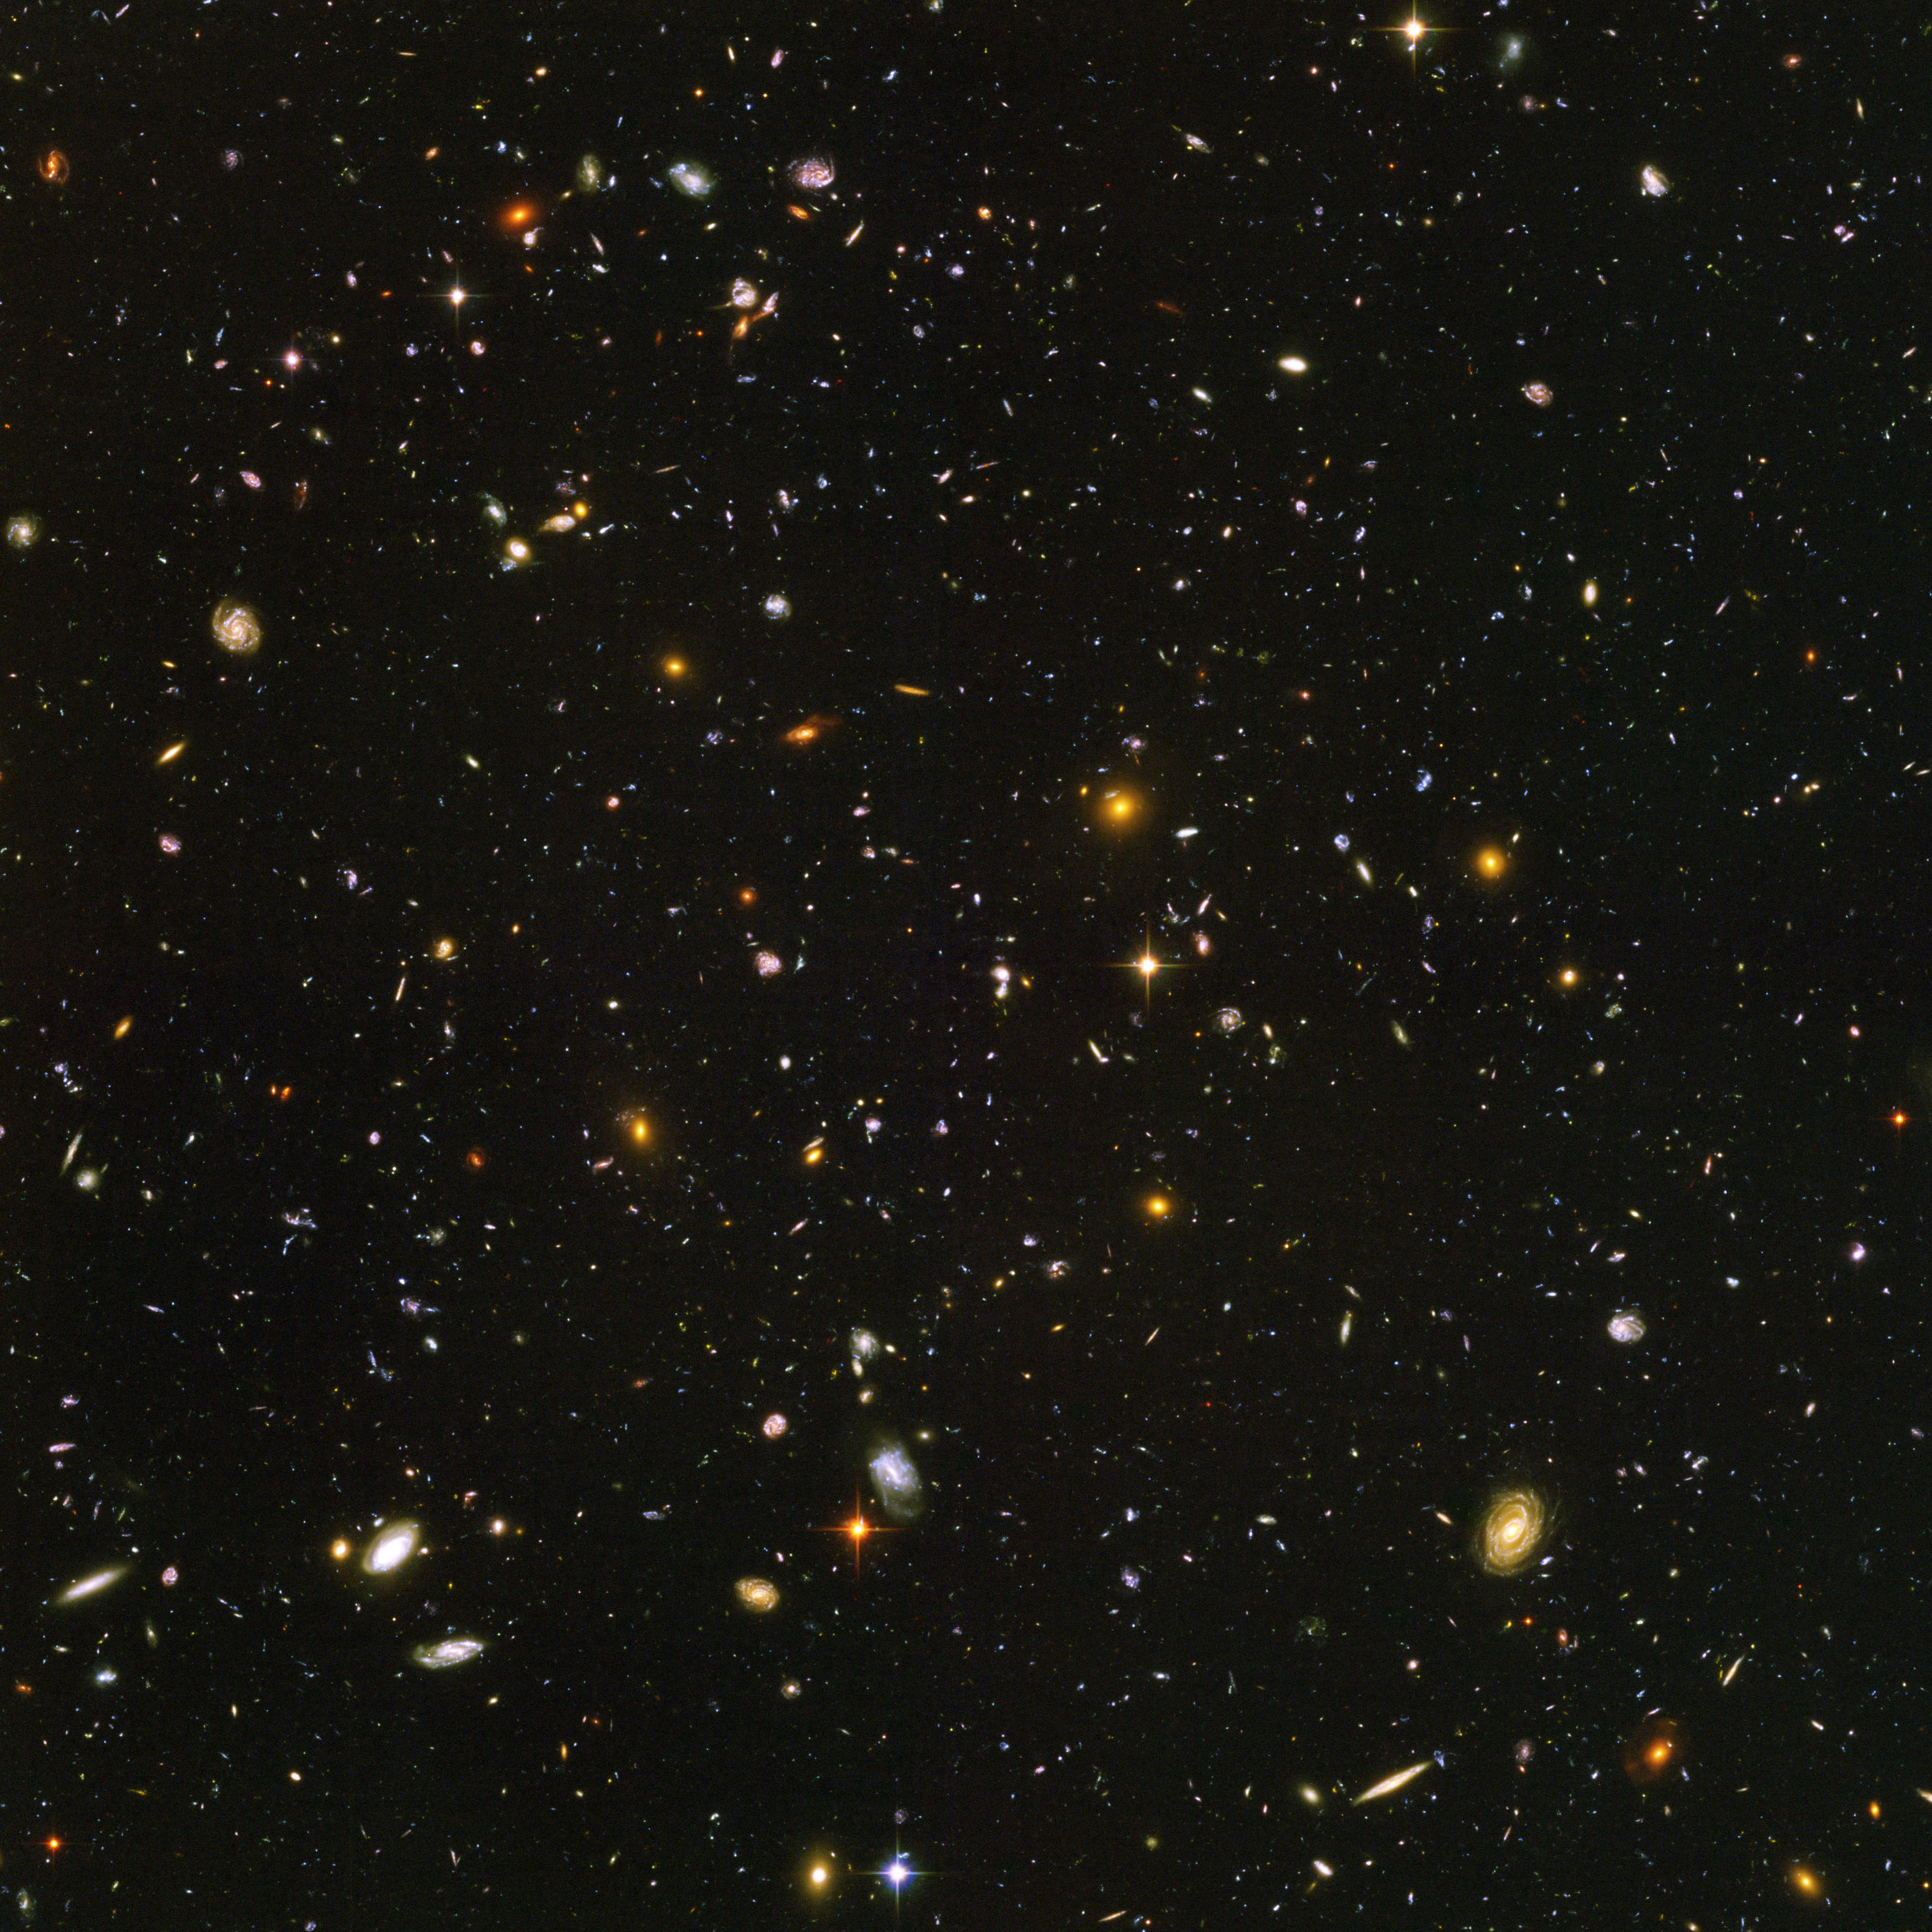
\includegraphics[width=\textwidth]{UDF_half.jpg}
            \end{center}

            
        \end{column}
    \end{columns}
}


\frame
{

    \frametitle{What Theory Predicts}

    \setbeamerfont*{itemize/enumerate body}{size=\large}

    \begin{itemize}

        \item The theory is gravity (general relativity) with dark matter, dark
            energy, and normal matter.

        \item The theory can predict (among other things):
            
            \begin{itemize}

                \item How the universe expands over time.

                \item How the light from distant galaxies is redshifted

                \item How the matter within the universe reacts to gravity, known
                    as ``clustering''.

            \end{itemize}

    \end{itemize}

}


\frame
{

    \frametitle{What Theory Predicts}


    \setbeamerfont*{itemize/enumerate body}{size=\large}

    \begin{itemize}

        \item How the universe is expanding

            \begin{itemize}
                    
                \item For two given galaxies, the distance between changes over
                    time {\color{gold} $|\Delta \vec{r} (t)|$ =
                     $| \vec{r}_1 - \vec{r}_2 |(t) $ }

                \item The relative velocity between galaxies is larger
                    for more separated galaxies

            \end{itemize}

        \item How the light from distant galaxies is redshifted {\color{gold}
            $z(|\Delta \vec{r}|)$}

        \item How the matter within the universe reacts to gravity over time.
            Gravity pulls matter together, and the density field
            in the universe evolves {\color{gold} $\rho(\vec{r},t)$}



    \end{itemize}

}

\frame
{

    \frametitle{Gravity Pulls Everything Together: Clustering}


    \setbeamerfont*{itemize/enumerate body}{size=\large}

    \begin{center}
        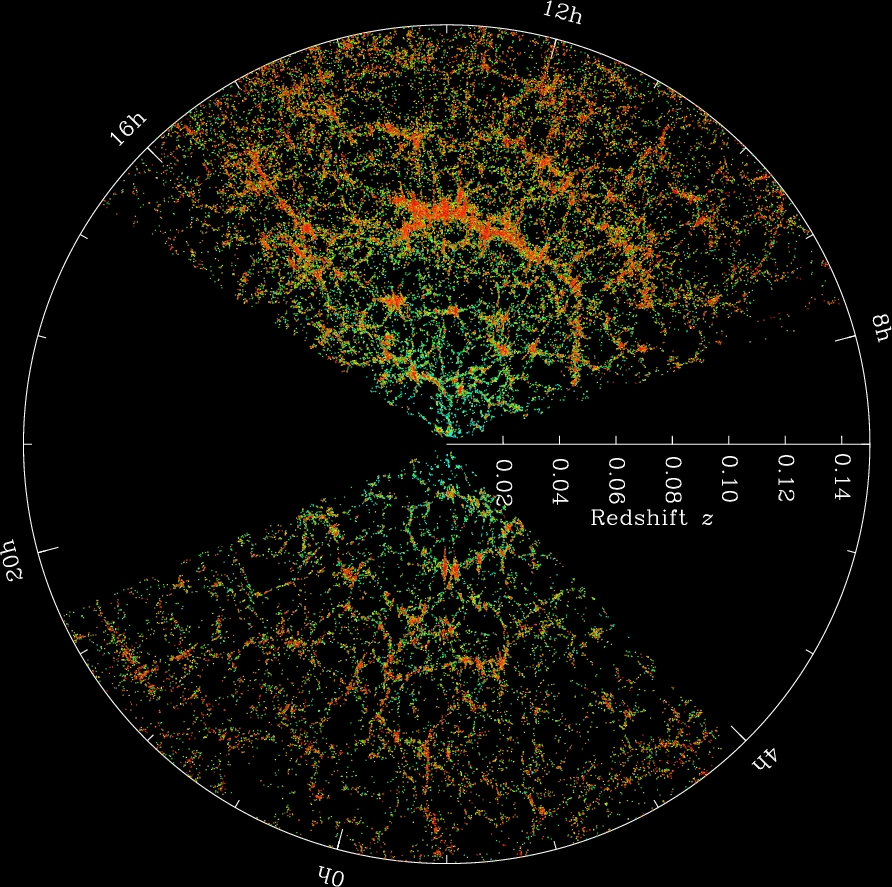
\includegraphics[width=0.5\textwidth]{orangepie.jpg}
    \end{center}

    Show Movie Mellenium Simulation

}


\frame
{

    \frametitle{What Theory Predicts}


    \begin{itemize}

            

        \item Expansion history: {\color{gold} $|\Delta \vec{r} (t)|$ }


        \item Redshift: {\color{gold} $z(|\Delta \vec{r}|)$}


        \item Density evolution: {\color{gold} $\rho(\vec{r},t)$}

        \item Recall from Paul's lecture: {\color{gold} $\Omega_m$} and
            {\color{gold} $\Omega_\Lambda$} were basic parameters in the
            Freedman Equations describing the expansion of the universe.


        \item Using these measurements we can learn about the mean mass density in
            the universe {\color{gold} $\Omega_m$}
            
        \item We can learn about the properties of dark energy, for example
            the density {\color{gold} $\Omega_\Lambda$}



    \end{itemize}

}

\frame
{

    \frametitle{Distance, Redshift and Density}

    \setbeamerfont*{itemize/enumerate body}{size=\large}

    \begin{itemize}

        \item The theory doesn't predict our particular universe

        \item The theory predicts {\em statistics} about these quantities
            
        \item Given the mean and variance of the mass density field, and the
            density of dark energy, it can predict

            \begin{itemize}

                \item {\color{gold} $\langle |\Delta \vec{r} (t)| \rangle$ }: Averaged
                    over a large number of objects

                \item {\color{gold} $\langle z(|\Delta \vec{r}|) \rangle$}

                \item {\color{gold} $\langle \rho(\vec{r_1}) \rho(\vec{r_2})
                    \rangle \propto \xi(|\vec{r_1} - \vec{r_2}|$) }: Correlation function

            \end{itemize}

    \end{itemize}

}


\frame
{

    \frametitle{Correlation Functions}

    \setbeamerfont*{itemize/enumerate body}{size=\small}

    \begin{columns}
        \begin{column}{0.5\textwidth}
            \begin{itemize}

                \item The theory predicts the correlation function of
                    dark matter 
                    {\color{gold} $\langle \rho(\vec{r_1}) \rho(\vec{r_2})
                    \rangle \propto \xi(|\vec{r_1} - \vec{r_2}|$) }

                \item For example, if a point in the universe has high density, a nearby
                    point probably also has high density. Similarly
                    for low density points.
                    
                \item So there should generally
                    be a positive correlation but it will decrease
                    for  points with larger separation.
                    
                \item The amplitude increases over time because gravity pulls
                    matter together, making it more spatially correlated


            \end{itemize}

        \end{column}
        \begin{column}{0.5\textwidth}
            \begin{center}
                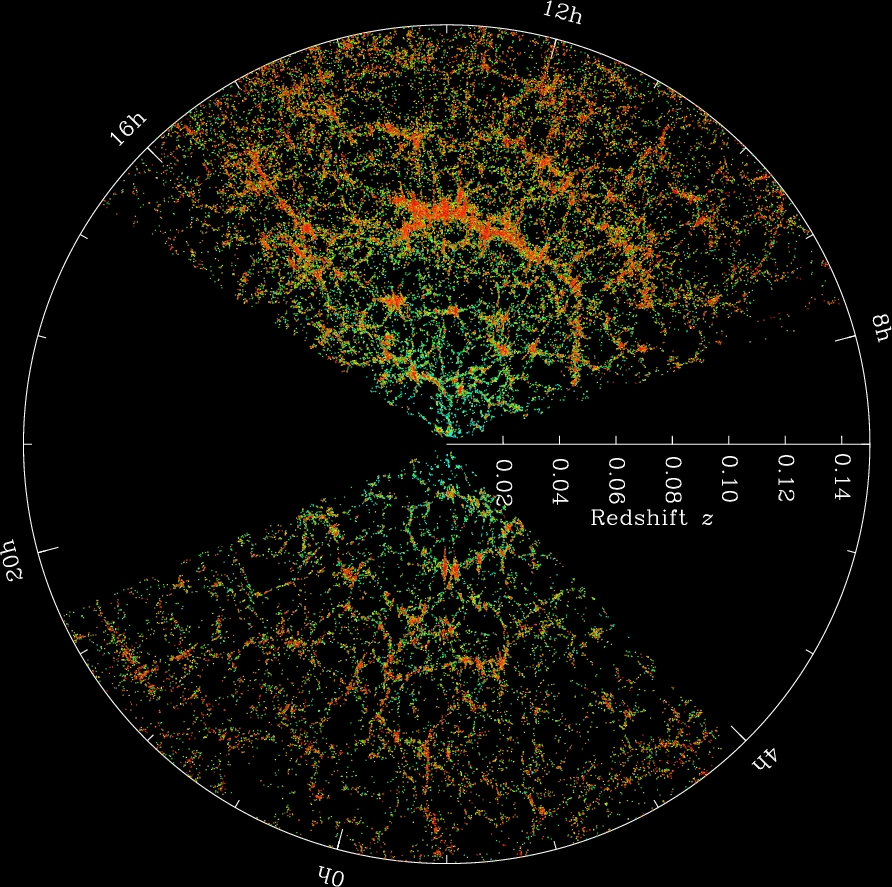
\includegraphics[width=\textwidth]{orangepie.jpg}
            \end{center}
            {\tiny SDSS Galaxy Locations (M. Blanton)}
        \end{column}

    \end{columns}


}

\frame
{

    \frametitle{Dark Matter Correlation Function}

    \setbeamerfont*{itemize/enumerate body}{size=\small}

    \begin{columns}
        \begin{column}{0.5\textwidth}
            \begin{itemize}

                \item The theory predicts the correlation function of
                    dark matter
                    {\color{gold} $\langle \rho(\vec{r_1}) \rho(\vec{r_2})
                    \rangle \propto \xi(|\vec{r_1} - \vec{r_2}|$) }

                \item Depends on the mean density and variance of the matter 
                    in the universe

                \item Evolution also depends on the dark energy
 
                \item Galaxies are only located at the highest density points,
                    not ideal.  But we can measure this better using
                    {\color{lightskyblue} gravitational lensing}

            \end{itemize}

        \end{column}
        \begin{column}{0.5\textwidth}
            \begin{center}
                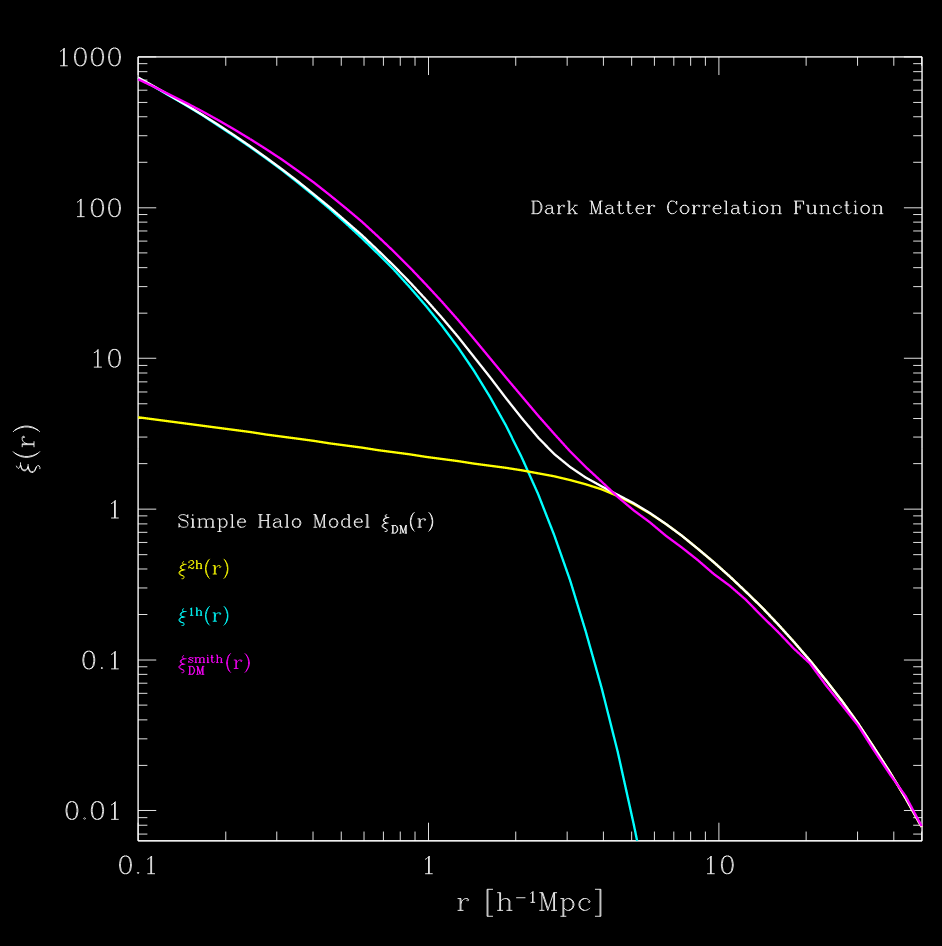
\includegraphics[width=\textwidth]{zentner-halo-model-inv.png}
            \end{center}
            {\tiny A. Zentner}
        \end{column}

    \end{columns}


}


\frame
{

    \frametitle{Dark Matter Correlation Function}

    \setbeamerfont*{itemize/enumerate body}{size=\footnotesize}

    \begin{columns}
        \begin{column}{0.5\textwidth}
            \begin{itemize}

                \item The lensing from foreground masses
                    causes correlations in the ellipticities of background
                    galaxies

                \item We can measure the correlation function in the
                    ellipticity {\color{gold} $\langle e(\vec{\theta_1})
                    e(\vec{\theta_2}) \rangle$ }

                \item Because the correlations in the ellipticities are caused
                    by mass, this is closely related to the correlation
                    function of the mass, which is what the theory predicts
                    {\color{gold} $\langle \rho(\vec{r_1}) \rho(\vec{r_2})
                    \rangle$ }

            \end{itemize}

        \end{column}
        \begin{column}{0.5\textwidth}
            \begin{center}
                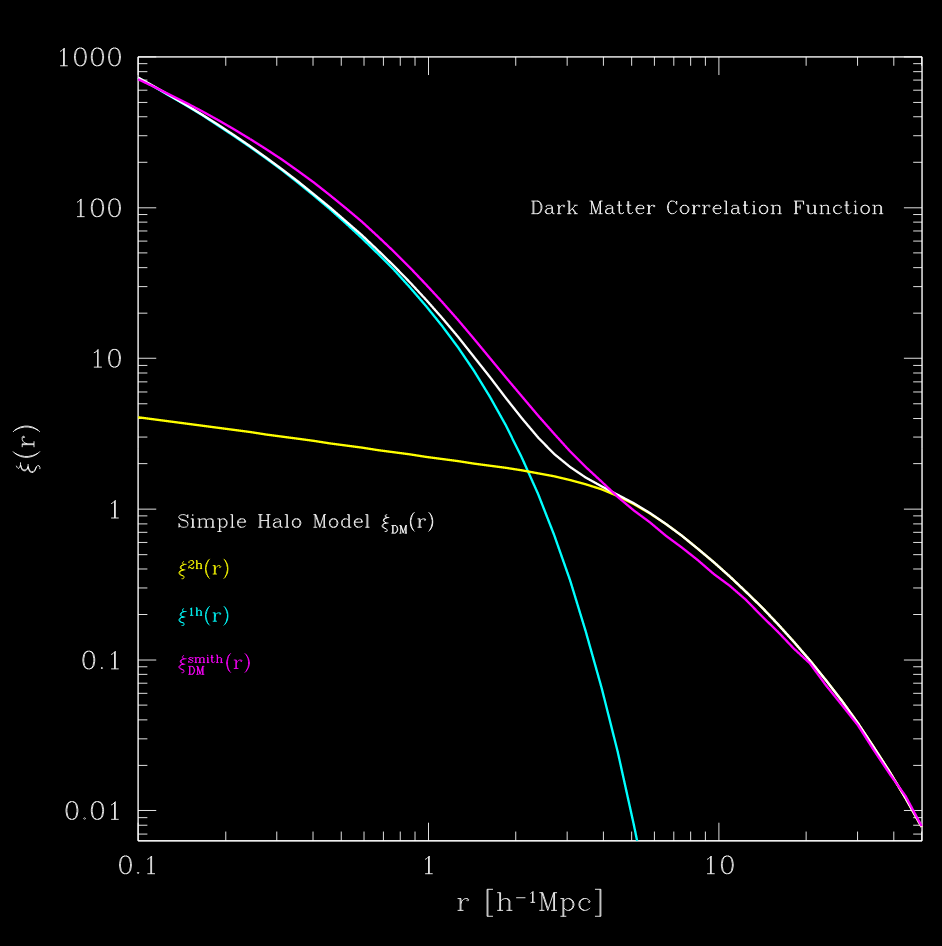
\includegraphics[width=\textwidth]{zentner-halo-model-inv.png}
            \end{center}
            {\tiny A. Zentner}
        \end{column}

    \end{columns}


}

\frame
{

    \frametitle{Dark Matter Correlation Function}

    \setbeamerfont*{itemize/enumerate body}{size=\footnotesize}

    \begin{columns}
        \begin{column}{0.5\textwidth}
            \begin{itemize}

                \item We can do a special measurement where we look
                    specifically around foreground objects, rather
                    than just correlating all shapes

                \item Then we measure the mean amount of mass in the lens, for
                    example galaxies.

                \item Can we measure the dark matter in galaxies?

            \end{itemize}

        \end{column}
        \begin{column}{0.5\textwidth}
            \begin{center}
                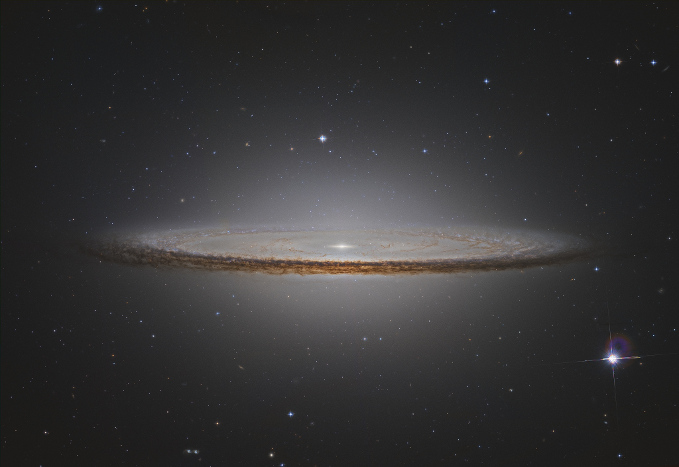
\includegraphics[width=0.8\textwidth]{M104b_peris2048_scale_small.jpg}
                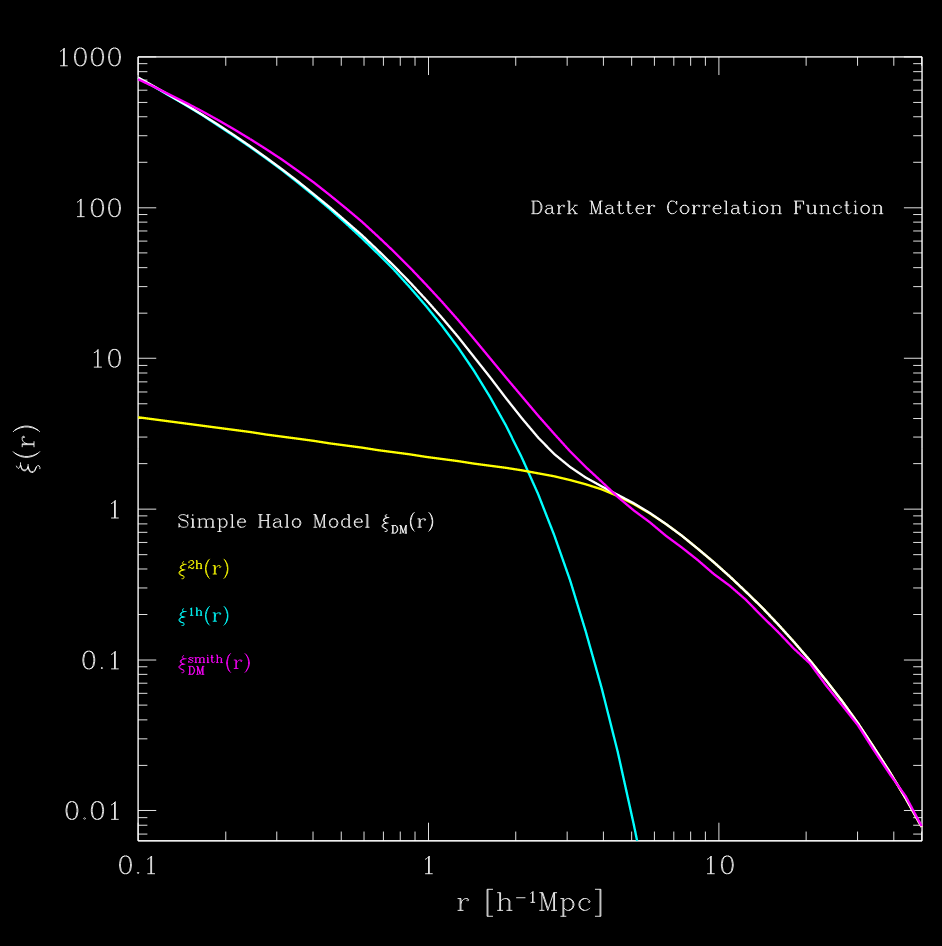
\includegraphics[width=0.8\textwidth]{zentner-halo-model-inv.png}
            \end{center}
        \end{column}

    \end{columns}


}

\frame
{

    \frametitle{Using Gravitational Lensing}

    \setbeamerfont*{itemize/enumerate body}{size=\small}

    \begin{columns}
        \begin{column}{0.5\textwidth}
            \begin{itemize}

                \item Plus, with lensing we can re-measure the signal for
                    objects at different {\em redshifts} learn about their {\em
                    distances} from us.

                \item This is especially useful for studying Dark Energy

            \end{itemize}
        \end{column}
        \begin{column}{0.5\textwidth}
            \begin{center}
                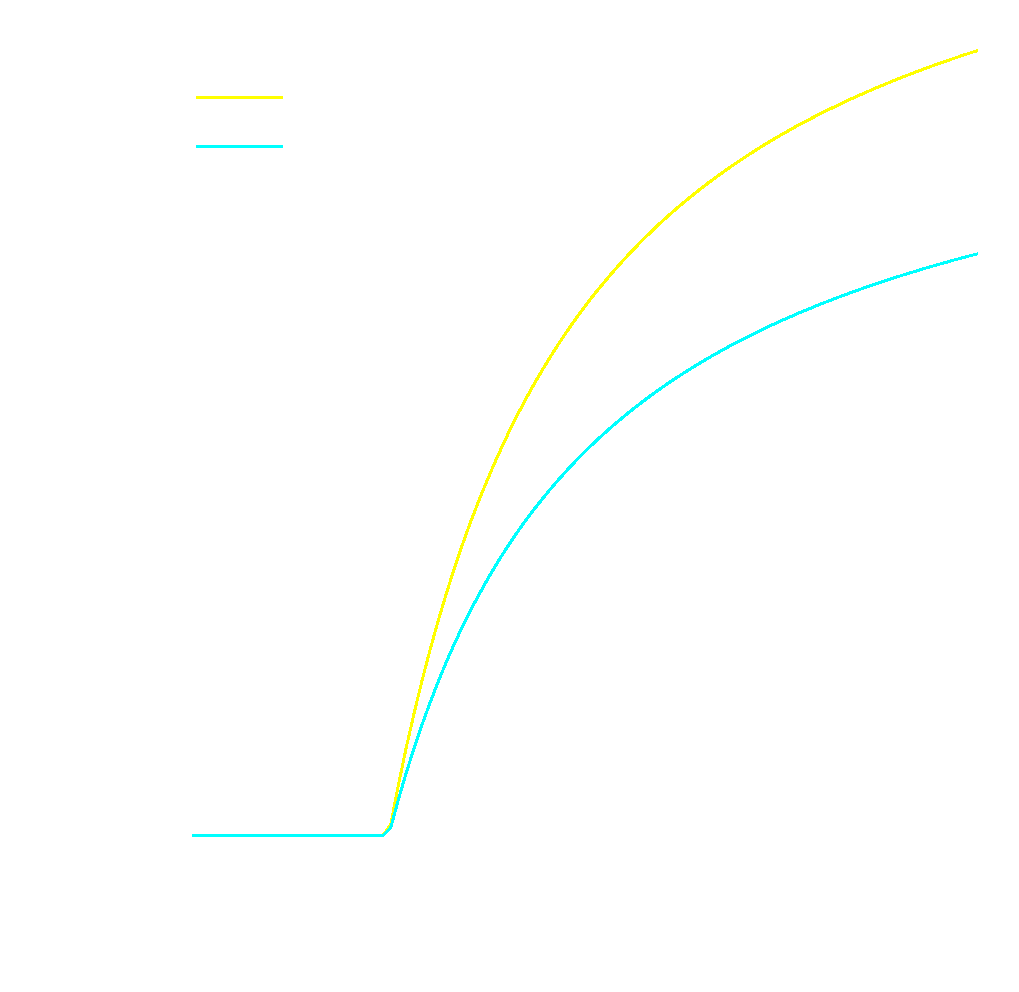
\includegraphics[width=\textwidth]{scinv-example-invert.pdf}
            \end{center}

            
        \end{column}
    \end{columns}


}

\frame
{

    \frametitle{Dark Energy Survey}

    \setbeamerfont*{itemize/enumerate body}{size=\small}

    \begin{columns}
        \begin{column}{0.5\textwidth}
            \begin{itemize}

                \item We perform weak lensing measurements using data we take
                    with the Blanco telescope in Chile

                \item We built a new camera specifically to do weak lensing and
                    study Dark Energy

            \end{itemize}

        \end{column}
        \begin{column}{0.5\textwidth}
            \begin{center}
                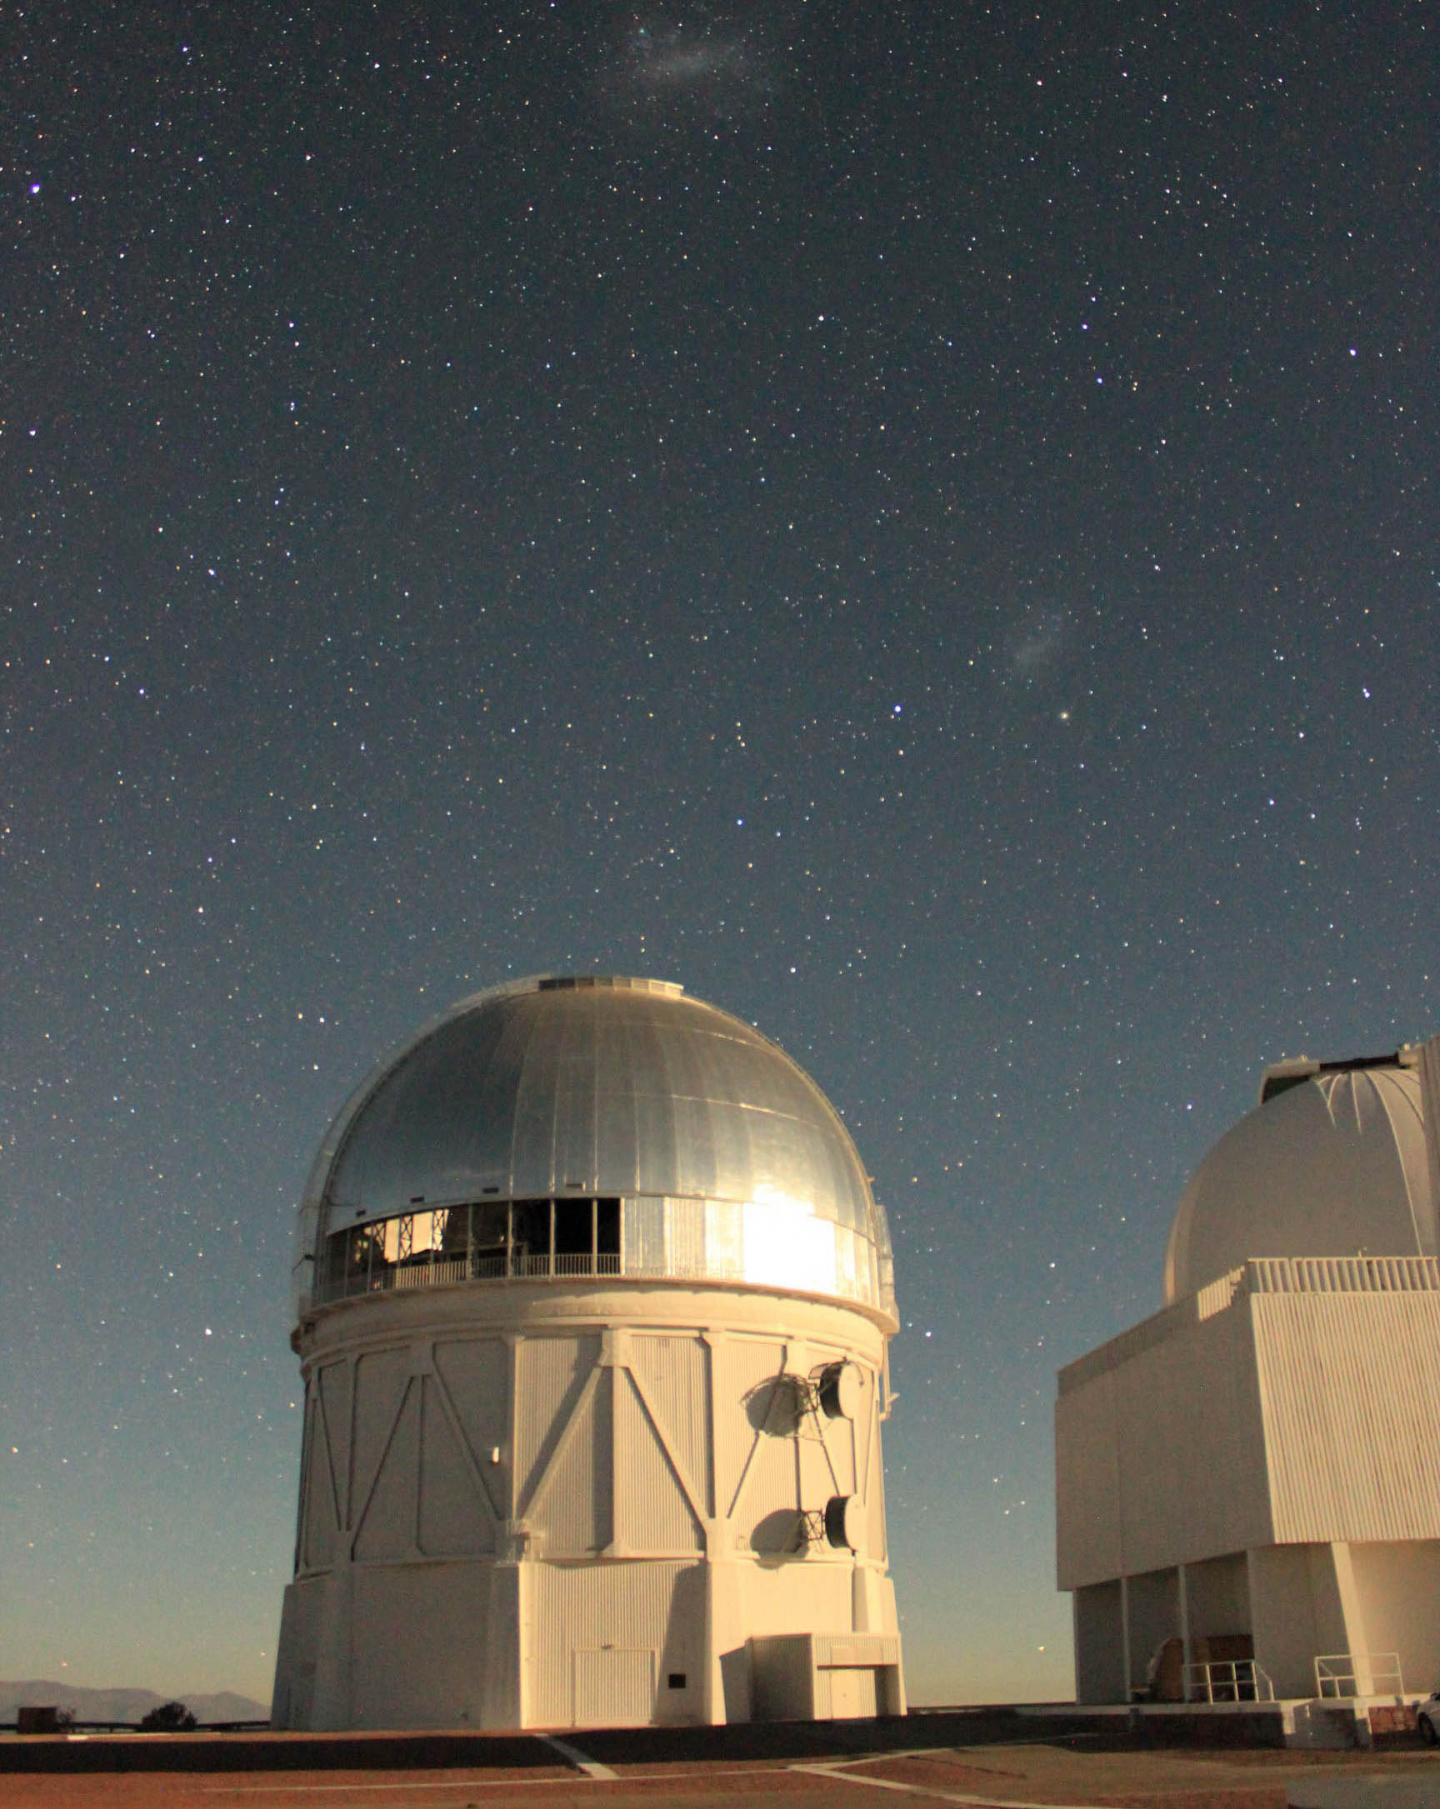
\includegraphics[height=0.7\textheight]{blanco-dustin-lang.jpg}
                \newline
                {\tiny Blanco Telescope in Chile (D. Lang)}
            \end{center}
        \end{column}

    \end{columns}


}



\frame
{

    \frametitle{Dark Energy Survey}

    \setbeamerfont*{itemize/enumerate body}{size=\small}

    \begin{columns}
        \begin{column}{0.5\textwidth}
            \begin{itemize}

                \item We perform weak lensing measurements using data we take
                    with the Blanco telescope in Chile

                \item We built a new camera specifically to do weak lensing and
                    study Dark Energy

            \end{itemize}

        \end{column}
        \begin{column}{0.5\textwidth}
            \begin{center}
                \includegraphics[height=0.7\textheight]{ctio_blanco_crew_2013Oct-30-small-balance.jpg}
                \newline
                {\tiny Blanco Telescope in Chile (B. Nord)}
            \end{center}
        \end{column}

    \end{columns}


}


\frame
{
    \begin{center}
        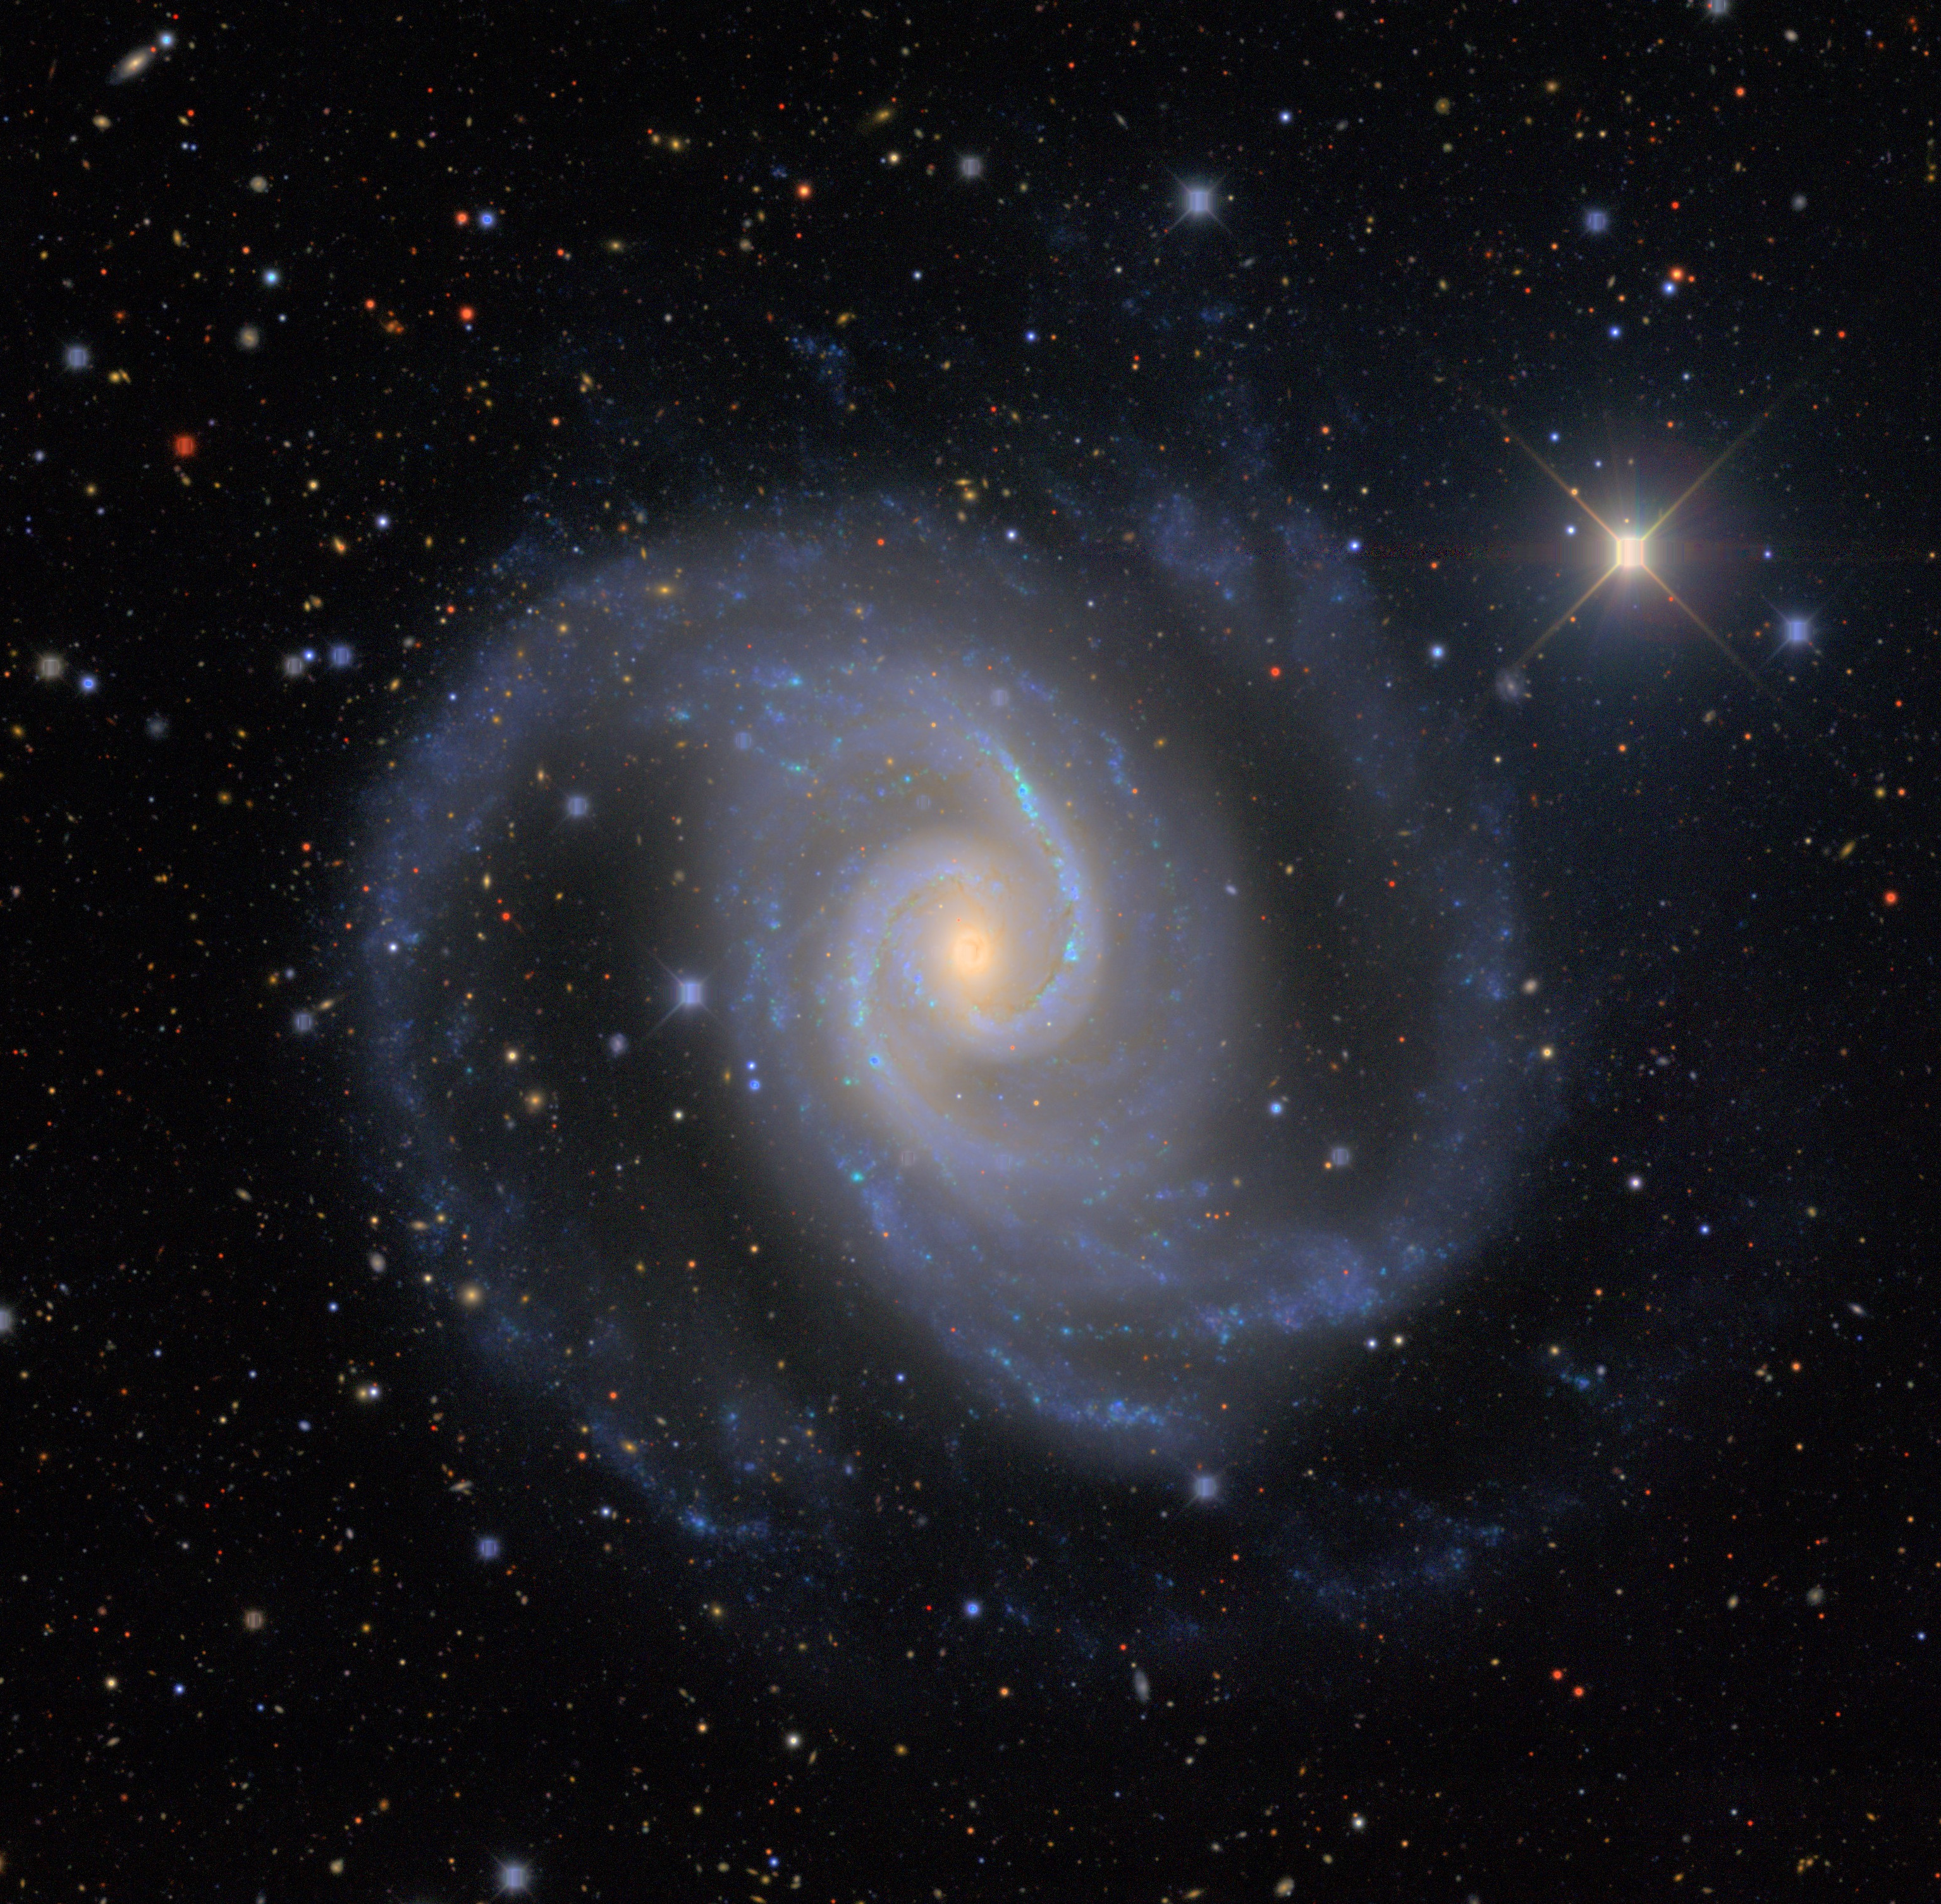
\includegraphics[width=0.8\textwidth]{DES0421-5457-gri-ngc1566.jpg}
    \end{center}
    {\normalsize Dark Energy Survey (E. Sheldon)}
}


\frame
{

    \frametitle{Dark Matter in Galaxies}

    \setbeamerfont*{itemize/enumerate body}{size=\small}

    \begin{columns}
        \begin{column}{0.5\textwidth}
            \begin{itemize}

                \item Measure the correlation of ellipticities with
                    positions of galaxies

                \item If all the light were in stars only, the curve would
                    be much steeper on small scales

                \item On large scales the signal is due to nearby objects, but
                    the amplitude is way too high if the mass were only from
                    stars

                \item In excellent agreement with prediction of cold dark
                    matter theory

            \end{itemize}

        \end{column}
        \begin{column}{0.5\textwidth}
            \begin{center}
                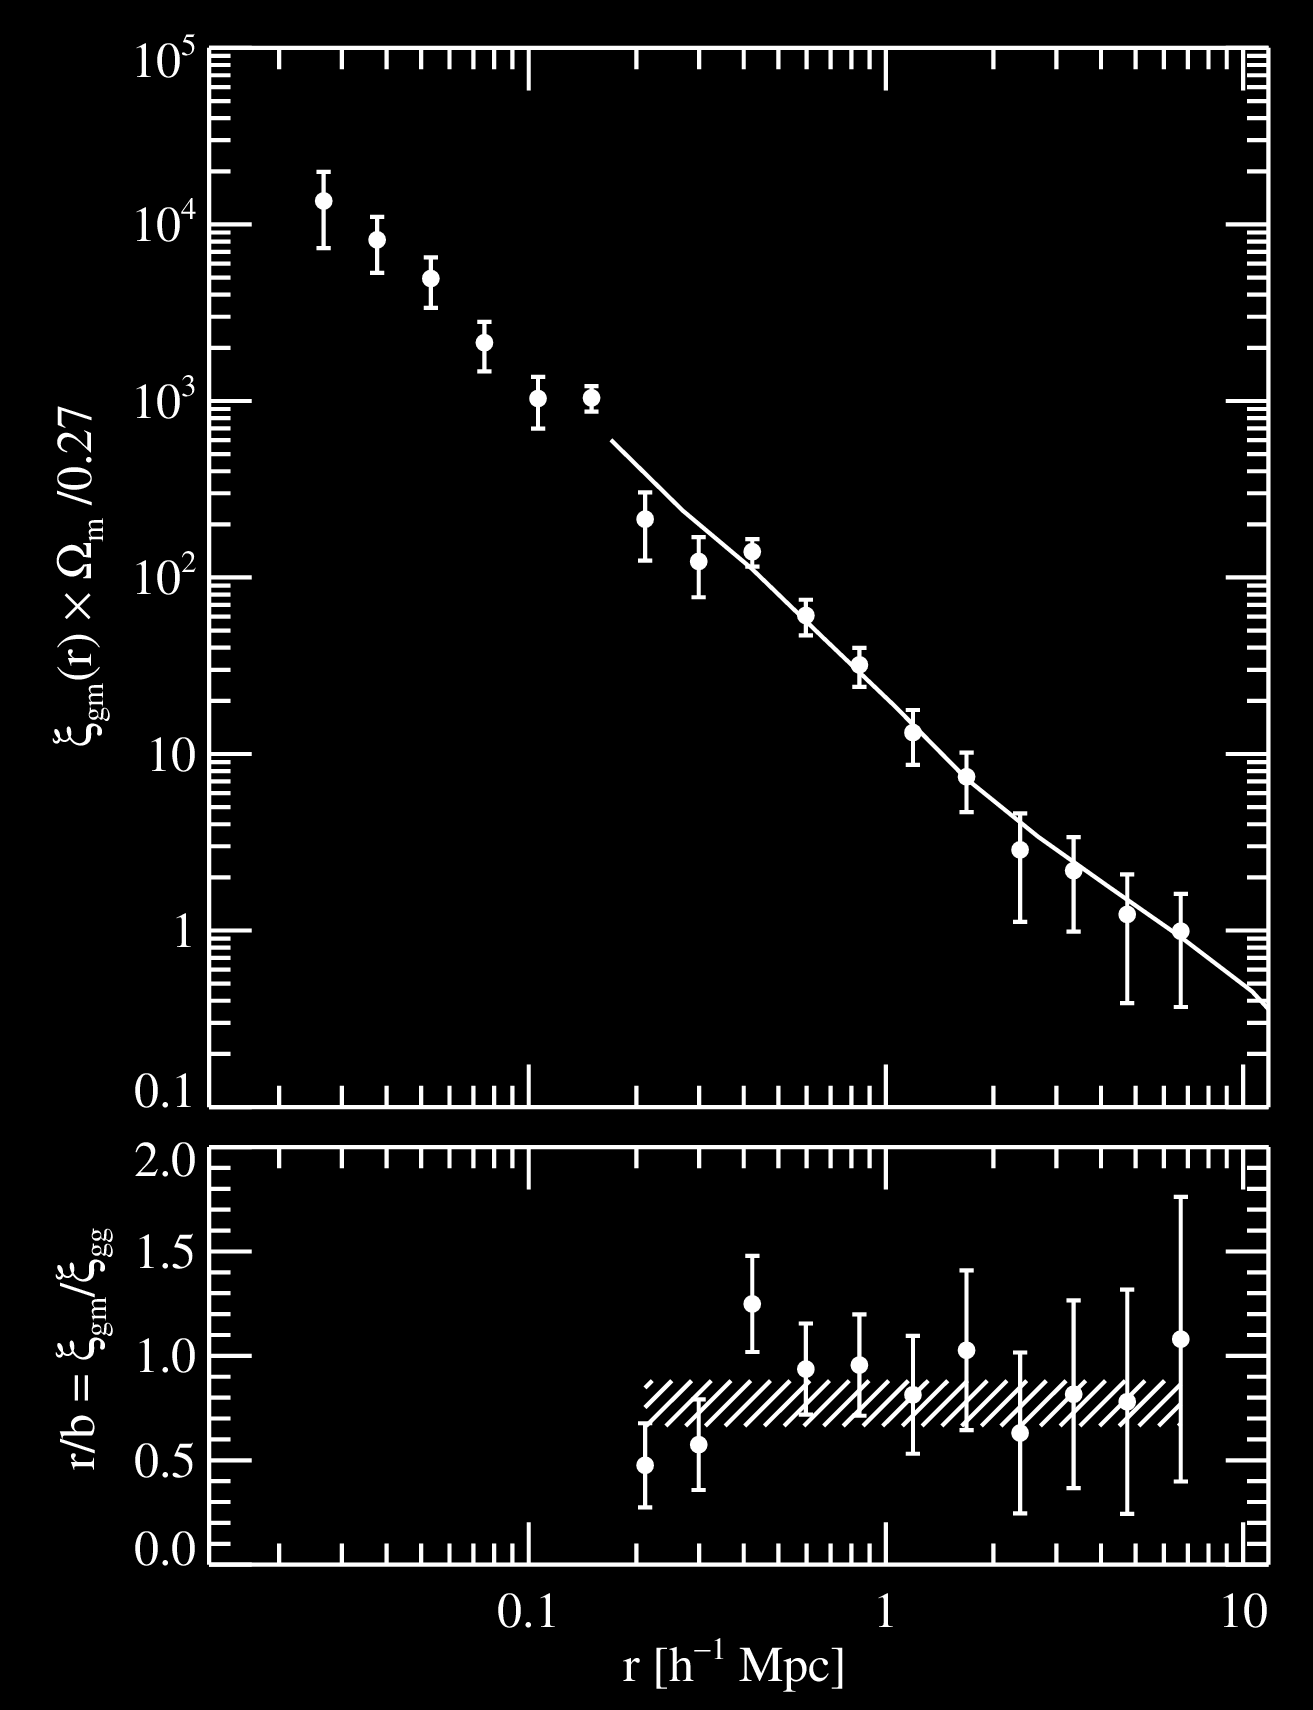
\includegraphics[width=\textwidth]{xi_all_idit_bias_icolor-crop.png}
                \newline
                {\tiny E. Sheldon}
            \end{center}
        \end{column}

    \end{columns}


}


\frame
{

    \frametitle{Weak Lensing Shear Correlation Function}

    \setbeamerfont*{itemize/enumerate body}{size=\small}

    \begin{columns}
        \begin{column}{0.5\textwidth}
            \begin{itemize}

                \item Now just correlate the shapes, don't look around
                    specific points {\color{gold} $\langle e(\vec{\theta_1})
                    e(\vec{\theta_2}) \rangle$ }

                \item Recall this is realted to the correlation function
                    of the density field
                    {\color{gold} $\langle \rho(\vec{r_1}) \rho(\vec{r_2})
                    \rangle \propto \xi(|\vec{r_1} - \vec{r_2}|$) }

            \end{itemize}

        \end{column}
        \begin{column}{0.5\textwidth}
            \begin{center}
                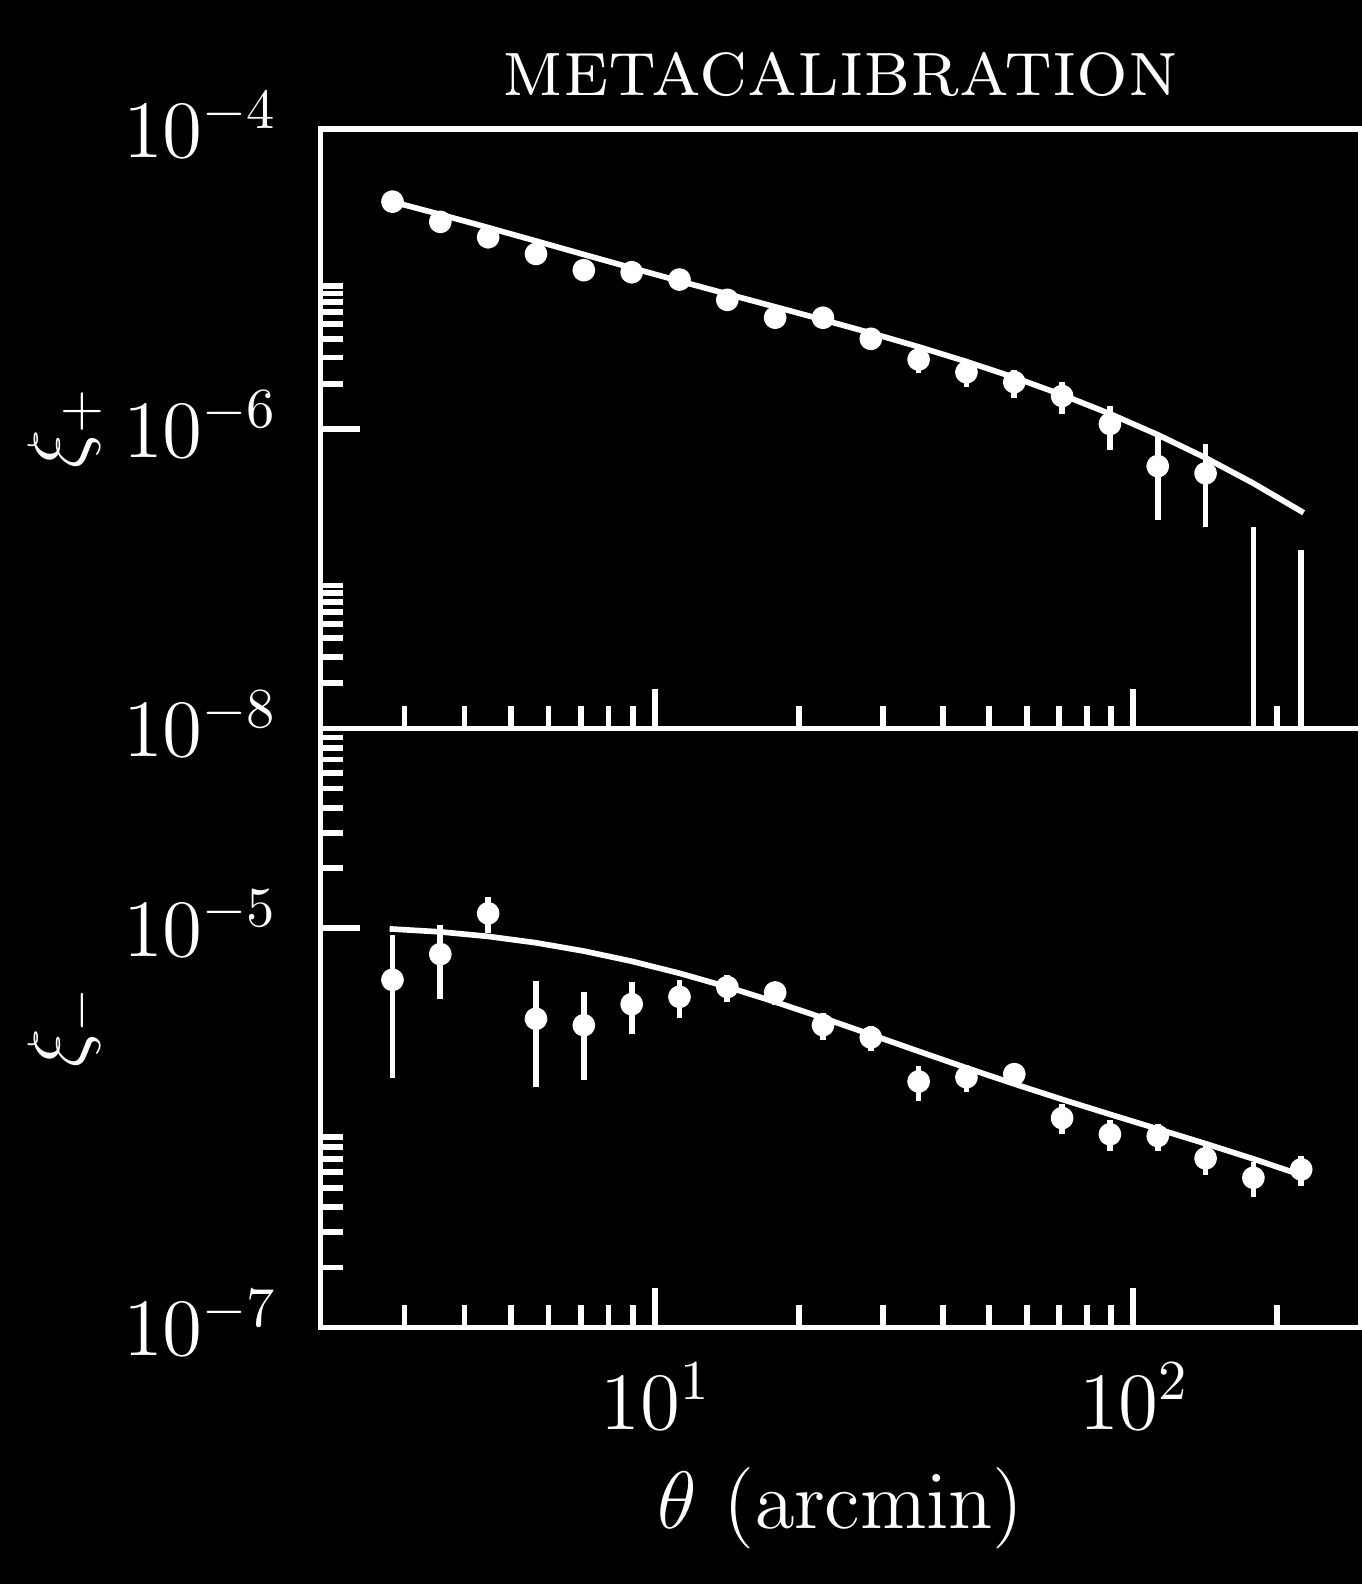
\includegraphics[width=\textwidth]{xi_notomo_neg.png}
                \newline
                {\tiny Dark Energy Survey}
            \end{center}
        \end{column}

    \end{columns}


}


\frame
{

    \frametitle{Weak Lensing Shear And Cosmology}

    \setbeamerfont*{itemize/enumerate body}{size=\small}

    \begin{columns}
        \begin{column}{0.5\textwidth}
            \begin{itemize}

                \item DES constrains {\color{gold} $\Omega_m$}, {\color{gold} $\Omega_\Lambda$}
                    and the mass variance very well.

                \item Agrees with the cosmic microwave background.
                    
                \item Combining the two is even better.

            \end{itemize}

        \end{column}
        \begin{column}{0.5\textwidth}
            \begin{center}
                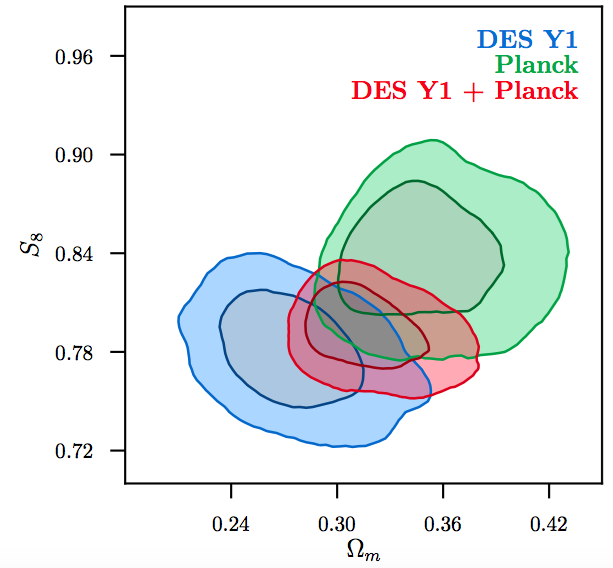
\includegraphics[width=\textwidth]{3x2-fig10.png}
                \newline
                {\tiny Dark Energy Survey}
            \end{center}
        \end{column}

    \end{columns}


}

\frame
{

    \frametitle{Weak Lensing Shear And Cosmology}

    \setbeamerfont*{itemize/enumerate body}{size=\small}

    \begin{columns}
        \begin{column}{0.5\textwidth}
            \begin{itemize}

                \item What about Dark Energy?

                \item If it is vacuum energy, we expect the density to
                    be simply related to the pressure: {\color{gold} $p = -\rho$}.

                \item To test if it is different, we can try
                    to measure {\color{gold} $p = w \rho$}, then measure {\color{gold} $w$}.

                \item So far it looks close to {\color{gold} $w = -1$}. Mostly informed
                    by other data.

            \end{itemize}

        \end{column}
        \begin{column}{0.5\textwidth}
            \begin{center}
                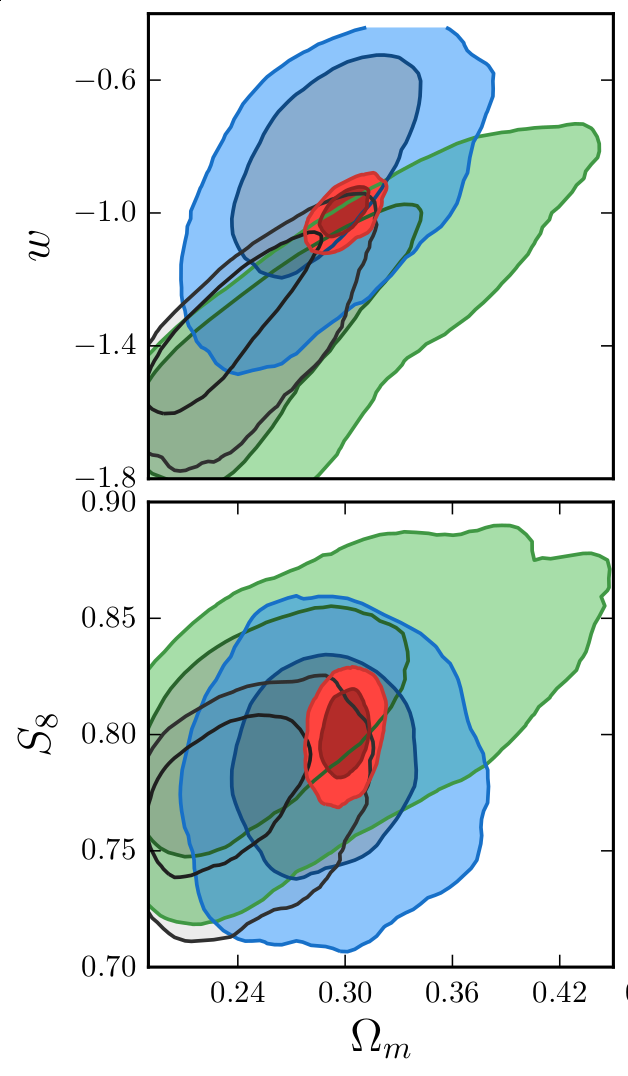
\includegraphics[width=0.8\textwidth]{des-cosmo-w.png}
                \newline
                {\tiny Dark Energy Survey}
            \end{center}
        \end{column}

    \end{columns}


}

\frame
{

    \frametitle{Weak Lensing Shear And Cosmology}

    \setbeamerfont*{itemize/enumerate body}{size=\small}

    \begin{columns}
        \begin{column}{0.5\textwidth}
            \begin{itemize}

                \item At the end of this year we will have results from a lot
                    more lensing data from DES
                    
                \item We will be able to say more about {\color{gold} $w$}
                    independent of other experiments.

            \end{itemize}

        \end{column}
        \begin{column}{0.5\textwidth}
            \begin{center}
                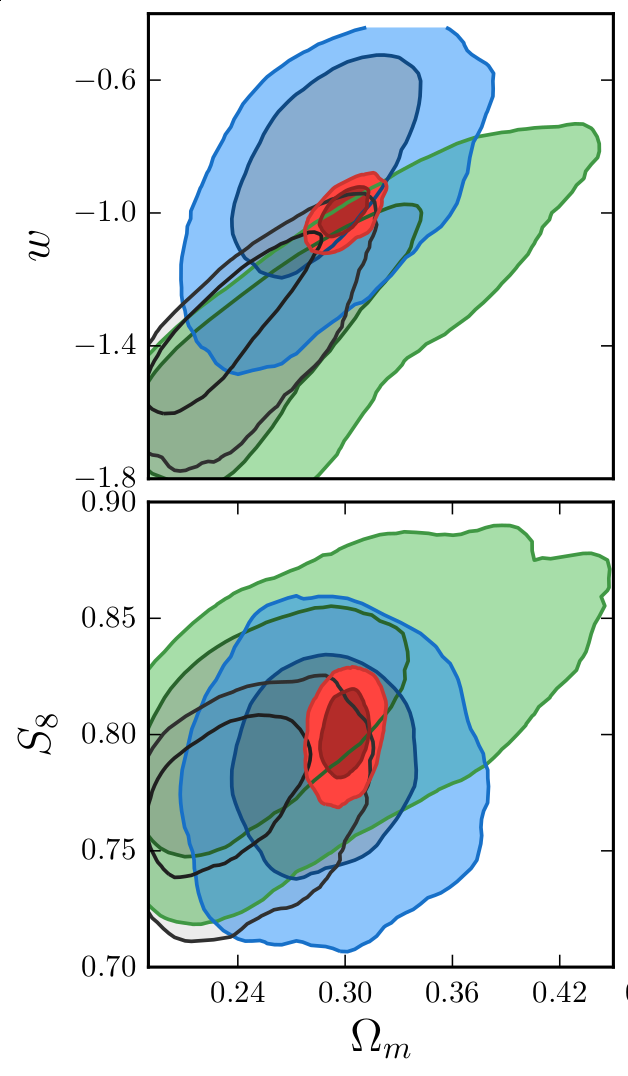
\includegraphics[width=0.8\textwidth]{des-cosmo-w.png}
                \newline
                {\tiny Dark Energy Survey}
            \end{center}
        \end{column}

    \end{columns}


}



\frame
{

    \frametitle{Summary}

    \setbeamerfont*{itemize/enumerate body}{size=\large}

    \begin{columns}
        \begin{column}{0.5\textwidth}
            \begin{itemize}

                \item Lensing is a powerful tool to measure mass in the
                    universe

                \item We can test our theory of the universe and measure the
                    detailed properties of dark matter and dark energy.

                \item Expect exciting results in the near future!

            \end{itemize}

        \end{column}
        \begin{column}{0.5\textwidth}
            \begin{center}
                %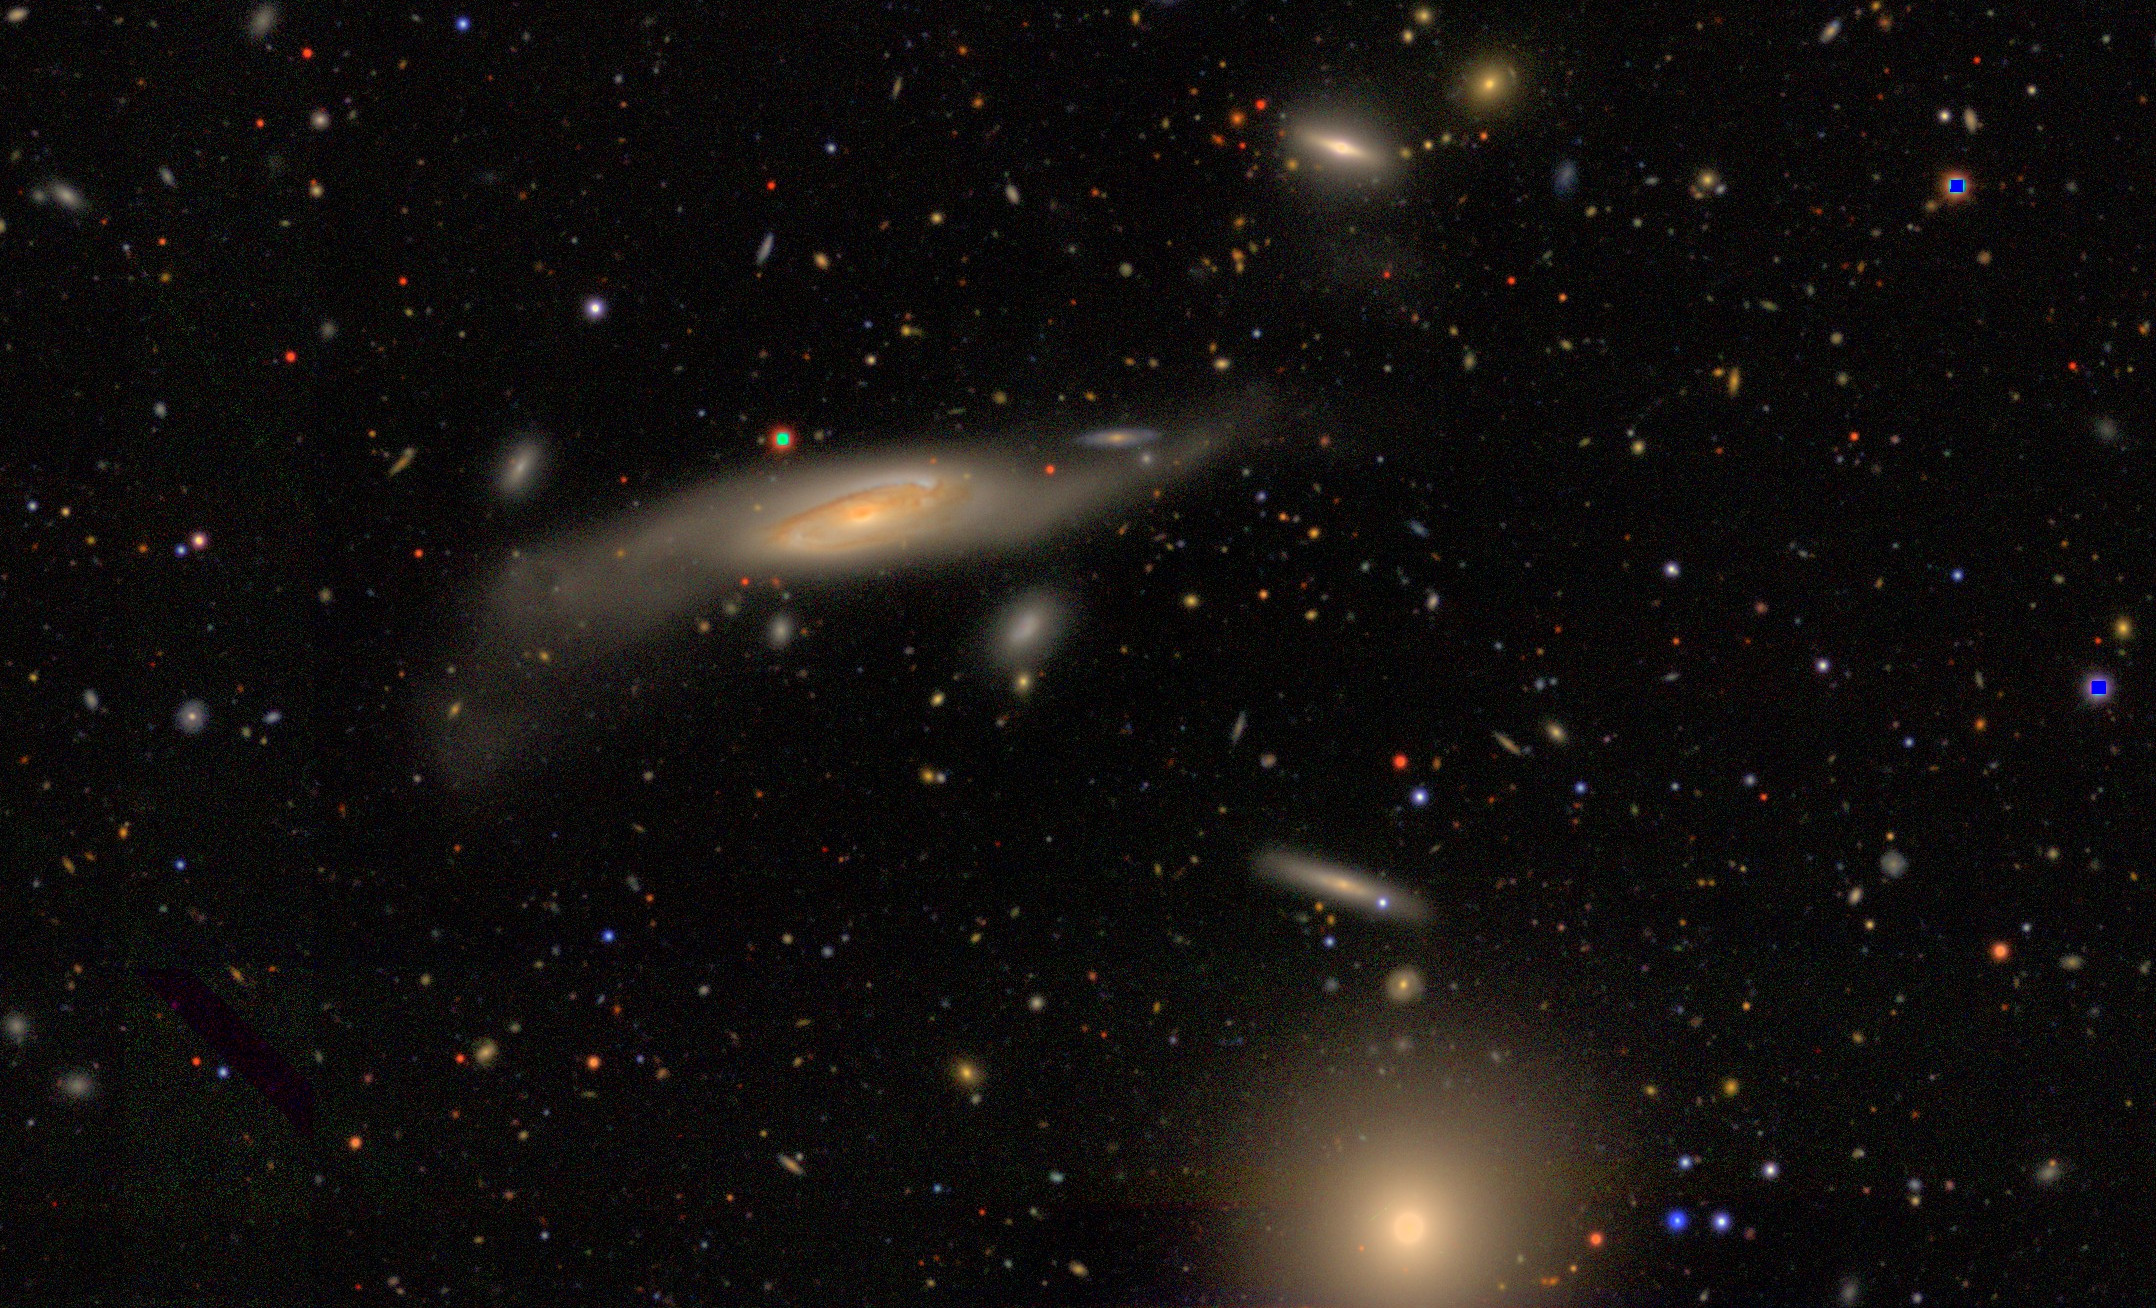
\includegraphics[width=1.2\textwidth, angle=90]{DES0056-5248_gri_crop.jpg}
                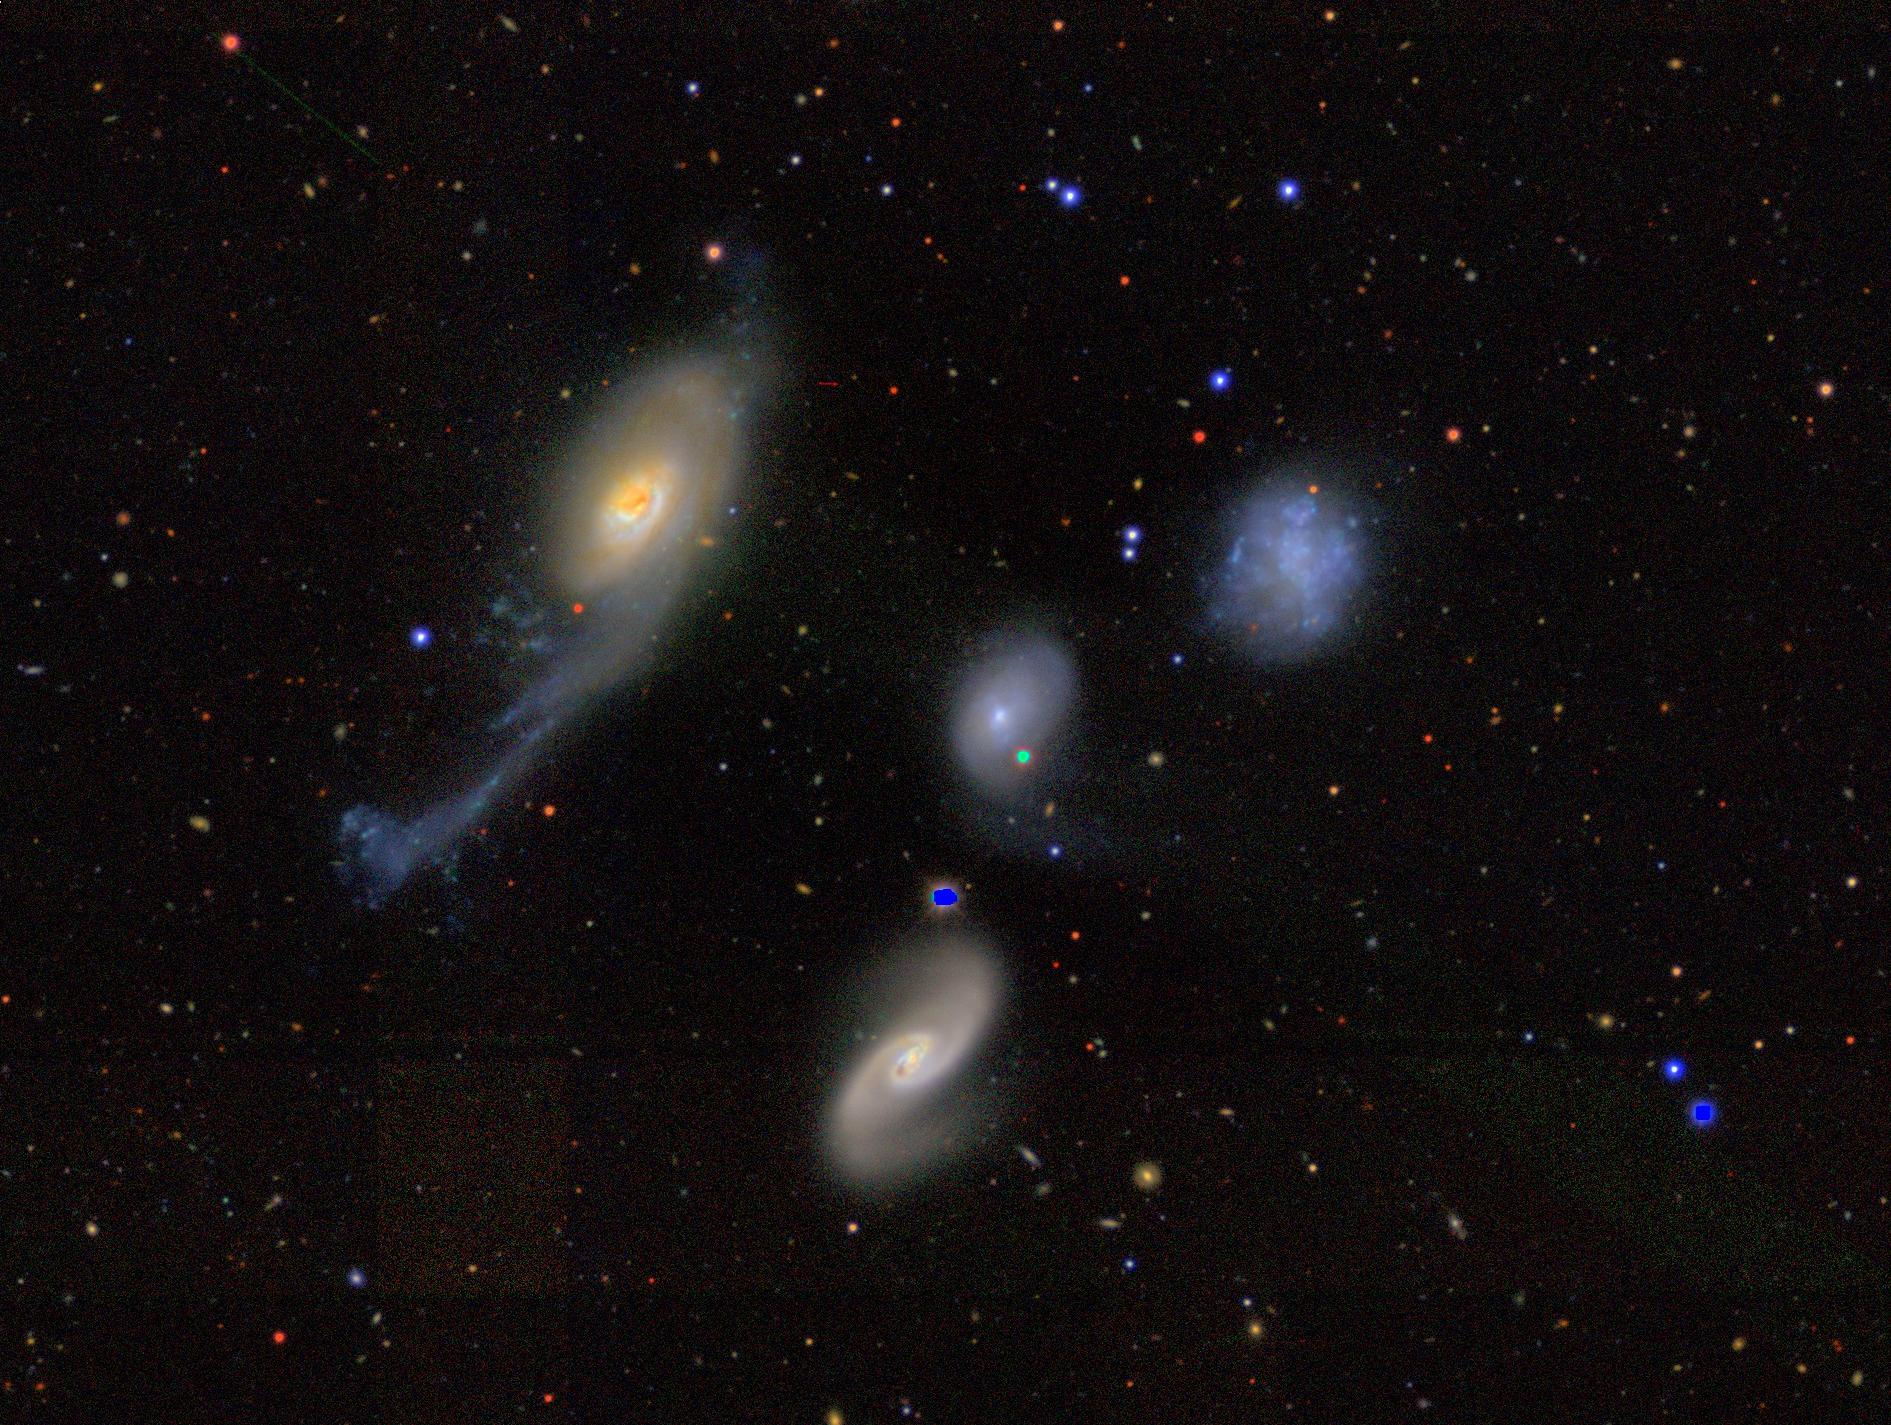
\includegraphics[width=1.2\textwidth, angle=-90]{DES0022-4831-four.jpg}
                \newline
                {\tiny DES/Erin Sheldon}
            \end{center}
        \end{column}

    \end{columns}


}



\end{document}
